\documentclass[11pt]{article}

% Change "review" to "final" to generate the final (sometimes called camera-ready) version.
% Change to "preprint" to generate a non-anonymous version with page numbers.
\usepackage[final]{acl}

% Standard package includes
\usepackage{times}
\usepackage{latexsym}

% For proper rendering and hyphenation of words containing Latin characters (including in bib files)
\usepackage[T1]{fontenc}
% For Vietnamese characters
% \usepackage[T5]{fontenc}
% See https://www.latex-project.org/help/documentation/encguide.pdf for other character sets

% This assumes your files are encoded as UTF8
\usepackage[utf8]{inputenc}

% This is not strictly necessary, and may be commented out,
% but it will improve the layout of the manuscript,
% and will typically save some space.
\usepackage{microtype}

% This is also not strictly necessary, and may be commented out.
% However, it will improve the aesthetics of text in
% the typewriter font.
\usepackage{inconsolata}

%Including images in your LaTeX document requires adding
%additional package(s)
\usepackage{graphicx}
\usepackage{booktabs}
\usepackage{subcaption}
\usepackage{wrapfig}
 \usepackage{multirow} 
% If the title and author information does not fit in the area allocated, uncomment the following
%
%\setlength\titlebox{<dim>}
%
% and set <dim> to something 5cm or larger.

\usepackage{listings}
\usepackage{xcolor}
\usepackage{inconsolata}
\usepackage{makecell}

% 定义代码样式
\definecolor{codegreen}{rgb}{0,0.6,0}
\definecolor{codegray}{rgb}{0.5,0.5,0.5}
\definecolor{codepurple}{rgb}{24, 24, 245}
\definecolor{backcolour}{rgb}{255, 255, 255}

\definecolor{taskblue}{RGB}{0,99,177}
\definecolor{refgreen}{RGB}{0,150,85}
\definecolor{reforange}{RGB}{241, 157, 56}
\definecolor{refpurple}{RGB}{159, 77, 182}
\definecolor{refblue}{RGB}{77, 161, 255}

\definecolor{subviolet}{RGB}{131,76,190}
\definecolor{templateblue}{RGB}{1, 128, 134}
\definecolor{refgreenDark}{RGB}{0, 90, 45}
\definecolor{analysisblue}{HTML}{1E90FF} % Dodger Blue for Analysis boxes
\definecolor{algoyellow}{HTML}{A0522D}   % Brown for Algorithm Description 

\lstdefinestyle{mystyle}{
    backgroundcolor=\color{backcolour},   
    commentstyle=\color{codegreen},
    keywordstyle=\color{magenta},
    numberstyle=\scriptsize\color{codegray},
    stringstyle=\color{codepurple},
    basicstyle=\ttfamily\scriptsize,
    breakatwhitespace=false,         
    breaklines=true,                 
    captionpos=b,                    
    keepspaces=true,                 
    numbers=left,                    
    numbersep=5pt,                  
    showspaces=false,                
    showstringspaces=false,
    showtabs=false,                  
    tabsize=2,
    frame=single,
    rulecolor=\color{black},
    numbers=none  % ← 关闭行号显示
}

% Python listing style
\lstdefinestyle{codestyle}{
  language=Python,
  basicstyle=\footnotesize\ttfamily,
  frame=single,
  numbers=left,
  numberstyle=\scriptsize,
  xleftmargin=1.5em,
  framexleftmargin=1.5em,
  keywordstyle=\color{taskblue},
  commentstyle=\itshape\color{gray},
  stringstyle=\color{orange},
  showstringspaces=false,
  breaklines=true,
  tabsize=2
}

\lstset{
style=mystyle,
  language=C++,
  showstringspaces=false,
  escapeinside={(*@}{@*)},
  literate={\"}{{{}"}}1,
  numbers=none  % ← 关闭行号显示
}



\definecolor{vscode-bg}{RGB}{248,248,248}
\definecolor{vscode-border}{RGB}{220,220,220}
\definecolor{vscode-keyword}{RGB}{0,122,204}
\definecolor{vscode-inline}{RGB}{230,150,50}
\definecolor{vscode-list}{RGB}{150,150,150}
\definecolor{vscode-quote}{RGB}{120,120,120}
\definecolor{vscode-text}{RGB}{40,40,40}

\lstdefinelanguage{Markdown}{
  morecomment=[l][\bfseries\color{vscode-keyword}]{\#},  % 以 # 开头的行
}

\lstdefinestyle{mdstyle}{
  language=Markdown,
  basicstyle=\ttfamily\scriptsize\color{vscode-text},
  backgroundcolor=\color{vscode-bg},
  frame=single,
  rulecolor=\color{vscode-border},
  showstringspaces=false,
  breaklines=true,
  columns=fullflexible,
  breakindent=0pt,        % 关键：换行缩进为0
  % breakatwhitespace=false, % 关键：不在空格处断行
  % postbreak=\mbox{\textcolor{red}{$\hookrightarrow$}\space}, % 可选：显示换行箭头
  aboveskip=6pt,
  belowskip=6pt,
  xleftmargin=0pt,
  xrightmargin=0pt,
  framexleftmargin=0pt,
  framexrightmargin=0pt,
  literate=
    {>}{{\textcolor{vscode-quote}{>}}}1
    {-}{{\textcolor{vscode-list}{-}}}1
    {`}{{\textcolor{vscode-inline}{`}}}1
}



\usepackage{array}          % For advanced table formatting
\usepackage{tabularx}       % For flexible column widths
%%%\usepackage{colortbl}       % For colored table cells and rows
%%%%\usepackage{xcolor}         % For color definitions and text coloring
\usepackage{verbatim}       % For verbatim text blocks
\usepackage{fancyvrb}       % Enhanced verbatim (optional, for better code formatting)
\usepackage{listings}       % Alternative for code formatting (optional)
\usepackage{enumitem}       % For customizing itemize/enumerate lists
\usepackage{amsmath}        % For mathematical formulas
\usepackage{geometry}       % For page layout adjustments (optional)

% Optional packages for better appearance
\usepackage{booktabs}       % For professional table rules
\usepackage{float}          % For better table positioning
\usepackage{caption}        % For better caption formatting

\usepackage{soul}
\usepackage{xcolor}
\usepackage{colortbl}    % 表格行/列着色（\rowcolor）

\usepackage[ruled,vlined,linesnumbered]{algorithm2e}
\usepackage[most]{tcolorbox}
\usepackage{comment}
\definecolor{bggreen}{RGB}{237, 237, 237}
\lstdefinelanguage{json}{
    basicstyle=\ttfamily\small,
    numbers=left,
    numberstyle=\tiny\color{gray},
    stepnumber=1,
    numbersep=8pt,
    showstringspaces=false,
    breaklines=true,
    frame=lines,
    backgroundcolor=\color{gray!5},
    stringstyle=\color{red},
    keywordstyle=\color{blue},
    commentstyle=\color{green!50!black}\itshape,
    morekeywords={true, false, null}
}
%\title{AscendKernelGen: LLM-Driven Kernel Generation for NPUs}

\title{
\Large\textbf{AscendKernelGen: A Systematic Study of LLM-Based Kernel Generation for Neural Processing Units}\\[0.6ex]
\small\textit{System Design, Data Construction, Fine-Tuning, and Comprehensive Evaluation}
}

% Author information can be set in various styles:
% For several authors from the same institution:
% \author{Author 1 \and ... \and Author n \\
%         Address line \\ ... \\ Address line}
% if the names do not fit well on one line use
%         Author 1 \\ {\bf Author 2} \\ ... \\ {\bf Author n} \\
% For authors from different institutions:
% \author{Author 1 \\ Address line \\  ... \\ Address line
%         \And  ... \And
%         Author n \\ Address line \\ ... \\ Address line}
% To start a separate ``row'' of authors use \AND, as in
% \author{Author 1 \\ Address line \\  ... \\ Address line
%         \AND
%         Author 2 \\ Address line \\ ... \\ Address line \And
%         Author 3 \\ Address line \\ ... \\ Address line}

% \author{First Author \\
%   Affiliation / Address line 1 \\
%   Affiliation / Address line 2 \\
%   Affiliation / Address line 3 \\
%   \texttt{email@domain} \\\And
%   Second Author \\
%   Affiliation / Address line 1 \\
%   Affiliation / Address line 2 \\
%   Affiliation / Address line 3 \\
%   \texttt{email@domain} \\}

% \author{
%  \textbf{First Author\textsuperscript{1}},
%  \textbf{Second Author\textsuperscript{1,2}},
%  \textbf{Third T. Author\textsuperscript{1}},
%  \textbf{Fourth Author\textsuperscript{1}},
% \\
%  \textbf{Fifth Author\textsuperscript{1,2}},
%  \textbf{Sixth Author\textsuperscript{1}},
%  \textbf{Seventh Author\textsuperscript{1}},
%  \textbf{Eighth Author \textsuperscript{1,2,3,4}},
% \\
%  \textbf{Ninth Author\textsuperscript{1}},
%  \textbf{Tenth Author\textsuperscript{1}},
%  \textbf{Eleventh E. Author\textsuperscript{1,2,3,4,5}},
%  \textbf{Twelfth Author\textsuperscript{1}},
% \\
%  \textbf{Thirteenth Author\textsuperscript{3}},
%  \textbf{Fourteenth F. Author\textsuperscript{2,4}},
%  \textbf{Fifteenth Author\textsuperscript{1}},
%  \textbf{Sixteenth Author\textsuperscript{1}},
% \\
%  \textbf{Seventeenth S. Author\textsuperscript{4,5}},
%  \textbf{Eighteenth Author\textsuperscript{3,4}},
%  \textbf{Nineteenth N. Author\textsuperscript{2,5}},
%  \textbf{Twentieth Author\textsuperscript{1}}
% \\
% \\
%  \textsuperscript{1}Affiliation 1,
%  \textsuperscript{2}Affiliation 2,
%  \textsuperscript{3}Affiliation 3,
%  \textsuperscript{4}Affiliation 4,
%  \textsuperscript{5}Affiliation 5
% \\
%  \small{
%    \textbf{Correspondence:} \href{mailto:email@domain}{email@domain}
%  }
% }

\author{
 \textbf{Xinzi Cao\textsuperscript{1,3}\thanks{Co-first author}},
 \textbf{Jianyang Zhai\textsuperscript{1,3}\footnotemark[1]},
 \textbf{Pengfei Li\textsuperscript{2}\footnotemark[1]},
 \textbf{Zhiheng Hu\textsuperscript{2}\footnotemark[1]},
 \textbf{Cen Yan\textsuperscript{2}},
 \\
 \textbf{Bingxu Mu\textsuperscript{2}},
 \textbf{Guanghuan Fang\textsuperscript{2}},
 \textbf{Bin She\textsuperscript{2}},
 \textbf{Jiayu Li\textsuperscript{2}},
 \textbf{Yihan Su\textsuperscript{2}}, 
 \textbf{Dongyang Tao\textsuperscript{2}},
 \\
 \textbf{Xiansong Huang\textsuperscript{1}},
 \textbf{Fan Xu\textsuperscript{1}},
 \textbf{Feidiao Yang\textsuperscript{1}},
 \textbf{Yao Lu\textsuperscript{1}},
 \textbf{Chang-Dong Wang\textsuperscript{3}},
 \textbf{Yutong Lu\textsuperscript{3}},
\\
 \textbf{Weicheng Xue\textsuperscript{1}\thanks{Corresponding author}},
 \textbf{Bin Zhou\textsuperscript{1}\footnotemark[2]},
 \textbf{Yonghong Tian\textsuperscript{1,4}\footnotemark[2]}
\\
\\
 \textsuperscript{1}Pengcheng Laboratory,
 \textsuperscript{2}Huawei,
 \textsuperscript{3}Sun Yat-sen University,
 \textsuperscript{4}Peking University
\\
 \small{
   \textbf{Correspondence:} \href{mailto:xuewch@pcl.ac.cn}{xuewch@pcl.ac.cn}, 
   \href{mailto:senosy@gmail.com}{senosy@gmail.com},
   \href{mailto:yhtian@pku.edu.cn}{yhtian@pku.edu.cn}
 }
}
\begin{document}
\maketitle
\begin{abstract}
To meet the ever-increasing demand for computational efficiency, Neural Processing Units (NPUs) have become critical in modern AI infrastructure. However, unlocking their full potential requires developing high-performance compute kernels using vendor-specific Domain-Specific Languages (DSLs), a task that demands deep hardware expertise and is labor-intensive. While Large Language Models (LLMs) have shown promise in general code generation, they struggle with the strict constraints and scarcity of training data in the NPU domain. Our preliminary study reveals that state-of-the-art general-purpose LLMs fail to generate functional complex kernels for Ascend NPUs, yielding a near-zero success rate. To address these challenges, we propose AscendKernelGen, a generation-evaluation integrated framework for NPU kernel development. We introduce Ascend-CoT, a high-quality dataset incorporating chain-of-thought reasoning derived from real-world kernel implementations, and KernelGen-LM, a domain-adaptive model trained via supervised fine-tuning and reinforcement learning with execution feedback. Furthermore, we design NPUKernelBench, a comprehensive benchmark for assessing compilation, correctness, and performance across varying complexity levels. Experimental results demonstrate that our approach significantly bridges the gap between general LLMs and hardware-specific coding. Specifically, the compilation success rate on complex Level-2 kernels improves from 0\% to 95.5\% (Pass@10), while functional correctness achieves 64.3\% compared to the baseline's complete failure. These results highlight the critical role of domain-specific reasoning and rigorous evaluation in automating accelerator-aware code generation. AscendKernGen is available at \href{https://huggingface.co/AscendKernelGen}{\textcolor{blue}{AscendKernGen}} and \href{https://github.com/weich97/NPUKernelBench}{\textcolor{blue}{NPUKernelBench}}.
\end{abstract}

\section{Introduction}

The rapid advancement of Artificial Intelligence (AI), particularly deep learning, has fundamentally reshaped modern computing architectures. To meet the ever-increasing demand for computational efficiency and throughput, domain-specific accelerators have emerged as a key solution. Among them, Neural Processing Units (NPUs), such as Huawei's Ascend platform~\cite{liao2021ascend, xue2024unlocking, wroblewski2025parallel}, play a critical role in contemporary AI infrastructure by providing high performance for deep learning workloads. However, the practical efficiency of these accelerators is determined not only by hardware capabilities, but also by the quality of the underlying compute kernels. As a result, developing high-performance, hardware-adapted kernels is a prerequisite for fully unlocking the potential of NPU platforms.

Writing such kernels remains extremely challenging. NPU kernel development typically relies on highly specialized, vendor-specific domain-specific languages (DSLs), such as AscendC, which require developers to possess deep expertise in hardware architecture. This includes fine-grained management of hierarchical memory systems (e.g., global versus on-chip memory), carefully designed data tiling strategies, asynchronous pipeline programming for overlapping computation and data movement, and explicit utilization of vector (SIMD) and matrix (Cube) execution units. The resulting learning curve is steep, making manual kernel development time-consuming, costly, and error-prone. Consequently, kernel optimization has become a major bottleneck in the rapid iteration and deployment of AI applications on NPU architectures.

At a higher level, this challenge exposes a fundamental limitation of current code generation approaches: general-purpose programming knowledge is insufficient for generating correct and efficient code in highly specialized, hardware-specific domains. Motivated by the success of Large Language Models (LLMs) in general-purpose code generation, both academia and industry have explored their use for automating kernel development. However, this approach faces a critical obstacle. The knowledge required for hardware-specific DSLs differs fundamentally from that of general-purpose programming languages, encompassing strict API constraints, architecture-dependent semantics, and performance-critical optimization patterns. Moreover, high-quality training data in this domain is extremely scarce, leaving general-purpose LLMs poorly equipped to handle such tasks.

Our preliminary evaluation, summarized in Table~\ref{tab:zero_shot_perf}, confirms this limitation empirically. Even state-of-the-art general-purpose LLMs (e.g., Qwen 3) perform extremely poorly when generating AscendC kernels in a zero-shot setting. These models frequently hallucinate non-existent APIs (e.g., \texttt{AscendC::Softmax}) or severely misuse core hardware interfaces, leading to exceptionally high compilation failure rates. For complex L2/L3 kernels, the execution success rate drops to around 0\%, indicating that, without domain-specific adaptation, general-purpose LLMs are effectively unusable for non-trivial NPU kernel development.

\begin{table}[htbp]
  \centering
  \caption{Zero-shot performance of general-purpose LLMs on the NPUKernelBench benchmark.}
  \label{tab:zero_shot_perf}
  \begin{tabular}{llcc}
    \toprule
    \textbf{Model} & \textbf{Task Type} & \textbf{Compilation} & \textbf{Functional Correctness} \\
     & & \textbf{Success Rate} & \textbf{(Post-Compilation)} \\
    \midrule
    \multirow{2}{*}{Qwen3-8B} & L1 (Simple) & 8.22\% & 1.08\% \\
     & L2/L3 (Complex) & 1.39\% & 0.00\% \\ \hline
     %\multirow{2}{*}{Qwen2.5-7B} & L1 (Simple) & 16.58\% & 1.89\% \\
     %& L2/L3 (Complex) & 6.89\% & 0.11\% \\ \hline
     \multirow{2}{*}{Qwen2.5-Coder-7B} & L1 (Simple) & 9.19\% & 0.47\% \\
     & L2/L3 (Complex) & 0.40\% & 0.00\% \\ \hline
     \multirow{2}{*}{Llama3.1-8B} & L1 (Simple) & 23.97\% & 0.69\% \\
     & L2/L3 (Complex) & 19.44\% & 0.00\% \\ \hline
     \multirow{2}{*}{Mistral-7B} & L1 (Simple) & 0.00\% & 0.00\% \\
     & L2/L3 (Complex) & 0.00\% & 0.00\% \\
    \bottomrule
  \end{tabular}
\end{table}

These observations suggest that enabling LLMs to generate high-quality NPU kernels requires two key advancements. First, the model must acquire a deep understanding of the hardware-specific programming paradigm, including API constraints and architectural characteristics. Second, a professional and reliable evaluation framework is necessary to rigorously assess not only compilation success, but also functional correctness and performance, which are all critical for kernel-level code.

To address these challenges, we propose \textbf{AscendKernelGen}, a generation--evaluation integrated framework for NPU kernel development. Our contributions are threefold:

\begin{enumerate}
    \item \textbf{A Domain-Specific Reasoning Dataset for Kernel Generation.}
    We construct and release \textit{Ascend-CoT}, a high-quality dataset designed to capture the structured reasoning processes required for low-level NPU kernel programming. The dataset is curated from real-world kernel implementations and includes detailed annotations that reflect pipeline construction, synchronization logic, and arithmetic reasoning patterns.

    \item \textbf{Domain-Adaptive Post-Training for Low-Level Code Generation.}
    Building on a strong base LLM, we introduce a domain-adaptive post-training strategy that explicitly targets the reasoning challenges of NPU kernel synthesis. The resulting model, \textit{KernelGen-LM}, demonstrates substantially improved compilation success and functional correctness compared to general-purpose code models.

    \item \textbf{A Comprehensive Evaluation Benchmark for NPU Kernels.}
    We design \textit{NPUKernelBench}, an evaluation framework that systematically assesses generated kernels along three dimensions: compilation success, functional correctness, and performance. Its dual-path evaluation design enables rigorous analysis of both static-shape optimization and dynamic-shape robustness, providing a reliable benchmark for future research on accelerator-aware code generation.
\end{enumerate}

Experimental results demonstrate the effectiveness of the proposed approach.
After domain-adaptive post-training on the \texttt{Ascend-CoT} dataset, the model exhibits substantial improvements in kernel generation quality, particularly on complex kernels that are nearly unsolvable in zero-shot settings.
Both compilation success and functional correctness improve consistently across difficulty levels, indicating that domain-specific reasoning supervision is crucial for bridging the gap between general-purpose LLMs and hardware-specific kernel programming.

The remainder of this work is organized as follows.
Section~\ref{sec:relatedworks} reviews prior research on LLM-based code generation, traditional hardware-specific kernel optimization and benchmarks for code generation.
Section~\ref{sec:programming_constraints} introduces the programming abstractions and hardware constraints that characterize NPU kernel development.
Section~\ref{sec:system_overview} presents an overview of the \texttt{AscendKernelGen} framework, covering both the kernel generation pipeline and the hardware-grounded evaluation workflow.
Section~\ref{data_construct} describes the construction of the training data, including documentation-based CoT, code-centric CoT, and general CoT data.
Section~\ref{fine_tune} details the domain-adaptive fine-tuning process for LLM-based NPU kernel generation.
Section~\ref{NPUKernelBench} introduces \texttt{NPUKernelBench}, our evaluation benchmark for assessing compilation, correctness, and performance on real NPU hardware.
Section~\ref{experiments} reports the experimental setup and provides an in-depth analysis of the empirical results.
Finally, Section~\ref{conclusions} concludes the report and discusses directions for future work.
\section{Related Works}
\label{sec:relatedworks}

Our work lies at the intersection of large-scale model–based code generation and hardware-specific kernel optimization. In this section, we review prior work from four perspectives: general-purpose code generation with LLMs, traditional hardware kernel optimization, LLM-based kernel generation, and benchmarking for code generation.

\subsection{Large-Scale Models for General-Purpose Code Generation}

Large Language Models (LLMs) have demonstrated remarkable progress in general-purpose code generation across mainstream programming languages such as Python, C++, and Java. Representative systems include OpenAI's Codex~\cite{chen2021evaluating}, AlphaCode~\cite{novikov2025alphaevolve}, Code Llama~\cite{roziere2023code}, Qwen2.5/3-Coder~\cite{hui2024qwen2}, and CodeRL~\cite{le2022coderl}, enabling applications such as code completion, refactoring, and competitive programming.

Despite these advances, general-purpose LLMs remain limited when applied to domain-specific code generation tasks that involve specialized APIs and strict semantic constraints~\cite{gu2025effectiveness}. In particular, hardware-specific programming languages impose requirements that differ fundamentally from general-purpose software development, including explicit memory hierarchy management, architecture-dependent execution semantics, and performance-critical correctness constraints. When faced with such settings, LLMs often fail to generate compilable or semantically valid code, motivating the need for domain-adaptive data and training strategies.


\subsection{Traditional Hardware-Specific Kernel Optimization}

%Before the advent of LLMs, academia and industry primarily relied on traditional AI compilers and auto-tuning techniques to optimize kernels on specific hardware. These routes include:

%\begin{itemize}
%    \item Auto-Tuning: Techniques like TVM~\cite{chen2018tvm} and Ansor~\cite{zheng2020ansor} optimize performance through operator splitting, fusion, and scheduling combined with automated search.
%    \item High-Level Abstractions \& Domain-Specific Languages: Halide~\cite{ragan2013halide} pioneered the decoupling of algorithm definition from execution scheduling, significantly simplifying the optimization of image processing pipelines across diverse architectures. Similarly, Triton~\cite{tillet2019triton} simplify GPU kernel development via a high-level, Python-like abstraction, while MLIR~\cite{lattner2020mlir} provides modular intermediate representation capabilities. TensorFlow XLA follows a similar compiler-based route, lowering high-level TensorFlow graphs into high-level optimizer intermediate representation and performing aggressive fusion and optimization before generating backend-specific code for platforms with different architecture~\cite{snider2023operator}. PyTorch 2.0 further extends this route through TorchDynamo and TorchInductor~\cite{ansel2024pytorch}, where the former captures Python-level computation graphs with minimal overhead and the latter compiles them into optimized GPU (Triton) or CPU (C++) kernels, achieving substantial real-world speedups across large model suites.
%    \item \textbf{Polyhedral Compilation:} Approaches like Tensor Comprehensions~\cite{vasilache2018tensor} and Tiramisu~\cite{baghdadi2019tiramisu} utilize polyhedral intermediate representations to perform systematic loop transformations. AKG~\cite{zhao2021akg} specifically targets Neural Processing Units (NPUs) like Huawei Ascend. It leverages polyhedral schedulers to model the NPU's heterogeneous compute units (Cube/Vector) and automate the management of its complex memory hierarchy via integer linear programming.
%    \item Search \& Equivalent Transformation: Frameworks like TASO~\cite{jia2019taso}, PET~\cite{wang2021pet}, and EINNET~\cite{zheng2023einnet} automatically explore efficient execution plans by formalizing operator specifications or transforming tensor algebra expressions.
%    \item Platform-Specific Libraries: NVIDIA's CUTLASS~\cite{markidis2018nvidia}, for instance, provides a template library for tensor operations to generate optimized CUDA kernels. Similarly, Liger-Kernel~\cite{hsu2024liger} offers a set of Triton-based kernels that are explicitly optimized for both a specific hardware platform (GPUs) and a specific workload (LLM training), enabling substantial improvements in training throughput and memory efficiency over baseline implementations.
%\end{itemize}


%While these methods can achieve high performance, they are often constrained by a dependency on extensive expert knowledge (e.g., for template design), prohibitive search times (for Auto-Tuning), and limited generalization capabilities. These distinct approaches, spanning TVM's general-purpose tuning, the specialized abstractions of Triton/TASO/PET/EINNET, and dedicated libraries like CUTLASS, all fail to directly adapt to closed-structure, interface-specific architectures such as the Ascend NPU. This highlights a critical dilemma: general-purpose solutions (like TVM) lack the necessary adaptability for this target, while platform-specific solutions (like CUTLASS) incur high development costs and offer no performance portability. This motivates our LLM-based generation approach.

Prior to the adoption of LLMs, kernel optimization for specialized hardware primarily relied on compiler-based and auto-tuning approaches. Auto-tuning frameworks such as TVM~\cite{chen2018tvm} and Ansor~\cite{zheng2020ansor} search over scheduling and optimization spaces to improve performance across diverse hardware backends. High-level abstractions and domain-specific languages, including Halide~\cite{ragan2013halide}, Triton~\cite{tillet2019triton}, and MLIR~\cite{lattner2020mlir}, decouple algorithm specification from execution scheduling, substantially lowering the barrier to kernel optimization on GPUs and other accelerators. Similarly, TensorFlow XLA~\cite{snider2023operator} and PyTorch 2.0~\cite{ansel2024pytorch} adopt compiler-based pipelines to transform high-level computation graphs into optimized backend-specific kernels.

More specialized approaches leverage polyhedral compilation techniques to model and optimize loop transformations systematically. Representative systems include Tensor Comprehensions~\cite{vasilache2018tensor}, Tiramisu~\cite{baghdadi2019tiramisu}, and AKG~\cite{zhao2021akg}, the latter of which targets NPUs by modeling heterogeneous compute units and complex memory hierarchies. Other efforts explore operator-level search and algebraic transformation, such as TASO~\cite{jia2019taso}, PET~\cite{wang2021pet}, and EINNET~\cite{zheng2023einnet}. In addition, platform-specific libraries like CUTLASS~\cite{markidis2018nvidia} and Liger-Kernel~\cite{hsu2024liger} provide hand-optimized kernels for particular hardware–workload combinations.

While these methods can achieve high performance, they typically require substantial expert knowledge, incur high search or development costs, and offer limited generalization across architectures. General-purpose compilers often lack the flexibility to adapt to closed or interface-constrained platforms, whereas platform-specific libraries sacrifice portability. These limitations motivate exploration of more flexible, learning-based kernel generation approaches.


\subsection{LLM-based Generation for Hardware Kernels}

\begin{comment}

Recently, a series of pioneering works have begun exploring the use of LLMs to generate hardware code (rather than Python), showing significant potential. These efforts are primarily concentrated in the mature CUDA and TPU ecosystems:

\begin{itemize}
    \item \textbf{GPU Kernels:} Research in the GPU ecosystem exhibits a diverse methodological spectrum.
    \begin{itemize}
        \item \textbf{Direct generation via in-context learning (prompting):}
        Ouyang et al.~\cite{ouyang2025kernelbench} proposed KernelBench to evaluate the ability of LLMs to generate CUDA kernels. CUDA-LLM~\cite{chen2025cuda} utilizes LLMs to automatically generate and optimize CUDA programs. Sakana.ai's AI CUDA Engineer~\cite{lange2025ai} proposes using intermediate representations to improve LLM understanding of low-level operators. 
    
        \item \textbf{Domain adaptation via supervised fine-tuning (SFT):}
        Fisches et al.~\cite{kernelllm2025} proposed KernelLLM, a model trained specifically for generating Triton GPU kernels that achieves competitive performance despite its relatively small size.

        \item \textbf{Optimization via reinforcement learning (RL):}
        Baronio et al. proposed Kevin~\cite{baronio2025kevin}, the first model trained with a multi-turn GRPO~\cite{shao2024deepseekmath, guo2025deepseek} for CUDA kernel generation and optimization, which significantly improves correctness and performance by explicitly incorporating iterative refinement and leveraging execution feedback across turns. Li et al. introduced CUDA-L1~\cite{li2025cuda}, a pipelined system for CUDA optimization powered by a novel Contrastive Reinforcement Learning (Contrastive-RL) algorithm, achieving an industry-leading average speedup of $3.12\text{x}$ (median $1.42\text{x}$) over default baselines on KernelBench by autonomously discovering and strategically combining optimization techniques across different GPU architectures. Li et al. introduced AutoTriton~\cite{li2025autotriton}, the first RL-powered model for Triton programming, which sequentially leverages a specialized data pipeline for supervised fine-tuning and applies the GRPO algorithm with a combined rule-based and execution-based reward to achieve correctness and performance comparable to mainstream large LLMs. Woo et al. introduced TritonRL~\cite{woo2025tritonrl}, an 8B-scale Triton-specific LLM trained with a novel RL framework featuring a robust, fine-grained verifier (mitigating reward hacking) and a hierarchical reward decomposition for reasoning and code tokens, achieving state-of-the-art correctness and speedup among small Triton models. SparseRL~\cite{anonymous2025mastering} is a Deep Reinforcement Learning framework for sparse CUDA code generation (SpMV/SpMM) that utilizes a novel sinusoidal embedding of sparse matrix indices and a hierarchical reward function incorporating execution efficiency, achieving state-of-the-art performance with up to $30\%$ faster code execution compared to existing LLM methods.
    
        \item \textbf{Autonomous generation via agentic frameworks:}
        Guo et al.~\cite{guo2025evoengineer} introduced EvoEngineer, the first systematic framework for LLM-based CUDA kernel code evolution that decomposes the process into two-layer traverse techniques and population management. Dong et al.~\cite{dong2025stark} introduced STARK, a novel multi-agent LLM framework for GPU kernel optimization that employs specialized agents for planning, coding, and debugging, coupled with a strategic search over a tree memory and grounded instructions to consistently achieve substantial runtime speedups (up to 16x) over conventional monolithic agents. Zhang et al. proposed CudaForge~\cite{zhang2025cudaforge}, a novel training-free multi-agent workflow (Coder and Judge) for CUDA kernel optimization that explicitly integrates Nsight Compute (NCU) hardware feedback to guide targeted, iterative refinement, achieving state-of-the-art correctness ($97.6\%$) and high speedup ($1.68\text{x}$) at a remarkably low API cost.

        \item \textbf{Other techniques:}
        Gong et al. proposed ReGraphT~\cite{gong2025large}, a training-free retrieval-augmented generation framework that transfers LLM-level CUDA optimization expertise to small language models by encoding optimization trajectories into a structured Reasoning Graph and leveraging Monte Carlo Graph Search for efficient, guided exploration, achieving significant speedups.
    \end{itemize}
    
    \item \textbf{TPU Kernels:} Google DeepMind's AlphaEvolve~\cite{novikov2025alphaevolve} is a Gemini-based evolutionary coding agent capable of optimizing TPU arithmetic circuits and AI training kernels (like FlashAttention).
    \item \textbf{HPC (High-Performance Computing):} Several US National Labs (ORNL, LLNL, ANL, etc.) are also developing LLM-driven HPC agents for performance analysis and parallel code generation~\cite{teranishi2025leveraging, ma2025connecting, nichols2024hpc, chaturvedi2025hpc}.
\end{itemize}

While these groundbreaking works demonstrate the feasibility of LLM-based hardware code generation, their focus on the mature CUDA and TPU ecosystems highlights two critical gaps that motivate our work. First, they do not address the unique architectural challenges and proprietary programming paradigm of the Ascend NPU platform. Second, they lack a public, systematic evaluation framework specifically designed to benchmark AscendC kernel generation. As a result, applying LLM-based automation frameworks to the emerging Ascend ecosystem remains a largely unexplored niche. This situation clearly demonstrates the necessity for both our generation model and evaluation framework.

\end{comment}

Inspired by the success of LLMs in general-purpose programming, recent work has begun to explore their application to hardware kernel generation, primarily within mature ecosystems such as CUDA GPUs and TPUs. Early efforts focus on direct kernel generation via prompting and in-context learning, as exemplified by CUDA-LLM~\cite{chen2025cuda} and AI CUDA Engineer~\cite{lange2025ai}. Subsequent work introduces domain adaptation through supervised fine-tuning, such as KernelLLM~\cite{kernelllm2025}, which demonstrates that compact, domain-specific models can generate competitive GPU kernels.

More recent studies incorporate reinforcement learning and execution feedback to iteratively refine generated kernels. Systems such as Kevin~\cite{baronio2025kevin}, CUDA-L1~\cite{li2025cuda}, AutoTriton~\cite{li2025autotriton}, and TritonRL~\cite{woo2025tritonrl} show that combining supervised initialization with execution-guided optimization can significantly improve correctness and performance. In parallel, agentic and multi-agent frameworks have been proposed to automate kernel optimization through planning, debugging, and search, including EvoEngineer~\cite{guo2025evoengineer}, STARK~\cite{dong2025stark}, and CudaForge~\cite{zhang2025cudaforge}. Related efforts also explore retrieval-augmented and graph-based reasoning for kernel optimization~\cite{gong2025large}.

Despite these advances, existing LLM-based kernel generation methods largely focus on open and well-documented platforms such as CUDA and TPU, benefiting from mature toolchains and abundant training data. In contrast, LLM-driven kernel generation for emerging NPU platforms with proprietary programming models remains underexplored.


\subsection{Benchmarking for Code Generation}

\begin{comment}

The evaluation of LLM-generated code was standardized in the general-purpose domain by benchmarks such as \texttt{HumanEval}~\cite{chen2021evaluating} and \texttt{MBPP}~\cite{austin2021program}. However, these frameworks are fundamentally unsuitable for the NPU kernel domain. They primarily evaluate functional correctness on algorithmic tasks and do not measure the critical metrics essential to hardware programming, such as \textit{compilation success}, \textit{functional correctness} under hardware constraints, or \textit{performance} (e.g., latency, throughput).

This gap led to the creation of the first hardware-specific benchmarks, most notably \texttt{KernelBench} (for CUDA) and \texttt{MultiKernelBench} (for multiple platforms, including AscendC). While these frameworks represent a significant step forward by introducing compilation and performance metrics, our analysis reveals that they possess a key architectural limitation: they tend to operate as single-path evaluation systems. For instance, existing frameworks typically support only one "Host+Device" evaluation paradigm. This requires the LLM to \textit{always} generate the complete Host-side and Device-side code, even for simple kernels. This "single-path" architecture lacks flexibility, forcing the model to generate a large amount of complex Host-Side boilerplate code for simple tasks (like L1 kernels), which adds unnecessary evaluation difficulty.

In the area of automated GPU kernel development, TritonGym~\cite{anonymous2025tritongym} is an interactive, tool-centric benchmark and orchestration framework that standardizes access to evaluation tools via a function-call API, enabling fair comparison and systematic evaluation of agentic LLM workflows for Triton GPU kernel generation, especially for challenging out-of-distribution (OOD) tasks.

To the best of our knowledge, there remains a critical need for a flexible evaluation framework that can appropriately assess LLMs on both simple "Kernel-Only" tasks and complex, "Host+Device" tasks, thereby providing a more comprehensive evaluation of both static shape optimization and dynamic shape robustness.

\end{comment}

Evaluation of LLM-generated code in general-purpose domains has been standardized by benchmarks such as HumanEval~\cite{chen2021evaluating} and MBPP~\cite{austin2021program}. However, these benchmarks focus primarily on functional correctness and are ill-suited for hardware kernel generation, where compilation success, hardware-constrained correctness, and performance metrics are equally critical.

To address this gap, hardware-oriented benchmarks such as KernelBench~\cite{ouyang2025kernelbench} and MultiKernelBench~\cite{wen2025multikernelbench} extend evaluation to include compilation and performance. While these benchmarks represent an important step forward, they typically adopt a single-path evaluation paradigm that requires generation of complete host–device code for all tasks. This design introduces unnecessary complexity for simple kernels and limits flexibility in assessing different levels of kernel abstraction. More recent systems, such as TritonGym~\cite{anonymous2025tritongym}, provide interactive and tool-centric evaluation environments for GPU kernels.

Overall, there remains a lack of a flexible, comprehensive evaluation framework tailored to NPU kernel generation that can jointly assess kernel-only optimization and full host–-device integration. Addressing this gap is essential for reliably measuring progress in LLM-based kernel generation for specialized hardware platforms.
\section{Programming Abstractions and Constraints for NPU Kernel Generation}
\label{sec:programming_constraints}

\begin{comment}

\subsection{Ascend NPU: DaVinci Architecture}
\label{sec:hardware_arch}

The Ascend 910B1 NPU leverages the advanced DaVinci architecture, characterized by a decoupled heterogeneous computing paradigm that physically segregates matrix and vector processing to maximize computational efficiency. As illustrated in Figure~\ref{fig:NPU}, where arrows denote the directional data processing flow, the architecture is fundamentally divided into two independent execution engines: the Matrix Computation Engine (AI Cube, or AIC) and the Vector Computation Engine (AI Vector, or AIV). To achieve massive parallelism, each NPU integrates 25 AICs and 50 AIVs, culminating in a peak computing performance of 379 TFLOPS in FP16 precision.

The AIC (top section) is specialized for high-throughput tensor operations, employing a hierarchical memory structure managed by dedicated Memory Transfer Engines (MTE1/MTE2/MTE3). Data is prefetched from Global Memory (GM) into an on-chip L1 Buffer and subsequently distributed to Buffer L0A and Buffer L0B to feed the CUBE unit for matrix multiplication, with results accumulated in Buffer L0C. The architecture incorporates specialized on-chip storage to accelerate post-processing: the BT Buffer is designated for storing bias values, while the Fixpipe Buffer holds quantization and ReLU parameters. Conversely, the AIV (bottom section) handles complex element-wise and scalar logic, centered around a massive Unified Buffer (UB) that serves both the Scalar Unit and the Vector Unit. A critical feature of this split-core design is the independence of the instruction streams; the AIC and AIV can load separate code segments and execute asynchronously, coupled only by data exchange through the Global Memory. This decoupling allows for fine-grained software scheduling, enabling the massive parallelism of the Cube units to operate concurrently with the flexible logic of the Vector units, thereby optimizing the overall throughput for diverse deep learning workloads.

\begin{figure}[t]
    \centering
    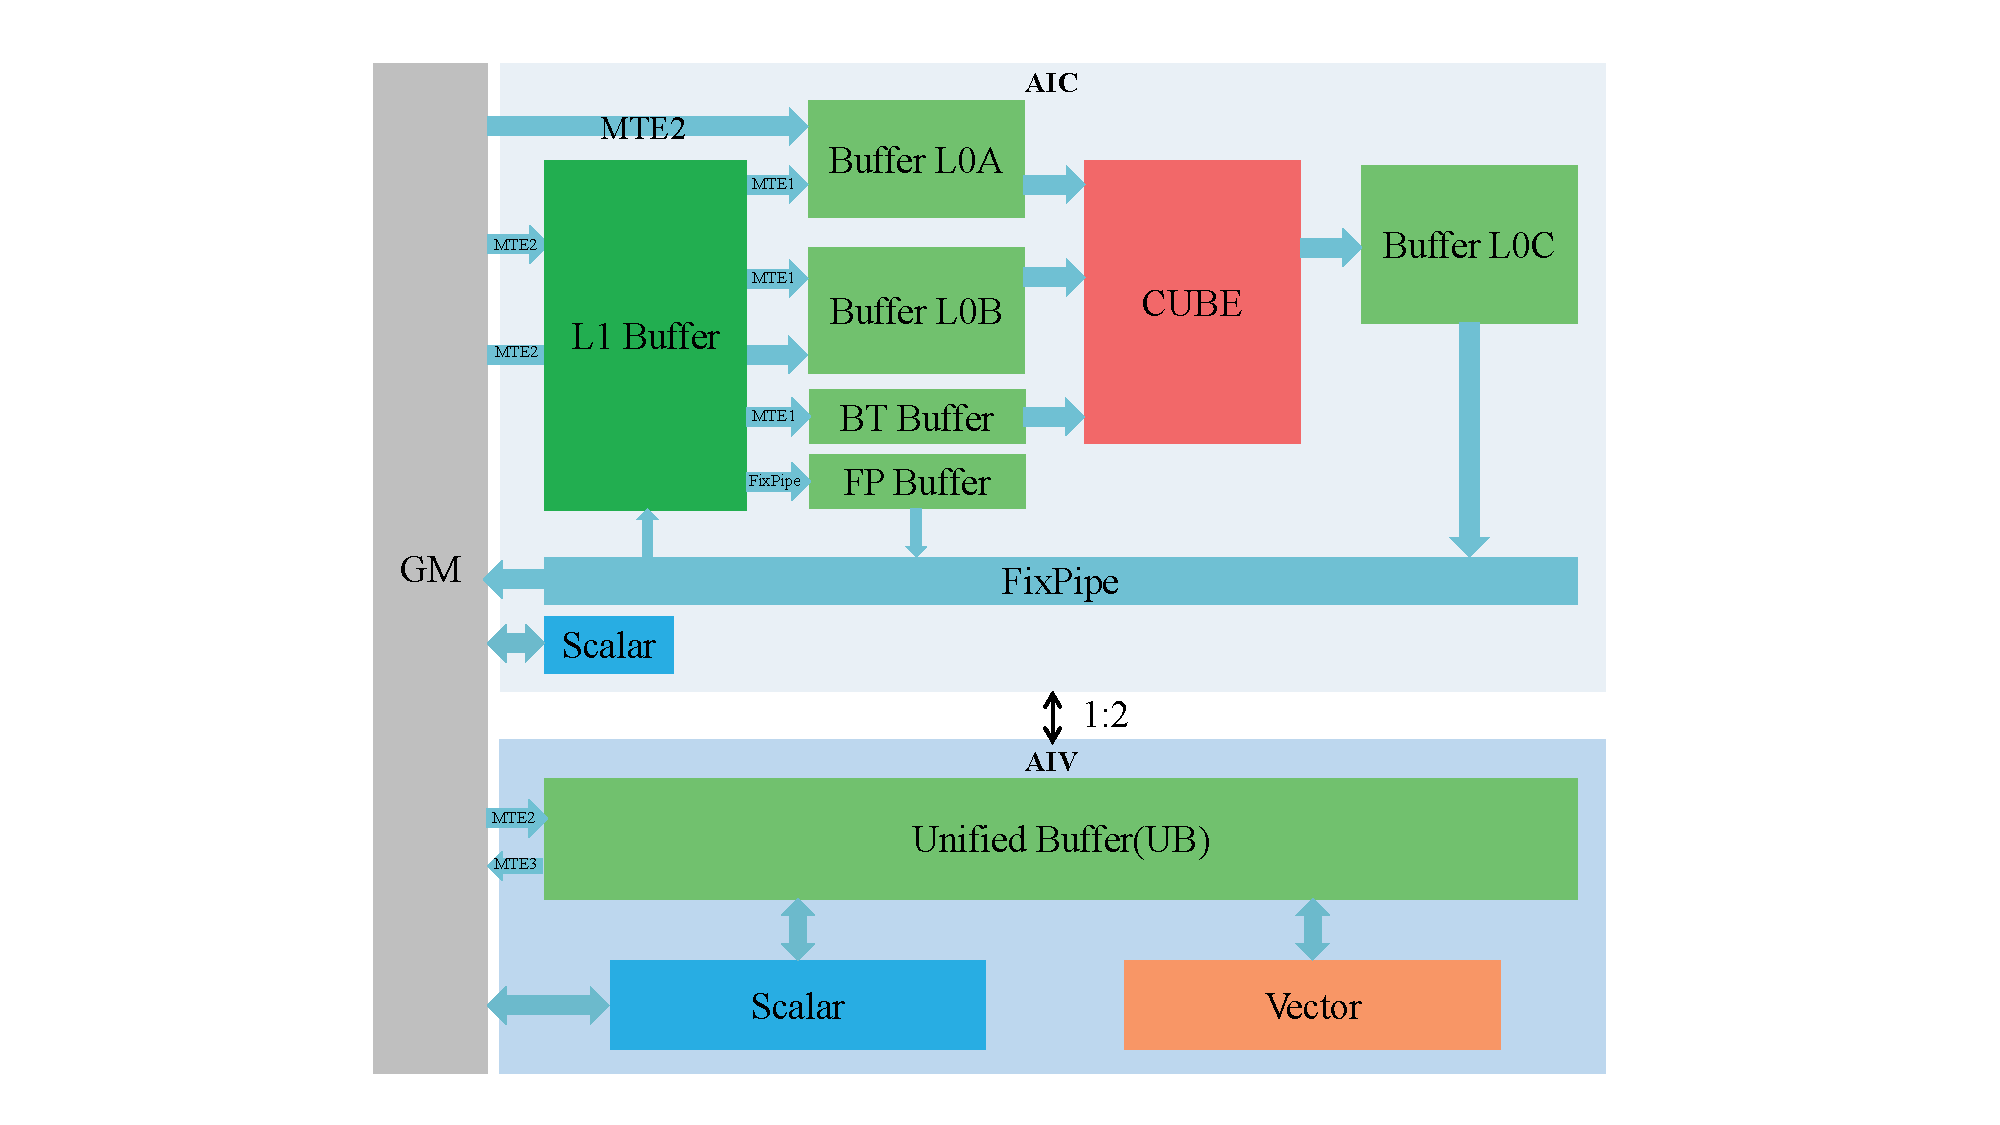
\includegraphics[width=0.6\linewidth, trim={6.4cm 1.0cm 6.6cm 1.0cm}, clip]{pdfs/910B.pdf}
    \caption{DaVinci architecture of Huawei Ascend 910B1 NPU}
    \label{fig:NPU}
\end{figure}

\subsection{Ascend Programming Model: SPMD and Pipeline Parallelism}
\label{sec:programming_model}

To abstract the complexity of the underlying heterogeneous hardware while exposing its massive parallelism, the Ascend processor employs a programming model characterized by Single-Program Multiple-Data (SPMD) execution and Asynchronous Pipeline Parallelism. This model provides the necessary structural template that our generation framework follows.

\paragraph{SPMD Execution Paradigm}
The Ascend NPU adopts the SPMD model to scale computational throughput. A single kernel function is instantiated across multiple AI Cores simultaneously. All cores execute the exact same instruction stream, but operate on disjoint data partitions. The distinction is managed via a unique logical index (\texttt{block\_idx}), which the generated code must use to calculate memory offsets for global data slicing. This paradigm allows the LLM to focus on generating the logic for a single data block, while the hardware handles the massive parallel dispatch.

\paragraph{Asynchronous Pipeline Parallelism}
To mask the latency difference between the Memory Transfer Engines (MTEs) and the Computation Units (Vector/Cube), the programming model enforces a strict pipeline paradigm. As depicted in the standard flow, a kernel task is decomposed into three asynchronous stages:
\begin{enumerate}
    \item CopyIn: Moves data from high-latency Global Memory (GM) to on-chip Local Memory (e.g., Unified Buffer or L1).
    \item Compute: Performs vector or matrix operations on the on-chip data.
    \item CopyOut: Writes the results back to Global Memory.
\end{enumerate}
These stages execute on independent hardware units. By organizing the code into a multi-stage pipeline, the NPU can overlap the computation of the current data block with the data prefetching of the next block, achieving high pipeline efficiency.

\paragraph{Resource Abstraction and Synchronization}
To manage the on-chip resources and dependencies within this pipeline, the model introduces high-level abstractions:
\begin{itemize}
    \item Logical Storage (TPosition): Physical memory hierarchies are abstracted into logical positions. This relieves the generator from managing physical addresses, allowing it to focus on data flow logic.
    \item Queue-based Synchronization (TQue): To resolve Read-After-Write (RAW) and Write-After-Read (WAR) dependencies between asynchronous stages, the model utilizes a queue-based mechanism. The \texttt{EnQue} operation signals data production, while \texttt{DeQue} signals data consumption. Correctly pairing these operations allows the underlying hardware to automatically enforce synchronization barriers without explicit low-level programming.
\end{itemize}

In summary, for an LLM to generate valid Ascend kernels, it must adhere to this specific structure: implementing the logic within an SPMD context, organizing operations into a CopyIn-Compute-CopyOut pipeline, and utilizing TQue interfaces to ensure memory consistency.

\subsection{Hierarchical API Architecture and Generation Challenges}
\label{sec:api_architecture}

Ascend C provides a multi-level API hierarchy that abstracts hardware intrinsics into standard C++ interfaces.  While this architecture includes both High-Level and Basic APIs, automatic kernel generation utilizing Basic APIs represents the primary challenge and value proposition for LLM-based research.

\paragraph{High-Level APIs (Algorithmic Abstractions)}
This layer encapsulates common compute-intensive patterns (e.g., \texttt{Matmul}, \texttt{Softmax}) into object-oriented classes. By internalizing the complex pipeline logic and tiling strategies, these APIs serve as "black-box" solutions. While convenient, they lack the flexibility required for implementing novel or non-standard operators, limiting the scope of LLM generation to a fixed set of predefined algorithms.

\paragraph{Basic APIs (The Focus of Generation)}
To achieve true programmability and support arbitrary custom operators, LLMs must master the Basic APIs, which provide granular control over the hardware. This layer serves as a direct abstraction of the Instruction Set Architecture (ISA) and comprises:
\begin{itemize}
    \item Computation Primitives: Interfaces for invoking specific execution units, such as Vector (SIMD) and Cube (Matrix) operations.
    \item Explicit Pipeline Management: Unlike High-Level APIs, Basic APIs require the programmer (or LLM) to manually manage the data movement (via \texttt{DataCopy}) and inter-stage synchronization (via \texttt{EnQue}/\texttt{DeQue}).
    \item High-Dimensional Slicing: Vector computation APIs support complex addressing patterns via sophisticated parameters like \texttt{mask}, \texttt{repeatStride}, and \texttt{dataBlockStride}. This enables non-contiguous data processing within a single instruction but imposes significant logical complexity.
\end{itemize}

\paragraph{Challenges for LLM Generation}
By targeting the flexible Basic APIs rather than the rigid High-Level ones, the generation task shifts from simple API calls to complex low-level systems programming, introducing distinct challenges:

\begin{enumerate}
    \item Manual Pipeline Orchestration: The LLM cannot rely on automatic scheduling. It must act as a compiler to manually weave computation with synchronization logic. It must strictly adhere to the resource lifecycle—\texttt{AllocTensor} $\to$ \texttt{EnQue} $\to$ \texttt{DeQue} $\to$ \texttt{FreeTensor}—to prevent memory leaks or execution deadlocks. This demands a deep understanding of the hardware's asynchronous nature, which is often absent in general-purpose training data.
    
    \item Precise Mathematical Reasoning for Tiling: Configuring Basic APIs requires calculating intricate stride and mask parameters to handle data alignment and tail blocks. For instance, determining the correct \texttt{mask} (bit-level control) or \texttt{repeatStride} (inter-iteration gaps) requires precise arithmetic reasoning. A minor calculation error by the LLM leads to silent data corruption or hardware exceptions.
    
    \item Hardware-Aware Vectorization: The model must generate SPMD-friendly code. This involves understanding the NPU's data alignment requirements (e.g., 32-byte alignment for Unified Buffer access) and effectively utilizing the massive parallelism of the Cube/Vector unit.
\end{enumerate}


\subsection{Implementation Paradigms and Generation Challenges on Ascend NPU}
\label{sec:implementation_challenges}

Implementing high-performance operators on the Ascend NPU adheres to a rigorous heterogeneous computing paradigm. While sharing commonalities with other accelerators (e.g., explicit memory hierarchies), Ascend C enforces a distinct development pattern, particularly in how tiling strategies and pipeline synchronization are architected. These constraints present specific reasoning challenges for Large Language Models (LLMs).

\paragraph{Host-Centric Tiling Calculation}
Unlike typical CUDA kernels where tiling offsets and loop bounds are often calculated dynamically on the device (using thread indices), Ascend C architecturally enforces the offloading of Tiling Logic to the Host. The Host calculates complex parameters (e.g., block sizes, tail offsets, iteration counts) based on the input shape, while the Device kernel acts purely as a consumer of these pre-computed parameters.
\textbf{Challenge:} The LLM must generate two logically coupled but physically separated codebases. It requires maintaining strict semantic consistency: a variable defined in the Host Tiling struct must be correctly interpreted by the Device kernel. A minor mismatch in structure definition or data type results in execution failure, a dependency that is difficult for LLMs to track across long contexts.

\paragraph{Explicit Pipeline Orchestration}
To mask memory access latency, operator logic must be manually organized into strict pipeline stages (CopyIn, Split, Compute, Aggregate, CopyOut). Data flow between these stages is managed via explicit queue synchronization (EnQue/DeQue) and memory allocation (AllocTensor/FreeTensor).
\textbf{Challenge:} This demands that the LLM acts as a human compiler, managing the precise lifecycle of on-chip resources. A single missing \texttt{FreeTensor} or mismatched \texttt{EnQue}/\texttt{DeQue} pair leads to memory leaks or execution deadlocks, requiring the model to possess deep state-tracking capabilities.

\paragraph{Rigorous Data Alignment and Tail Handling}
The NPU hardware imposes strict alignment constraints (e.g., 32-byte alignment for Unified Buffer access). When processing data dimensions that are not perfectly divisible by the block size, complex "tail block" handling logic is required, often involving masking, padding, or specialized gather/scatter instructions.
\textbf{Challenge:} Generating correct tail handling code requires precise arithmetic reasoning and boundary condition analysis. LLMs frequently struggle with such mathematical exactness, leading to potential memory access violations or calculation errors in non-aligned scenarios.

\paragraph{Complex Format Conversion in Heterogeneous Computing}
Matrix computation units (Cube) and Vector units utilize different data layouts for performance optimization. Cube units operate on specialized fractal formats (e.g., NZ, ZZ, ZN), while Vector units and global memory typically use standard linear formats (ND).
\textbf{Challenge:} For fused operators (mixing Matrix and Vector operations), the LLM must correctly insert data format conversion instructions at specific pipeline transitions. Failure to distinguish between physical storage formats and logical shapes results in silent data corruption.

\end{comment}

\begin{comment}

This section characterizes the programming abstraction underlying low-level NPU kernel development and explains why this abstraction poses fundamental challenges for LLM-based kernel generation. Rather than enumerating hardware-specific details, we focus on the structural properties of kernel programs that jointly determine correctness and performance.

\subsection{Data-Parallel Execution Model}
\label{sec:data_parallel}

NPU kernels follow a data-parallel execution model, where a single kernel program is replicated across multiple processing units and applied to disjoint partitions of the input data. Each kernel instance executes identical instructions but operates on a distinct slice of global data, determined by a logical block index.

As a result, kernel code must explicitly compute global memory offsets and data boundaries based on this index. For LLM-based code generation, this shifts the task from producing purely local computation to reasoning about global data partitioning under a uniform program template.

\subsection{Explicit Asynchronous Pipeline Structure}
\label{sec:pipeline_structure}

To achieve high throughput, NPU kernels are organized as explicit asynchronous pipelines. Execution is decomposed into multiple stages, typically including data loading, computation, and result write-back, which are executed on independent hardware units and overlap in time.

This overlap is not managed automatically by the runtime. Instead, kernel code must explicitly express producer--consumer relationships between pipeline stages. Correct execution therefore depends on generating code that respects a strict stage ordering and data dependency structure, making pipeline construction an integral part of the kernel generation task.

\subsection{Low-Level Programming Interfaces}
\label{sec:low_level_api}

Low-level NPU programming interfaces expose fine-grained control over computation, data movement, and synchronization. Kernel code must explicitly invoke primitives for memory transfer, computation, and inter-stage coordination, often through parameter-rich APIs that encode access patterns, strides, and masking semantics.

These interfaces require the programmer to manage execution order and resource usage directly. From a generation perspective, this transforms kernel synthesis into a systems-level reasoning problem, where arithmetic computation, memory orchestration, and control flow must be generated jointly rather than inferred implicitly.

\end{comment}

This section characterizes the programming abstraction underlying low-level NPU kernel development and explains why this abstraction poses fundamental challenges for LLM-based kernel generation. Rather than enumerating hardware-specific details, we focus on the structural properties of kernel programs that jointly determine correctness and performance.

\subsection{A Structured Kernel Programming Abstraction}
\label{sec:kernel_abstraction}

We view a low-level NPU kernel as a statically structured program that jointly specifies global data partitioning, asynchronous pipeline stages, and explicit synchronization semantics under a single replicated execution template.

Under this abstraction, a single kernel program is replicated across multiple processing units following a data-parallel execution model. Each kernel instance operates on a distinct slice of global data determined by a logical block index. As a result, kernel code must explicitly compute global memory offsets, valid data ranges, and boundary conditions, instead of relying on implicit indexing mechanisms.

Computation is further organized as an explicit asynchronous pipeline. Data loading, computation, and write-back are mapped to independent hardware units and are intended to overlap in time. This overlap is not managed by the runtime. Instead, the kernel program must explicitly encode producer--consumer relationships between pipeline stages through synchronization primitives, forming a statically defined execution schedule.

This structure is exposed through low-level programming interfaces that require explicit specification of memory access patterns, strides, masks, and synchronization events. Consequently, arithmetic computation, data movement, and control flow are tightly coupled within the kernel code, rather than being inferred or optimized automatically.

\begin{comment}

\subsection{Challenges for LLM-Based Kernel Generation}
\label{sec:llm_challenges}

The above abstractions introduce several challenges that make low-level NPU kernel generation particularly difficult for Large Language Models.

\paragraph{Cross-Context Semantic Consistency}
Kernel execution frequently depends on auxiliary parameters computed outside the kernel and passed in at runtime. Generated kernel code must interpret these parameters consistently and correctly. Maintaining semantic coherence across separated code contexts requires long-range dependency tracking, which is nontrivial for LLMs.

\paragraph{Explicit Synchronization Reasoning}
Asynchronous pipeline stages communicate through explicit synchronization operations that signal data availability and consumption. Correct kernel execution relies on precise pairing and ordering of these operations. Missing or misordered synchronization primitives can result in deadlocks or subtle data hazards.

\paragraph{Boundary-Sensitive Arithmetic Reasoning}
Data dimensions are often not aligned with hardware-preferred block sizes, requiring explicit handling of boundary cases. Correctly generating such logic demands precise arithmetic reasoning over loop bounds, offsets, and masking conditions. Errors in this reasoning frequently lead to incorrect results or invalid memory accesses.

\paragraph{Layout-Aware Representation Reasoning}
Different computation stages may operate on different data layouts optimized for specific execution units. Kernel code must correctly manage layout transitions while preserving logical tensor semantics. This requires the model to reason about physical data representation separately from abstract tensor shapes.

\end{comment}

\subsection{Implications for LLM-Based Kernel Generation}
\label{sec:llm_challenges}

The structured nature of this kernel programming abstraction imposes reasoning requirements that go beyond local code synthesis, making low-level NPU kernel generation particularly challenging for Large Language Models.

\paragraph{Long-range semantic dependencies.}
Kernel correctness frequently depends on auxiliary parameters, such as block indices, tiling factors, and boundary sizes, which are computed outside the kernel and passed in at runtime. These parameters are referenced across multiple pipeline stages and simultaneously control memory access and synchronization behavior. Generating correct kernel code therefore requires maintaining semantic consistency across separated code regions, demanding long-range dependency reasoning rather than local pattern completion.

\paragraph{Explicit synchronization reasoning.}
Asynchronous pipeline stages communicate exclusively through manually inserted synchronization primitives. Correct execution relies on precise pairing and ordering of these operations to enforce producer--consumer relationships. Missing, redundant, or misordered synchronization can lead to deadlocks or silent data hazards, making correctness contingent on reasoning about dynamic execution ordering rather than linear instruction sequences.

\paragraph{Boundary-sensitive arithmetic reasoning.}
Because data dimensions are often not aligned with hardware-preferred block sizes, kernel code must explicitly handle boundary cases through offset computation and masking logic. This requires precise arithmetic reasoning over loop bounds, indices, and validity conditions. Small errors in these calculations frequently result in incorrect outputs or invalid memory accesses.

\paragraph{Layout-aware representation reasoning.}
Different pipeline stages may operate on distinct physical data layouts optimized for specific execution units. Kernel code must correctly manage layout transitions while preserving logical tensor semantics. This separation between physical representation and abstract tensor meaning requires reasoning beyond shape-level manipulation and is difficult to infer implicitly.


\section{System Overview} \label{sec:system_overview}

\begin{comment}

We introduce \textbf{AscendKernelGen}, a holistic \textbf{Generation-Evaluation Integrated} framework designed to automate the lifecycle of Ascend NPU kernel development. AscendEngineer operates as an automated pipeline. As illustrated in Figure~\ref{fig:system_overview}, the architecture streamlines the process from operator specification input to kernel generation, and seamlessly transitions into rigorous validation, ultimately quantifying model capabilities through multi-dimensional metrics.

The framework is composed of two synergistic sub-systems: the \textbf{Generation Sub-system} and the \textbf{Evaluation Sub-system}.

\paragraph{The Generation Sub-system.} This module addresses the scarcity of NPU-specific programming expertise and serves as the kernel production engine. It is built upon two core pillars: \begin{enumerate} \item \textbf{AscendC-Specific Corpus Construction:} We aggregate a comprehensive dataset from diverse high-quality sources, including the official Huawei CANN-ops library, the community-driven Catlass repository, and official documentation. Through rigorous cleaning and formatting, we construct a specialized instruction-tuning corpus tailored for the NPU hardware abstraction. \item \textbf{LLM Fine-Tuning for NPU Kernels:} Leveraging this corpus, we perform full-parameter fine-tuning on foundational models (e.g., Qwen 3) to align them with the complex AscendC programming paradigm. This process specifically targets the unique challenges of hardware-specific programming, such as optimizing memory tiling strategies, leveraging specialized compute units (e.g., SIMD Vector and Matrix Cube cores), and managing asynchronous computation pipelines. \end{enumerate}

\paragraph{The Evaluation Sub-system.} Acting as the verification engine, this sub-system systematically measures the quality of the generated kernels. It is designed to bridge the "API Gap" between probabilistic model outputs and deterministic hardware requirements: \begin{enumerate} \item \textbf{Hierarchical Task Definition:} We define a benchmark suite categorized into three difficulty levels. The representative operators were strategically selected to comprehensively cover diverse Compute-bound and Memory-bound workloads, as well as varying degrees of API usage complexity. Ranging from fundamental element-wise operations (L1) to complex operators like FlashAttention (L3), this suite evaluates the model's generalization capabilities across different computational patterns. \item \textbf{Multi-Stage Metrics:} The evaluation pipeline implements a strict filtering mechanism. It prioritizes \textit{Compilation Success} as the prerequisite, followed by \textit{Functional Correctness} verification against golden references (e.g., PyTorch). While the current iteration focuses on functional validity, the architecture allows for future extensibility into hardware performance metrics (e.g., latency, throughput) and deep static analysis of code quality (e.g., API hallucination rates and vectorization efficiency). \end{enumerate}

The following subsections detail the implementation of these components, starting with the data-centric generation approach.

\end{comment}

We present \textbf{AscendKernelGen (AKGen)}, a unified research framework for studying Large Language Model (LLM)-based generation of low-level NPU kernels. Rather than serving as a standalone engineering system, AKGen is designed to support systematic investigation of kernel generation, verification, and evaluation under realistic hardware programming constraints.

As illustrated in Fig.~\ref{fig:framework}, AKGen integrates three tightly coupled components: a domain-specific reasoning dataset, a kernel generation model, and a structured evaluation benchmark. Together, they form a closed generation--evaluation loop that enables controlled analysis of model capabilities and limitations.

\begin{figure*}[t]
    \centering
    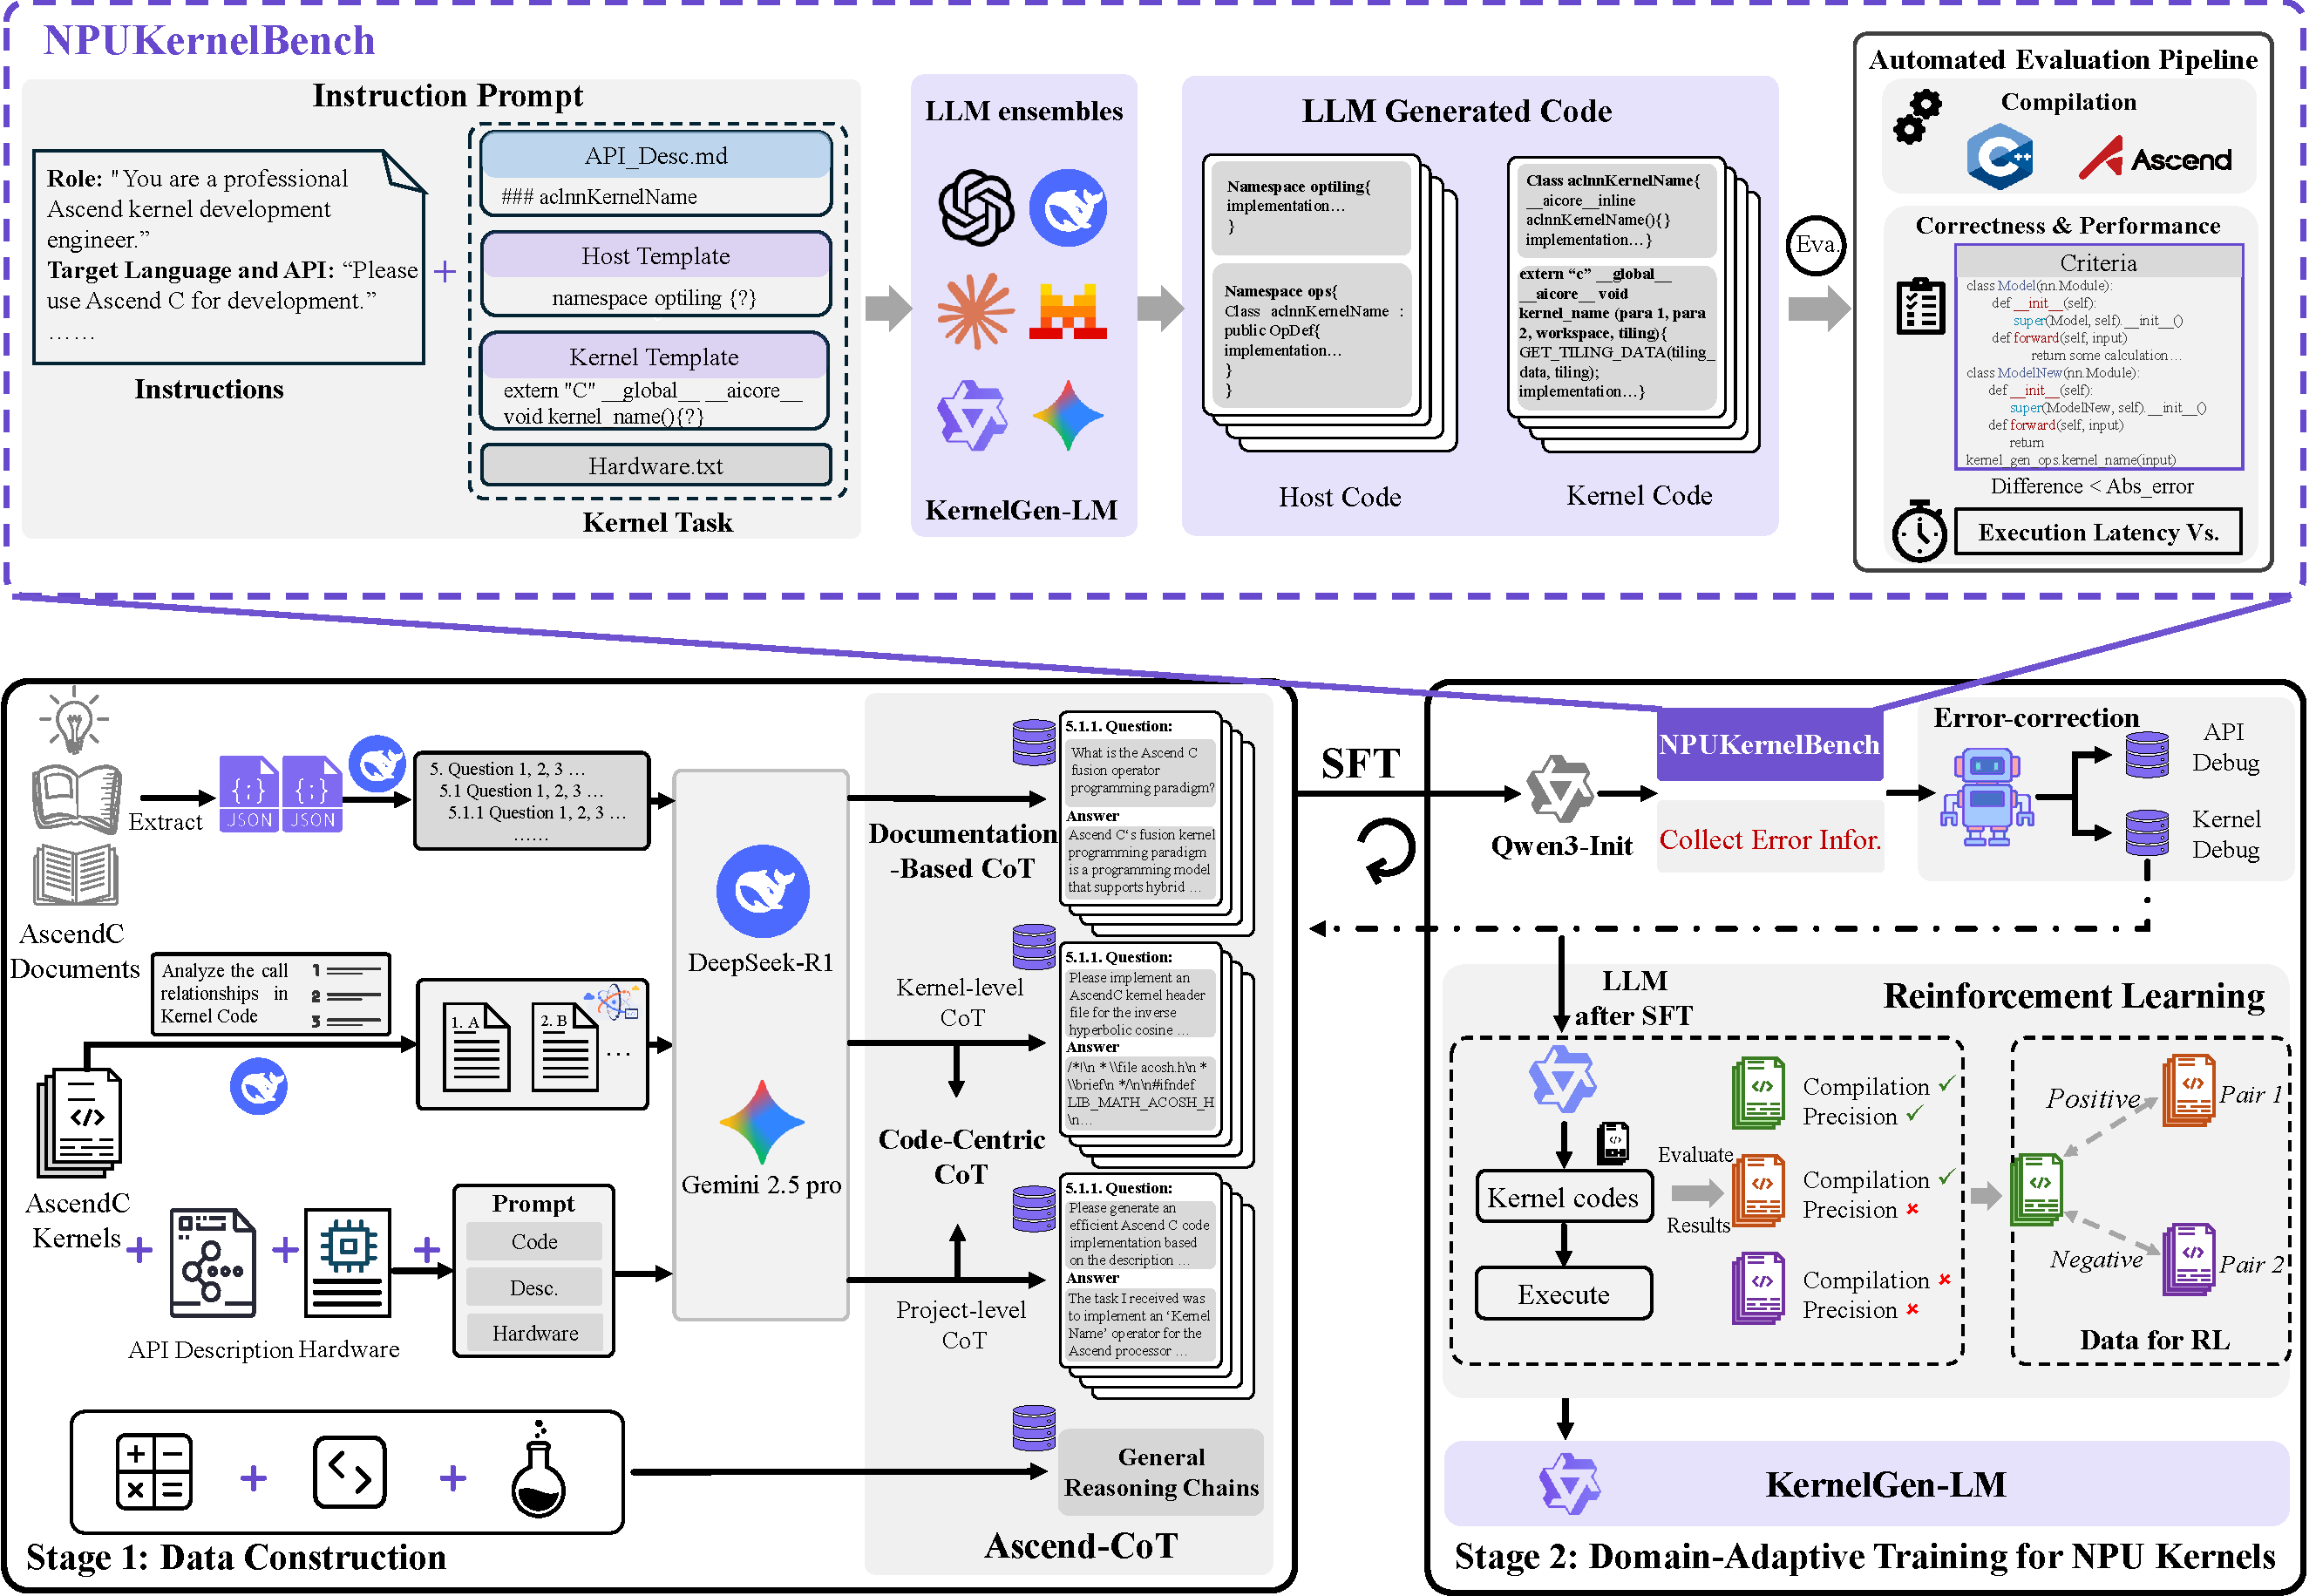
\includegraphics[width=1\linewidth]{pdfs/framework.pdf}
    \caption{System overview of AscendKernelGen, depicting the data construction, LLM training, and hardware-grounded evaluation pipeline for NPU kernel generation.}
    \label{fig:framework}
\end{figure*}

\paragraph{Generation Component.}
The generation side of AKGen is built upon two elements.

\begin{itemize}
    \item \textbf{Ascend Chain-of-Thought Dataset (Ascend-CoT).}
    To address the scarcity of low-level NPU programming data, we construct Ascend-CoT, a curated dataset that captures the structured reasoning processes required for AscendC kernel development. The dataset is collected from real-world operator implementations and documentation, and emphasizes explicit pipeline construction, synchronization logic, and arithmetic reasoning patterns essential to kernel correctness.

    \item \textbf{KernelGen-LM.}
    Using Ascend-CoT, we perform domain-adaptive post-training on a strong base LLM to obtain \textit{KernelGen-LM}, a model specialized for low-level NPU kernel generation. The training objective explicitly targets the reasoning challenges of hardware-aware code generation, including data tiling, asynchronous pipeline orchestration, and correct use of low-level programming interfaces.
\end{itemize}

\begin{comment}

\paragraph{Evaluation Component.}
To systematically assess generated kernels, AKGen incorporates a dedicated evaluation framework, \textit{NPUKernelBench}, which bridges the gap between probabilistic model outputs and deterministic hardware execution.

\begin{itemize}
    \item \textbf{Task Stratification.}
    NPUKernelBench organizes evaluation tasks into multiple difficulty levels, ranging from simple element-wise operators to complex fused kernels. This stratification enables fine-grained analysis of model behavior across diverse computational patterns and levels of programming complexity.

    \item \textbf{Multi-Stage Validation Metrics.}
    Each generated kernel is evaluated through a staged pipeline that checks compilation success, verifies functional correctness against reference implementations, and measures execution performance in terms of runtime. This design isolates distinct failure modes and allows us to quantify model performance beyond surface-level code validity. While the current study emphasizes correctness and performance metrics, the framework is readily extensible to additional analyses such as static code quality and deeper performance characterization.
\end{itemize}

\end{comment}

\paragraph{Evaluation Component.}
To systematically assess generated kernels, AKGen incorporates a dedicated evaluation framework, \textit{NPUKernelBench}, which bridges the gap between probabilistic model outputs and deterministic hardware execution. NPUKernelBench organizes evaluation tasks into multiple difficulty levels, ranging from simple element-wise operators to complex fused kernels, enabling fine-grained analysis of model behavior across diverse computational patterns and levels of programming complexity.

Each generated kernel is evaluated through a staged validation pipeline that checks compilation success, verifies functional correctness against reference implementations, and measures execution performance in terms of runtime. This multi-stage design isolates distinct failure modes and allows us to quantify model behavior beyond surface-level code validity. While the current study emphasizes correctness and performance metrics, the framework is readily extensible to additional analyses, such as static code quality assessment and deeper performance characterization.

Overall, AKGen provides a controlled framework for analyzing how LLMs acquire, apply, and generalize low-level hardware programming knowledge, with Ascend NPU kernels serving as a representative and challenging testbed.

\section{Data Construction}\label{data_construct}

\begin{comment}

\begin{figure}[t]
    \centering
    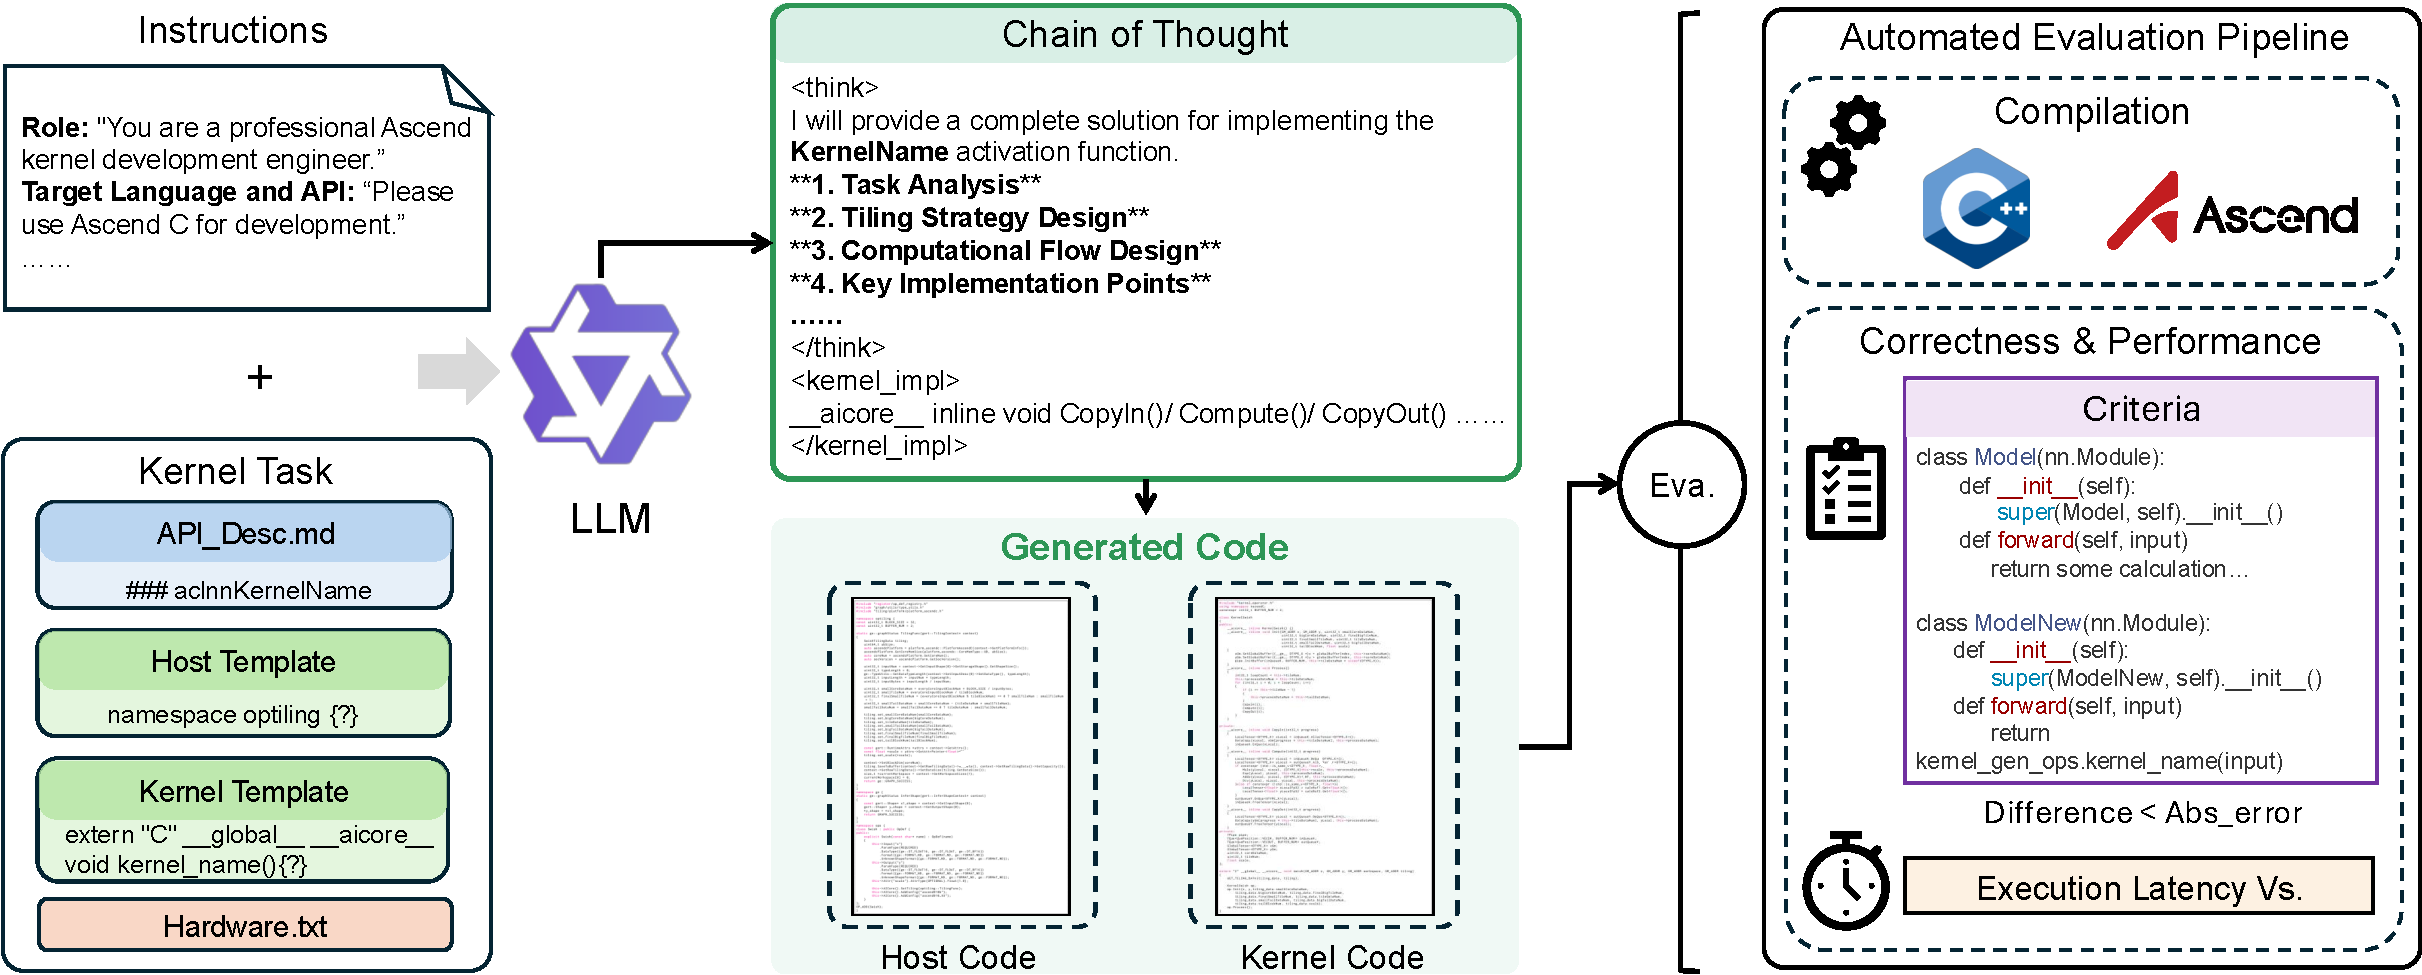
\includegraphics[width=1\linewidth]{pdfs/NPUKernelBench_Overview.pdf}
    \caption{Replace this with data construction figure.}
    \label{fig:Data_Constru}
\end{figure}

% To enable large language models (LLMs) to generate high-quality Huawei Ascend operators, we construct a multi-source dataset integrating both domain-specific and general reasoning data. Specifically, the dataset consists of three complementary components: (1) the \textbf{AscendC Developer Guide}, which provides authoritative and standardized documentation for custom operator development; (2) the \textbf{CANN Kernels}, containing real-world Ascend operator implementations at both single-file and project levels; and (3) the \textbf{General Reasoning Chains}, which includes 100K open-source reasoning traces from the DeepSeek-R1 corpus and high-quality C++ chain-of-thought data. The inclusion of general reasoning data prevents the model from overfitting to domain-specific syntax and ensures that it retains general reasoning and problem-solving abilities.
To enable large language models (LLMs) to generate high-quality Huawei Ascend operators, we construct a multi-source dataset that integrates domain-specific reasoning data with general reasoning data. Specifically, this dataset comprises three complementary components: (1) \textbf{AscendC Documentation Dataset}, which is constructed from official standardized custom operator development documentation to address the issue of models lacking domain knowledge of the Ascend; (2) \textbf{CANN Operator Code Dataset}, which is built from Huawei's open-source Ascend operator libraries (such as Ascend native operators in the MindSpore framework) and publicly available Ascend operator implementations from industry, to address the problem of models understanding functionality but being unable to write code; (3) \textbf{General Reasoning Chain}, which includes 100K open-source reasoning traces from the DeepSeek-R1 corpus and high-quality C++ chain-of-thought data. The inclusion of general reasoning data prevents the model from overfitting to domain-specific syntax and ensures that it retains general reasoning and problem-solving abilities.

\subsection{Ascend C Documentation Dataset}\label{document_dataset}
The Ascend C documentation contains comprehensive domain knowledge of Ascend, such as Ascend's hardware logic, language syntax, API usage, etc. To enable large language models to master the domain knowledge of Ascend C, we use the following three documents to construct the document data:

\textbf{(1) Ascend C Operator Development Guide.} This document introduces the fundamentals of operator development based on the Ascend C operator programming language, including abstract hardware architecture, programming models, etc. It covers both basic concepts for developers to quickly get started and in-depth analysis of core architecture and key technical principles to meet the needs of advanced users for deeper exploration.

\textbf{(2) Ascend C API Documentation.} This document provides a set of library APIs that enable developers to program using standard C++ syntax. The APIs are categorized into Kernel APIs for implementing operator kernel functions (including basic data structures like GlobalTensor and LocalTensor, basic APIs that abstract hardware capabilities, and high-level APIs that implement common computational algorithms), Host APIs (including Tiling APIs for high-level APIs, operator prototype registration and management APIs, Tiling data structure registration APIs, and platform information acquisition APIs), and operator debugging APIs for debugging and performance tuning.

\textbf{(3) Ascend C Best Practices.} This document presents performance optimization strategies, methods, and case studies for Ascend C operators, guiding developers to improve operator performance through an iterative optimization process that includes acquiring performance data, analyzing key performance bottlenecks, designing optimization solutions, and validating performance benefits.

To effectively inject domain knowledge into the model, we develop an automated pipeline that restructures documents into high-quality question-answer pairs with chains of thought reasoning. We adopt the Knowledge-Instruct framework to construct the document dataset in a fully automated manner. Unlike unsupervised continual pre-training (CPT) methods that directly feed entire documents into the base model, our knowledge injection approach significantly improves knowledge retention and mitigates the "hallucination" problem that occurs when small-parameter models learn large amounts of domain-specific knowledge.

\subsubsection{Basic Knowledge QA Data}
To enable large language models to understand domain knowledge of Ascend C, we construct high-quality CoT question-answering data using knowledge documents. Specifically, we first use large language models to generate questions from documents, then employ the RAG paradigm to construct high-quality chains of thought and answers, and perform data augmentation through paraphrasing.

\textbf{(1) Question Generation.} We first segment the documents and use large language models to convert them into JSON format files. Then we use large language models to generate multiple questions for each chapter and section, ensuring that every knowledge point in the document is covered by at least one question. In prompt design, we require the model to ask questions from different cognitive levels, focusing on technical details such as formulas, code, and API usage, while explicitly constraining to avoid duplicate questions and cross-framework content. We also record chapter numbers for subsequent use.

\textbf{(2) Relevant Chapter Retrieval.} We design chapter retrieval prompts to guide the model in locating relevant chapters from the document structure. The prompt follows a "fine-grained priority principle", requiring the model to prioritize selecting the deepest-level and most specific sub-chapters, avoiding the selection of coarse-grained chapters based solely on keyword matching. The model outputs the retrieved chapter IDs along with reasoning for the selection. Based on the retrieved chapter IDs, we load the corresponding document content and concatenate it to form a context-relevant complete prompt. For samples where retrieval fails, we adopt a fallback strategy, directly using the golden chapters recorded during question generation to supplement the context.

\textbf{(3) Chain of Thought and Answer Generation.} We design structured chain of thought generation prompts, requiring the model to output structured content containing both the chain of thought and answer sections. To ensure answer quality, the prompt explicitly prohibits the use of meta-task description terms such as "document", "reference content", and "prompt", making the generated content more natural and fluent. Additionally, we add a paraphrasing step to generate multiple differently-phrased question-answer pairs for the same knowledge point.

\subsubsection{API Call QA Data}
To enable large language models to learn how to call Ascend C API interfaces, we construct high-quality API question-answer pairs with chain-of-thought reasoning using API documentation. Specifically, we first crawl and fix the API documentation from official webpages, then automatically generate high-quality technical question-answer pairs that include a "thinking process" using large language models.

\textbf{(1) Documentation Crawling and Fixing.} To construct high-quality training data, we first need to obtain complete and accurate API documentation. However, the official online documentation presents two major challenges: mathematical formulas are displayed as images and content is scattered across multiple pages. To address this, we developed an intelligent scraping and repair tool that integrates three core technologies: web crawling, OCR recognition, and large language model semantic correction.

The entire process adopts a four-stage pipeline architecture: First, we use Selenium to launch a Headless Chrome browser and parse the documentation entry page to build an API link index. Then, we scrape HTML content page by page and extract plain text context. Next, for formula images in the documentation, we use OpenCV for preprocessing (scaling and binarization to enhance clarity), followed by the pix2tex engine to convert them into preliminary LaTeX code. Finally, we input both the OCR results and page context into the large language model, leveraging its semantic understanding capabilities to fix recognition errors (such as variable name confusion and hallucinated characters). The corrected LaTeX code is inserted into the HTML in \$...\$ format to replace the original image tags, and ultimately converted to Markdown format via markdownify and stored by API category. Through this end-to-end automated process, we successfully converted online documentation containing numerous formula images into high-quality Markdown documents in plain text format, establishing a solid foundation for subsequent question-answer pair generation.

\textbf{(2) Question-Answer Pair Generation.} Building upon the high-quality API documentation obtained after repair, we design an automated question-answer pair generation pipeline. The core of this pipeline leverages the reasoning capabilities of large language models, combined with carefully engineered prompts, to automatically extract and construct high-quality QA data with chain-of-thought reasoning from technical documentation.

For each API document, the system reads the complete content and constructs a structured prompt consisting of three core components: role definition, task constraints, and output format specifications. In prompt design, we emphasize five key requirements: first, the template-first principle, requiring at least one QA pair based on sample code from the documentation; second, complete context, ensuring questions contain all necessary code snippets to be self-contained; third, diversity coverage, asking questions from different dimensions such as parameters, overloads, and constraints; fourth, deep reasoning, requiring simulation of expert thinking processes within `<think>` blocks; fifth, traceability, attaching citations from the original text as evidence.

\subsection{AscendC Kernels}\label{kernel_dataset}
AscendC is a programming language introduced within the CANN Kit specifically for  kernel development scenarios. It follows standard C/C++ conventions and matches developers’ coding habits, while providing multi-layer interface abstractions, automatic parallelization, and twin-mode debugging to significantly improve kernel development efficiency. As part of Huawei’s heterogeneous computing stack, AscendC allows developers to fully exploit the parallel computing capabilities of Huawei’s Da Vinci–architecture NPUs (Neural Processing Units) and other AI-oriented hardware. Although NPUs were originally designed for accelerating deep learning workloads, the CANN software stack—through AscendC and interfaces such as AscendCL—enables developers to implement custom kernels and deploy AI models directly on the NPU with low overhead. This brings substantial acceleration across diverse AI-intensive tasks, including device-side intelligent inference, large-scale training, computer vision, and speech processing.

\begin{wraptable}{r}{0.54\textwidth}
\vspace{-10pt}
\centering
\begin{tcolorbox}[
    rounded corners,
    arc=3pt,
    enhanced,
    width=0.54\textwidth,
    colframe=codegreen, % <----- CHANGED
    colback=white,
    title=\textbf{An example of Kernel Code},
    fonttitle=\bfseries\small,
    boxrule=0.6pt,
    left=2pt,
    right=2pt,
    top=0pt,
    bottom=1pt
  ]
  
\begin{tcolorbox}[
      sharp corners,
      colframe=refgreen,
      colback=refgreen!5,
      colbacktitle=refgreen!15,
      coltitle=refgreen,
      boxrule=0.4pt,
      title={\textbf{Host}},
      fonttitle=\bfseries\small,
      left=0.5pt,
      right=0.5pt,
      top=-5pt,
      bottom=-5pt
    ]
\begin{lstlisting}[style=mystyle, frame=none,framerule=0pt, language=Python]
namespace optiling {
static ge::graphStatus TilingFunc(gert::TilingContext *context)
{ // Initialize tiling data structures and parameter configurations
    TilingData tiling;
    return ge::GRAPH_SUCCESS;
}
} // namespace optiling
namespace ops {
class AddCustom : public OpDef {
public:
    explicit AddCustom(const char *name) : OpDef(name)
    {// Define operator input/output types and computation configuration
    }
};
OP_ADD(AddCustom);
} // namespace ops
\end{lstlisting}
\end{tcolorbox}
\begin{tcolorbox}[
      sharp corners,
      colframe=refgreen,
      colback=refgreen!5,
      colbacktitle=refgreen!15,
      coltitle=refgreen,
      boxrule=0.4pt,
      title={\textbf{Kernel}},
      fonttitle=\bfseries\small,
      left=0.5pt,
      right=0.5pt,
      top=-5pt,
      bottom=-5pt
    ]
\begin{lstlisting}[style=mystyle, frame=none,framerule=0pt, language=Python]
class KernelAdd {
public:
    __aicore__ inline void Init(GM_ADDR x, GM_ADDR y, GM_ADDR z, uint32_t totalLength, uint32_t tileNum) { // Initialize global buffers and queues
    }
    __aicore__ inline void Process() {
        for (int32_t i = 0; i < loopCount; i++) {
            CopyIn(i);
            Compute(i);
            CopyOut(i);
        }
    }
private:
    __aicore__ inline void CopyIn(int32_t progress) {
    // Copy xGm and yGm to local tensors via inQueue
    }
    __aicore__ inline void Compute(int32_t progress) {
    // Dequeue xLocal, yLocal; perform Add; enqueue zLocal
        LocalTensor xLocal = inQueueX.DeQue<DTYPE_X>();
        LocalTensor yLocal = inQueueY.DeQue<DTYPE_Y>();
        LocalTensor zLocal = outQueueZ.AllocTensor<DTYPE_Z>();
        Add(zLocal, xLocal, yLocal, tileLength);
    }
    __aicore__ inline void CopyOut(int32_t progress) {
    // Copy zLocal back to zGm
    }
};
extern "C" __global__ __aicore__ void add_custom(GM_ADDR x, GM_ADDR y, GM_ADDR z) {
    KernelAdd op;
    op.Init(x, y, zzh);
    op.Process();
}
\end{lstlisting}
\end{tcolorbox}
\end{tcolorbox}
\vspace{-15pt}
\captionof{table}{AscendC kernel for vector addition.}
\label{tab:kernel_example}
\vspace{-30pt}
\end{wraptable}

To illustrate the structure of an AscendC operator, we present a complete vector-addition kernel example, shown in Table~\ref{tab:kernel_example}. This example reflects the standard design pattern of custom operators on Huawei Ascend NPUs, where the overall implementation is divided into two tightly coupled components: the \textit{Host-side Tiling implementation} and the \textit{Device-side Kernel implementation}. Together, these two components orchestrate data partitioning, memory transfer, and computation on the AI Core.

\textbf{(1) Host-side Tiling Implementation.}
Because the on-chip memory of Ascend AI Cores cannot store the full input and output tensors, the operator must process data in tiles. The process of partitioning large tensors into smaller chunks and determining how each tile is computed is referred to as \textit{tiling}. The tiling logic—also known as the \textit{tiling strategy} or \textit{Tiling Function}—calculates parameters such as the tile size, the number of iterations, and the memory layout.
Since these computations involve scalar operations and control logic rather than vectorized numerical computation, they are inefficient to execute on the AI Core. Therefore, AscendC places the tiling function on the host side (CPU), where the runtime prepares the tiling metadata and embeds it into a tiling structure that is passed to the device kernel.

\textbf{(2) Device-side Kernel Implementation.}
The device kernel integrates explicit \textit{memory management} and \textit{compute-intensive execution} on the AI Core. To handle the hierarchical memory architecture of Ascend NPUs, input tiles are staged from Global Memory (GM) to on-chip Local Memory (L1/L0) via \texttt{CopyIn()} using DMA queues, while \texttt{CopyOut()} writes results (\texttt{zLocal}) back to GM. This queue-based mechanism decouples data movement from computation, enabling pipelined overlap and high throughput. The core computation runs entirely on the AI Core: local tensors are dequeued (\texttt{inQueueX.DeQue()}, \texttt{inQueueY.DeQue()}), processed via the vectorized \texttt{Add()} intrinsic, and enqueued for output (\texttt{outQueueZ.EnQue()}). Guided by the host-provided tiling metadata, the kernel repeatedly executes this \texttt{CopyIn} → \texttt{Compute} → \texttt{CopyOut} pipeline to complete the operator efficiently.

% \textbf{2) Memory Management.} The Ascend architecture separates \textit{Global Memory (GM)} and \textit{Local Memory (L1/L0)}. Developers must explicitly manage data movement between these memory hierarchies to ensure efficient execution.
% In this kernel, \texttt{CopyIn()} transfers input data (\texttt{xGm}, \texttt{yGm}) from GM to local tensors (\texttt{xLocal}, \texttt{yLocal}); \texttt{Compute()} performs the addition on local tensors; and \texttt{CopyOut()} writes the computed result (\texttt{zLocal}) back to GM.
% Data transfers are handled via DMA queues, enabling pipelined overlap between communication and computation.

% \textbf{3) Device (AI Core) Kernel.} The core computation runs on the AI Core, where the operator executes in a pipelined manner. The queue mechanism decouples data movement and computation to improve throughput. During each iteration, \texttt{inQueueX.DeQue()} and \texttt{inQueueY.DeQue()} fetch local tensors, \texttt{Add()} performs element-wise addition, and \texttt{outQueueZ.EnQue()} pushes results to the output queue for write-back.

The overall process includes: (1) the host computes the tiling strategy, determines tile sizes and loop counts, and allocates GM buffers; (2) the runtime launches the kernel on the AI Core, passing GM addresses and tiling metadata; (3) \texttt{Init()} sets up local buffers, queue descriptors, and other resources based on the tiling configuration; (4) \texttt{Process()} executes tile-wise pipelined computation, where \texttt{CopyIn} transfers input tiles from GM to Local Memory, \texttt{Compute} performs vectorized addition on local tensors (\texttt{inQueueX.DeQue()}, \texttt{inQueueY.DeQue()}, \texttt{Add()}), and \texttt{CopyOut} writes results back to GM (\texttt{outQueueZ.EnQue()}); and (5) the host retrieves the final results from GM for validation.

\subsubsection{Single-File CoT Construction}\label{single_file}
This section aims to enable the LLM to learn kernel grammar by constructing high-quality code chain-of-thought from a single kernel file that can be compiled without errors. To achieve this, we follow a three-step pipeline: we first generate questions based on the given kernel code, then construct well-structured question–answer (QA) pairs that serve as the basis for reasoning, and finally feed these QA pairs into the LLM to produce detailed chain-of-thought explanations that guide the generation of correct answer code. 

\textbf{(1) Generating Question.}
To generate a question for each kernel file, we first analyze the internal call relationships to identify all dependent files. Based on this analysis, we reorganize the target file together with its dependencies into a single, self-contained code snippet that can be compiled without errors. This consolidated snippet is then provided—along with its dependency code—as input to the LLM, together with the prompt specified in Table~\ref{tab:prompt_single_file_qa}, to guide the LLM in generating a question that accurately reflects the code’s functionality.

\begin{wraptable}{l}{0.5\textwidth}
\vspace{-20pt}
\centering
\begin{tcolorbox}[
    sharp corners,
      colframe=reforange,
      colback=reforange!5,
      colbacktitle=reforange!15,
      coltitle=reforange,
      boxrule=0.4pt,
      title={\textbf{Prompt for generating question}},
      fonttitle=\bfseries\small,
      left=0.5pt,
      right=0.5pt,
      top=0.5pt,
      bottom=0.5pt
]
{\small
You are an expert in AscendC programming for the Huawei Ascend processor. Based on the provided answer code, please generate a corresponding request for that code.

\textbf{Background:} 

I maintain an AscendC operator repository that contains many operators, and each operator consists of multiple code files. I am constructing a dataset to train an LLM that can assist in writing AscendC operators. Each file within an operator will serve as a single training sample. I already have the answer code for each sample, but I still need to generate the corresponding request. After I provide you with a piece of answer code, your task is to analyze the code, understand and summarize its purpose, and then generate a request such that the provided code naturally serves as a correct response to that request. The request should be high-level and concise rather than overly detailed.

Please output the request in the following format:

\verb|<request>REQUEST_TEXT</request>| 

Note: Output only the final request—no reasoning process.

\textbf{Requirements:}

1. The request must capture the core functionality and purpose of the code.

2. The request should be clear and concise, avoiding unnecessary complexity.

The answer code is provided below:

[ ... Kernel code ... ]

}
\end{tcolorbox}
% \begin{tcolorbox}[
%     sharp corners,
%       colframe=reforange,
%       colback=reforange!5,
%       colbacktitle=reforange!15,
%       coltitle=reforange,
%       boxrule=0.4pt,
%       title={\textbf{Generated question samples}},
%       fonttitle=\bfseries\small,
%       left=0.5pt,
%       right=0.5pt,
%       top=0.5pt,
%       bottom=0.5pt
% ]
% {\small
% <request> Please create an interface header file for the Sigmoid operator that includes the required header references, uses the AscendC namespace, and provides a deprecation notice pointing to the new sigmoid.h file. </request>

% <request> Please implement an AscendC operator header file that defines the computation interface for the Swish activation function. The activation is defined as swish$(x) = x / (1 + e^{(-βx)})$, and it should support both half and float data types. </request>
% }
% \end{tcolorbox}
\vspace{-15pt}
\captionof{table}{Prompt for generating question.}
\label{tab:prompt_single_file_qa}
\vspace{-100pt}
\end{wraptable}



Examples of the generated questions include:

\noindent\parbox{\linewidth}{
\small
\texttt{<request> Please create an interface header file for the Sigmoid operator that includes the required header references, uses the AscendC namespace, and provides a deprecation notice pointing to the new sigmoid.h file. </request>}
}
\parbox{\linewidth}{
\small
\texttt{<request> Please implement an AscendC operator header file that defines the computation interface for the Swish activation function. The activation is defined as swish$(x) = x / (1 + e^{(-βx)})$, and it should support both half and float data types. </request>}
}

\textbf{(2) Constructing Standard QA Pairs.} Building on the questions generated in Step (1), we then construct standard question–answer (QA) pairs to guide the LLM and facilitate chain-of-thought (CoT) reasoning. Each QA pair corresponds to a single self-contained code snippet. In particular, the question includes both (i) the question describing the intended functionality and (ii) all necessary dependency code that the answer must incorporate. The answer then provides the complete implementation of the requested functionality.
By jointly packaging the request and its relevant dependencies into the question and pairing them with the correct implementation, we form high-quality training samples that precisely reflect the mapping from problem statements to valid code solutions. Examples of these QA pairs are provided in the Appendix.

\textbf{(3) Generating Code-centric CoT.}
After constructing the QA pairs, we feed the constructed QA pairs into the LLM to generate kernel-centric CoT reasoning. Each QA pair produces a corresponding reasoning trace, which is further organized into a unified JSON format for downstream use. Through this pipeline, we obtain over 7k high-quality kernel-centric CoT samples, forming a substantial and diverse dataset for supervised training. A full example of the generated CoT is provided in Table \ref{tab:singel_example} the Appendix.


\subsubsection{Project-level CoT Construction}\label{project_file}
This section aims to enable the LLM to generate a complete kernel. To achieve this goal, we first need to construct high-quality Chain-of-Thought (CoT) documents from Ascend C kernel source code, test cases, and hardware specifications, which guide Host-side tiling parameter computation and Kernel-side pipeline design, and are later verified and optimized. However, industrial-grade Ascend C operators are typically large composite files with numerous shape branches, data types, and hardware-specific logic, resulting in low signal-to-noise ratios and often exceeding the context window of large models. To address this difficulty, we develop an intelligent deconstruction pipeline that breaks down a complex composite operator into multiple clean Host-Kernel code pairs and automatically generates the corresponding API documentation. Based on this foundation, the overall workflow proceeds as follows: (1) decomposing the composite operator into logically pure one-to-one Host-Kernel pairs; (2) constructing prompts by integrating kernel code, test cases, and hardware configurations; (3) feeding the combined prompt into the LLM to generate kernel-centric CoT; and (4) verifying and selecting high-quality CoT files according to execution results.

\textbf{(1) Host-Kernel Decomposition.}
Industrial-grade AscendC kernels are typically composite structures that embed multiple Shapes, Dtypes, and hardware modes within deeply nested templates and conditional branches. Such complexity results in low signal-to-noise ratios and makes the code unsuitable as direct input for LLM. To address this, we design a Host–Kernel collaborative decomposition pipeline:
\begin{itemize}
    \item Kernel-side extraction. All mutually exclusive execution paths (e.g., float16, float32, int8) are identified and extracted into independent, logically pure Kernel fragments. Each fragment is associated with a unique tiling key representing the conditions that trigger its execution.
    \item Host-side pruning. Using the tiling key, only the Host-side branches required to generate that key are retained, producing a streamlined Host fragment that aligns precisely with the corresponding Kernel logic.
    \item Atomic sample construction. Each data scenario is thereby decomposed into a pair of noise-free Host–Kernel atomic samples, providing clean and contextually consistent inputs for CoT generation and model training.
\end{itemize}
Table \ref{tab:kernel_host_decompos} compares the operator structure before and after decoupling. After decoupling, each data scenario is mapped to its own isolated and self-contained Host–Kernel code pair.
\begin{table}[t]
\begin{tcolorbox}[
sharp corners,
      colframe=refgreen,
      colback=refgreen!5,
      colbacktitle=refgreen!15,
      coltitle=refgreen,
      boxrule=0.4pt,
      title={\textbf{Host-Kernel Decomposition}},
      fonttitle=\bfseries\small,
      top=-10pt, bottom=0pt, left=1pt, right=1pt
]
\begin{tabular}{p{0.48\textwidth} p{0.48\textwidth}}
\begin{lstlisting}[basicstyle=\ttfamily\scriptsize]
# Before decomposing
.../{op_name}/answer/
+-- 0/
    |-- op_host/
    |   |-- add_custom.h
    |   `-- add_custom.cpp
    `-- op_kernel/
        |-- add_custom.h
        `-- add_custom.cpp
\end{lstlisting}
&
\begin{lstlisting}[basicstyle=\ttfamily\scriptsize]
# After decomposing
.../{op_name}/answer/
+-- 0/
|   +-- ... (Original backup)
+-- 1/
|   +-- op_host/ (<- The Host code of scenario 1.)
|   |   +-- add_custom.h
|   |   `-- add_custom.cpp
|   +-- op_kernel/
|   |   +-- add_custom.h
|   |   `-- add_custom.cpp
|   `-- tiling_key.json
`-- 2/
    +-- op_host/ (<- The Host code of scenario 2.)
    |   +-- add_custom.h
    |   `-- add_custom.cpp
    +-- op_kernel/
    |   +-- add_custom.h
    |   `-- add_custom.cpp
    `-- tiling_key.json
\end{lstlisting}
\end{tabular}
\end{tcolorbox}
\caption{The kernel code structure before and after decoupling. }
\label{tab:kernel_host_decompos}
\end{table}

\textbf{(2) Constructing Prompt.}
To effectively guide the LLM in generating a complete kernel project, it is necessary to construct CoT at the project level for supervised finetuning. Consequently, prior to formulating the CoT, we first design the prompt that will serve as its structural basis. In particular, the prompt is composed of four elements: the instruction text, kernel source code, test cases, and NPU hardware configuration. These components are then concatenated in a predefined order, thereby forming a single, coherent input file that is subsequently provided to the model. The full prompt specification is presented in Table~\ref{tab:prompt_project_file} in the Appendix.


\textbf{(3) Generating Kernel-centric CoT.}
After constructing the prompt, we feed it to the LLM to generate the kernel-centric CoT. In particular, the “thinking” component encompasses both the design of host-side tiling strategies and the implementation and pipeline design on the kernel side. Moreover, we also output a JSON summary containing all tiling parameter values following the generated thought chain. This summary is subsequently used to evaluate the quality of the CoT in the following sections. The generated CoT example is presented in Table~\ref{tab:prompt_project_file} in the Appendix.

\textbf{(4) CoT Verification and Optimization.}
To ensure high-quality CoTs, we perform two sequential steps:
\textbf{(a) Verification.} We first verify correctness by comparing the tiling JSON generated in Step (3) against predefined Gold Standard Logs, thereby validating the accuracy of the inferred tiling parameters.
\textbf{(b) Optimization.} Since the initial CoTs contain substantial redundant summarization that obscures core reasoning, we then refine only those CoTs that pass verification. Specifically, We automatically simplify their content to remove redundancy and highlight the essential tiling and pipelined reasoning steps. This is achieved using a tailored System Prompt that defines the LLM as a CoT optimization expert, together with a User Prompt specifying the optimization goals and modification rules. The complete prompts are provided in Table~\ref{tab:optimization_prompt}. This two-stage process ensures that the final CoTs are both reliable and well structured for subsequent evaluations.



\subsection{General Reasoning Chains}
% At the mean time, we also 

% Integrating explicit domain knowledge, whether through structured prompting or targeted fine-tuning, can significantly enhance the capability of LLMs in domain-specific code generation, including specialized tasks such as kernel development.
Leveraging the CoT datasets constructed in Sec.~\ref{kernel_dataset} and Sec.~\ref{document_dataset}, we fine-tune the LLM to better handle domain-specific kernel generation. However, relying exclusively on kernel-oriented data risks catastrophic forgetting. To balance specialization and generality, we incorporate several open-source CoT datasets~\cite{Chinese-Data-Distill-From-R1,AM-DeepSeek-R1-0528-Distilled,r1-dataset-collection-2025,reasoning_gemini_300k_2025}, including Chinese-Deepseek-R1-Distill-data-110k, AM-deepseek-R1-0528-Distilled, math-code-science-deepseek-r1-en, and reasoning\_gemini\_300k.

To ensure high-quality and consistent supervision across heterogeneous sources, we apply a unified cleaning pipeline with the following steps:

\textbf{(1) Language filtering and normalization.}
\begin{itemize}
    \item We remove samples written in low-resource languages, convert Traditional Chinese to Simplified Chinese, and enforce language ratios specific to each type of data: 5\% Chinese / 95\% English for code-related samples, and 50\% Chinese / 50\% English for math-related or code–math hybrid samples.
\end{itemize}


\textbf{(2) Task-specific filtering.}
\begin{itemize}
    \item Code-related samples: retain only samples with code length greater than 2k tokens and perplexity (if available) below 3.5;
    \item Math-related or code–math hybrid samples: retain only samples longer than 1.5k tokens with perplexity (if available) below 3.5.
\end{itemize}
This pipeline ensures that the resulting dataset is clean, balanced, and suitable for both general reasoning and domain-specific code or math tasks.

% To ensure data quality, we further perform a thorough cleaning process.
% First, we filter out CoT samples written in low-resource languages.
% Second, for code-related data, we retain only samples whose code length exceeds 2 and whose perplexity (when available) is below 3.5. We convert Traditional Chinese to Simplified Chinese and maintain an overall ratio of 5\% Chinese to 95\% English.
% Finally, for code-related data, we keep samples longer than 1.5k tokens with perplexity (if available) below 3.5, ensuring a 50\%-Chinese / 50\%-English balance.

% \subsubsection{Open-Source CoT Dataset}



% \subsubsection{high-quality C++ Cot Samples}

\end{comment}

%\begin{comment}

To equip large language models (LLMs) with the reasoning capabilities required for low-level NPU kernel generation, we construct a multi-source dataset that integrates domain-specific kernel knowledge with general reasoning supervision. The design goal is not only to expose the model to the surface form of AscendC kernels, but also to teach how expert developers reason about tiling strategies, memory movement, API constraints, and correctness under hardware-specific execution models.

As illustrated in Fig.~\ref{fig:framework}, the dataset consists of three complementary components: documentation-based reasoning data derived from AscendC manuals, kernel-centric chain-of-thought (CoT) data extracted from real-world AscendC operators, and general reasoning chains to preserve generalization capability. In total, the raw corpus contains 83,916 samples and is publicly available at \href{https://huggingface.co/AscendKernelGen/datasets}{\textcolor{blue}{Ascend-CoT}}.

The raw dataset exhibits a long-tailed length distribution. Approximately 99.1\% of samples have input sequences shorter than 11.1k tokens, although the maximum input length reaches about 111k tokens. On the output side, 85.1\% of samples are within 21.9k tokens and an additional 6.3\% fall between 21.9k and 43.8k tokens, while the maximum output length reaches about 219k tokens. Before supervised fine-tuning, we apply length-aware preprocessing: samples exceeding 32k tokens are discarded, and short samples are packed into fixed-length training sequences using boundary-aware isolation to prevent interference across concatenated examples. After preprocessing, the final SFT corpus consists of 9,955 sequences of length 32k.

\subsection{Documentation-Based CoT Data}
\label{document_dataset}

The AscendC programming ecosystem contains rich but highly specialized knowledge spanning hardware abstractions, programming models, and low-level API semantics. To inject this domain knowledge into LLMs in a controllable manner, we transform official AscendC documentation into structured, reasoning-oriented supervision rather than treating it as unstructured text.

Specifically, we construct documentation-based supervision from three authoritative sources: the AscendC Operator Development Guide, which introduces hardware abstractions and the programming model; the AscendC API Reference, which specifies kernel, host, and debugging interfaces; and the AscendC Best Practices, which describe performance optimization strategies and common pitfalls. Together, these sources provide comprehensive coverage of both functional correctness and performance-oriented considerations.

Instead of unsupervised continual pre-training, we adopt a \emph{knowledge-instruct} paradigm that converts documentation content into question–-answer pairs augmented with explicit reasoning traces. The resulting supervision emphasizes not only factual knowledge of APIs and concepts, but also the reasoning process underlying correct API usage and constraint satisfaction. This design mitigates hallucination caused by shallow pattern memorization and encourages systematic reasoning about hardware and programming constraints.

The constructed documentation-based dataset covers both conceptual reasoning over hardware abstractions and programming semantics, as well as API-centric reasoning that focuses on invocation patterns, parameter constraints, and typical error scenarios. Each sample consists of a natural-language question, a structured chain of reasoning, and a grounded answer. To ensure coverage and diversity, we enforce fine-grained chapter alignment and apply paraphrase augmentation during data generation.

\begin{comment}

\paragraph{Basic Knowledge and API Reasoning QA.}
From the documentation, we automatically construct two types of supervision:
\begin{itemize}
    \item Conceptual reasoning QA, which focuses on hardware concepts, programming models, and execution semantics;
    \item API-centric reasoning QA, which teaches correct API invocation patterns, parameter constraints, and typical error scenarios.
\end{itemize}

Each sample contains a natural-language question, a structured chain of reasoning, and a grounded answer. To ensure coverage and diversity, we enforce fine-grained chapter alignment and paraphrase augmentation during generation.

\end{comment}

\subsection{Code-Centric CoT Data}
\label{kernel_dataset}

Beyond documentation, correct kernel generation requires understanding how host-side tiling logic interacts with device-side kernel execution in practice. To capture this interaction, we construct code-centric chain-of-thought (CoT) data from real-world AscendC operator implementations.

For standalone kernel files that can be compiled independently, we generate kernel-level CoT samples that explicitly explain kernel structure, memory movement, and computation logic. Each sample pairs a functional specification with a complete kernel implementation and an explicit reasoning trace that justifies key design decisions, such as tiling assumptions, buffer usage, and pipeline organization.

However, industrial-grade AscendC operators are typically implemented as composite projects that support multiple shapes, data types, and execution branches. These implementations interleave host-side tiling logic with device-side kernel invocation, making them unsuitable for direct supervision. To address this challenge, we systematically decompose complex operators into logically pure host--kernel pairs, where each pair corresponds to a single execution scenario with fixed tiling and shape assumptions.

For each decomposed host--kernel pair, we construct project-level CoT supervision that jointly reasons about host-side tiling parameter computation, kernel-side pipeline structure and memory staging, and the consistency between tiling metadata and kernel execution behavior. This joint reasoning explicitly exposes the cross-boundary dependencies that are essential for correct kernel generation but are rarely visible in isolated kernel code.

To ensure correctness and executability, we retain only CoT samples that pass automated verification against reference tiling configurations. This filtering step guarantees that the generated reasoning traces are not only conceptually coherent but also aligned with valid host--kernel execution semantics.

\begin{comment}

\paragraph{Single-File Kernel Reasoning.}
For standalone kernel files that compile independently, we generate code-centric CoT samples that explain kernel structure, memory movement, and computation logic. Each sample pairs a functional specification with a complete implementation and an explicit reasoning trace that justifies design decisions.

\paragraph{Project-Level Kernel Reasoning.}
Industrial-grade AscendC operators are often implemented as large composite projects with multiple shapes, data types, and execution branches, making them unsuitable for direct supervision. To address this, we decompose complex operators into logically pure host–kernel pairs, each corresponding to a single execution scenario.

For each decomposed Host--Kernel pair, we construct project-level CoT supervision that jointly reasons about host-side tiling parameter computation, kernel-side pipeline structure and memory staging, as well as the consistency between tiling metadata and kernel execution.

Only CoT samples that pass automated verification against reference tiling configurations are retained, ensuring that the reasoning traces are both correct and executable.

\end{comment}

\subsection{General CoT Data}
\label{general_cot}

While domain-specific supervision is essential, training exclusively on kernel data risks degrading general reasoning ability. To balance specialization and generality, we augment our dataset with high-quality open-source chain-of-thought corpora covering mathematics, code reasoning, and scientific problem solving~\cite{Chinese-Data-Distill-From-R1,AM-DeepSeek-R1-0528-Distilled,r1-dataset-collection-2025,reasoning_gemini_300k_2025}.

We apply a unified filtering and normalization pipeline to ensure consistency across heterogeneous sources, including language normalization, length-based filtering, and perplexity-based quality control. This mixture allows the model to retain general problem-solving skills while adapting to the highly specialized reasoning demands of NPU kernel generation.

%\end{comment}
\section{LLM Fine-Tuning for NPU Kernels}\label{fine_tune}
% 描述ft的目的和分两步走实现的策略
% 章节5中介绍了数据集，下面我们利用SFT和RL来注入领域知识。在SFT中, 除了使用到上一章节我们构建的数据集外，我们还使用了数据飞轮的操作。具体来说我们大量的报错信息进行了数据纠正xxx。与此同时，我们还使用了强化学习来增加AscendC 的领域知识，其中我们利用SFT生成大量的算子实例，并根据算子的执行结果（编译，精度通过情况）进行评估，自动构建用于训练的正负样本对。

%我们通过两个步骤来增强LLM生成AscendC算子的能力。分别是基于基于Ascend知识增强的SFT和强化学习。在SFT知识注入后，我们还设计了一套针对算子精度问题的高质量SFT训练数据，通过处理那些SFT之后“编译通过但运行结果错误”的高难度样本，结合GT标准答案，引导大模型进行深度归因分析和从零重构。在强化学习中，我们通过对SFT之后的测试算子样例的执行结果（编译，精度通过情况）进行评估，自动构建用于训练的正负样本对。
%We enhance the LLM’s ability to generate AscendC kernels through two steps: (1) Ascend-knowledge–augmented supervised fine-tuning (SFT) and (2) reinforcement learning (RL). In the first step, we perform Ascend-specific SFT using the curated dataset described in Sec.~\ref{data_construct}. We then apply a data-flywheel: we collect challenging cases that compile but fail precision tests, pair them with ground-truth references, and use them to guide the LLM in causal analysis and reconstruction. In the second step, building on the improved SFT model, we generate a large number of kernel instances and automatically construct positive–negative training pairs based on compilation and precision results, enabling RL to further refine the model in a robust and correctness-oriented manner.

To enable reliable NPU kernel generation under strict programming constraints, we introduce \href{https://huggingface.co/AscendKernelGen/models}{\textcolor{blue}{KernelGen-LM}}, a publicly available domain-adapted model designed to internalize AscendC-specific API semantics and complex execution dependencies. Our approach employs a two-stage optimization strategy combining Supervised Fine-Tuning (SFT) and Reinforcement Learning (RL). The first stage performs NPU-aware supervised fine-tuning (SFT) with curated and iteratively refined data, enabling the model to acquire foundational knowledge of AscendC syntax, APIs, and kernel structure. The second stage further refines the model via reinforcement learning (RL) using execution-based correctness signals, encouraging the generation of kernels that are not only compilable but also numerically correct.

\subsection{Supervised Fine-Tuning with Error-Derived Supervision}

%Since the original LLM lacks AscendC knowledge for NPU kernel generation, we first construct a carefully designed dataset (see Sec.~\ref{data_construct}) to provide instruction through supervised fine-tuning (SFT). However, even after knowledge injection, the model is not yet ready for reinforcement learning due to suboptimal compilation success and computational accuracy. To address this, we perform framework-level verification on generated kernels to collect error logs, revealing the model’s limitations. We then establish an interaction mechanism between the LLM and the compilation framework to systematically identify deficiencies, generate targeted error-correction training data, and incorporate it into the pretraining dataset. This iterative process forms a data flywheel that progressively improves model performance, integrating retrieval-based augmentation from the AscendC API with kernel-level error-correction optimization.
While Ascend-aware SFT provides essential syntactic and structural knowledge, we observe that models trained solely on static supervision still exhibit frequent failures in compilation stability and numerical correctness. To improve robustness prior to RL, we introduce an \emph{error-derived supervision} strategy that augments SFT with correction data generated from real execution failures, shown in Figure~\ref{fig:error_correction}. 
\begin{wrapfigure}{l}{0.48\linewidth}
    \centering
    % \vspace{-10pt}
    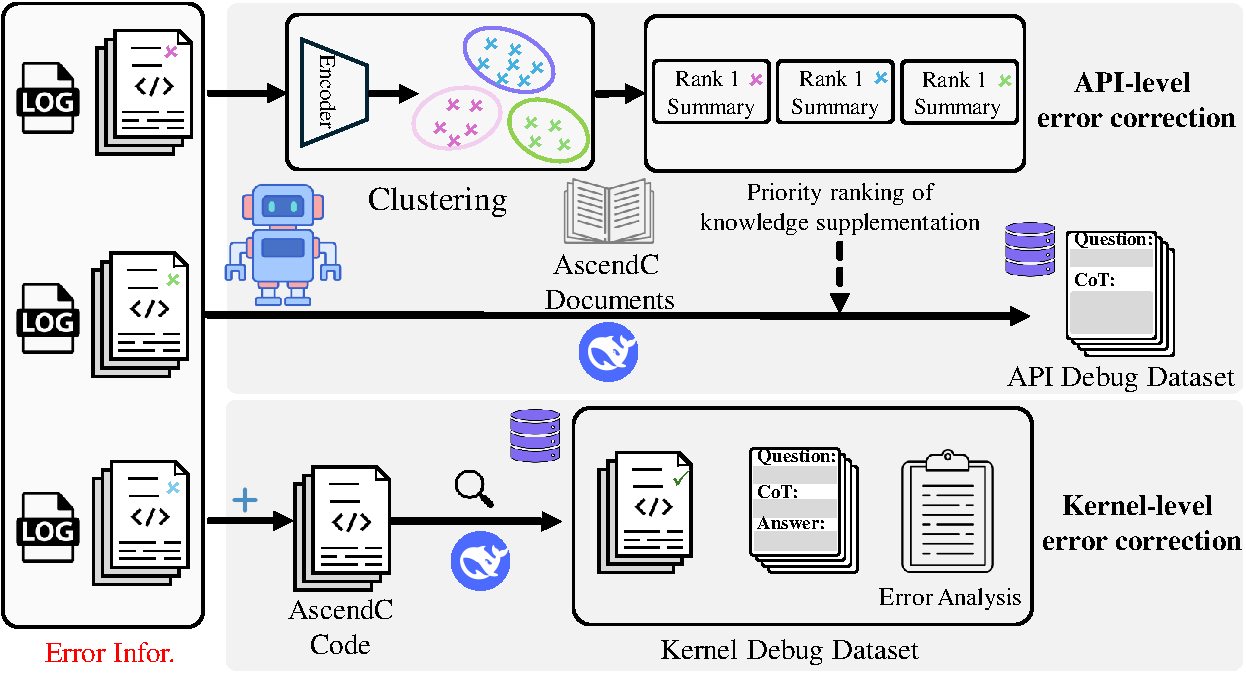
\includegraphics[width=\linewidth]{pdfs/data_debug.pdf}
    \caption{Error-Derived Supervision for API- and Kernel-Level Error Correction.}
    \vspace{-10pt}
    \label{fig:error_correction}
\end{wrapfigure}
This strategy focuses on two complementary levels of errors: API-level misuse and kernel-level numerical inconsistency.

\begin{comment}

To address this limitation, we introduce an \emph{error-derived supervision} mechanism integrated into the SFT process. Kernel generation and verification are treated as an offline data augmentation pipeline: kernels produced by the current SFT model are compiled and executed using an automatic verifier, and failure cases are systematically collected and analyzed. Execution errors, including API misuse, invalid tiling logic, and numerical inaccuracies, are transformed into structured correction examples that explicitly demonstrate the correct behavior.

This process remains fully supervised. Each newly generated sample is paired with a deterministic ground-truth target, such as corrected API invocations or reference kernel implementations, and is incorporated back into the training corpus for subsequent SFT iterations. By iteratively exposing the model to its own failure modes and providing explicit corrective supervision, the model progressively internalizes execution constraints and kernel-level invariants that are difficult to encode a priori through static data alone.

\end{comment}


%知识注入后的模型在效果上尚未达到可启动强化学习的门槛，主要表现为编译通过率与计算精度达标率仍不够理想。通过对生成算子进行框架侧验证，我们能够获取大量报错信息，这些信息清晰地揭示了模型当前的能力短板。为此，我们尝试建立模型与编译框架之间的交互机制：通过系统化识别模型缺陷，自动合成针对性的改错训练数据，并将其加入模型的预训练数据集。通过这一方式，我们正逐步构建起能够持续优化模型性能的数据飞轮


\subsubsection{API-Level Error Correction}
\label{sft_api_correction}

% Despite having constructed API invocation QA data, large language models still exhibit invocation errors, leading to high operator compilation failure rates. Therefore, we built an automated data generation pipeline to transform Ascend C operator compilation failure logs into high-quality API code debugging SFT training data. This pipeline integrates raw error logs, operator source code context, and official API documentation to automatically generate structured training samples containing "error scene + expert reasoning process + correct documentation references." The entire data construction process adopts a modular four-stage architecture, with each stage focusing on specific data transformation tasks:

% \textbf{(1) Log cleaning and extraction.} This stage filters clean error information from mixed build logs. Through regular expression matching of [ERROR] marker blocks, it automatically removes successfully compiled samples and stores error logs in a flattened structure, establishing a clean data foundation for subsequent analysis.

% \textbf{(2) Error analysis and strategic filtering.} This stage utilizes large language models for root cause analysis and error type classification, while identifying "low-pass-rate" difficult operators by calculating operator compilation pass rates. This dual filtering mechanism ensures subsequent processing focuses on the most challenging and valuable training samples.

% \textbf{(3) Contextual diagnostic report generation.} This is the core stage of the entire pipeline. The system automatically correlates three types of information sources: 1) specific error messages from error logs; 2) erroneous invocations and their context in source code (including variable definition backtracing); 3) correct usage instructions from official API documentation. These three elements are physically concatenated to form structured Markdown diagnostic reports, providing complete problem scenes for expert-level reasoning.

% \textbf{(4) SFT data synthesis.} Based on diagnostic reports, large language models act as domain experts to generate high-quality conversational data containing chain-of-thought reasoning. The system automatically performs data balancing (downsampling high-frequency errors) and data augmentation (generating diverse phrasings for low-frequency errors), and filters out invalid samples with insufficient information.

At the API level, we construct an error-correction dataset from real AscendC compilation failures. Given a compiler error log, the corresponding kernel context, and relevant official documentation, the model is trained to identify the root cause of the failure and produce a corrected implementation. This supervision explicitly targets a common failure mode of LLM-based kernel generation, where API invocations are syntactically plausible but violate semantic constraints or usage requirements.

The overall construction process is summarized in Algorithm~\ref{alg:api_sft_pipeline}, which formalizes how compilation errors are analyzed and transformed into supervised correction examples.

\begin{algorithm}[t]
\caption{Workflow for Constructing Ascend C API Correction SFT Data}
\label{alg:api_sft_pipeline}

\KwIn{
  Raw build logs; \\
  Source-code repository; \\
  OCR-extracted API documentation
}
\KwOut{SFT dataset with reasoning and corrected API usage}

% ----------- Step 1 -----------
\textbf{Step 1: Extract Error Logs} \\
\Begin{
  Traverse all build logs; \\
  \ForEach{log file}{
    \If{contains error messages}{
      Extract the error block and save it as a clean error sample;
    }
  }
}

\vspace{1mm}

% ----------- Step 2 / Step 3.0 -----------
\textbf{Step 2: Error Distribution Analysis} \\
\Begin{
  Classify error types using an LLM; \\
  Compute pass/fail statistics to identify challenging operators; \\
  Optionally filter easy cases using the statistics.
}

\vspace{1mm}

% ----------- Step 3.1 -----------
\textbf{Step 3: Contextual Diagnostic Report Generation} \\
\Begin{
  \ForEach{error sample}{
    Retrieve related code snippet and variable definitions; \\
    Retrieve the corresponding API documentation; \\
    Merge log excerpt, code context, and API reference into a structured Markdown report;
  }
}

\vspace{1mm}

% ----------- Step 4 -----------
\textbf{Step 4: SFT Data Synthesis} \\
\Begin{
  \ForEach{diagnostic report}{
    Prompt an LLM to: \\
    \Indp analyze the misuse of the API; \\
    produce expert reasoning (\texttt{<think>}); \\
    propose corrected usage and explanations; \Indm \\
    Save the result as an SFT training instance;
  }

  Apply data balancing via subsampling or augmentation; \\
  Remove low-quality or incomplete samples.
}

\end{algorithm}


\subsubsection{Kernel-Level Error Correction}\label{sft_kernel_correction}

%Although we have generated high-quality Single-file and project-level CoTs for SFT, we observed that the LLM may still produce high-difficulty kernels that compile successfully but exhibit precision errors. This indicates that, while the existing SFT data effectively guides the model for general kernel codes, it is insufficient for challenging kernels that require deeper reasoning about subtle kernel-level behaviors. To address this limitation, we introduce a pipeline that leverages ground-truth (GT) kernel implementations to guide the model in performing root-cause analysis and reconstructing kernels from scratch.

Beyond compilation errors, a substantial fraction of generated kernels compile successfully but fail numerical verification. Such failures typically arise from subtle kernel-level reasoning issues, including incorrect memory staging, accumulation order mismatches, or inconsistencies between host-side tiling metadata and device-side execution logic.

To address these errors within the supervised learning paradigm, we construct ground-truth–-guided reconstruction data. As formalized in Algorithm~\ref{alg:precision_sft_pipeline}, kernels that pass compilation but fail numerical verification are first identified and then paired with their corresponding ground-truth (GT) implementations, which serve as deterministic supervision targets.

Based on these pairings, we generate reconstruction-oriented chain-of-thought supervision that guides the model to analyze the causes of numerical failures and synthesize corrected kernel implementations from scratch. Unlike reinforcement learning, this process does not rely on scalar rewards or preference comparisons, but instead enforces hard execution and numerical invariants through explicit example-level correction.

The resulting correction-derived samples are incorporated into the SFT corpus, enabling the model to internalize numerically sensitive execution constraints and significantly reducing the prevalence of silent correctness failures. By eliminating a large portion of invalid candidates prior to reinforcement learning, this error-derived SFT stage stabilizes subsequent policy optimization and improves sample efficiency by narrowing the search space to reliably executable kernels.

\begin{comment}

Unlike reinforcement learning, this process relies solely on deterministic, example-level supervision rather than scalar rewards or preference comparisons. The resulting correction-derived samples are incorporated into the SFT corpus, strengthening the model’s ability to handle numerically sensitive kernel generation scenarios.

\end{comment}

%Specifically, as shown in Algorithm \ref{alg:precision_sft_pipeline}, the pipeline is organized in two main stages. First, we identified the precision-failure samples that pass compilation but fail precision verification, isolating genuinely difficult cases. Then, for these failure samples, we generate reconstruction-based training data using their corresponding ground-truth (GT) implementations. By contrasting incorrect and correct behaviors, this GT-guided reconstruction allows the model to diagnose the root causes of precision deviations and synthesize accurate implementations.

%To address this challenge, we introduce a ground-truth–guided kernel reconstruction pipeline. As shown in Algorithm~\ref{alg:precision_sft_pipeline}, we first identify kernels that pass compilation but fail precision tests, thereby isolating genuinely difficult cases. For each failure, we pair the generated kernel with its corresponding ground-truth implementation and construct reconstruction-based supervision. By contrasting incorrect and correct executions, the model is guided to perform root-cause analysis and synthesize corrected implementations from scratch.

%To address this limitation within the supervised learning framework, we also construct ground-truth–-guided reconstruction data.
%As illustrated in Algorithm~\ref{alg:precision_sft_pipeline}, we first identify kernels that pass compilation but fail numerical verification, thereby isolating high-difficulty samples.
%Each failed kernel is then paired with its corresponding ground-truth implementation, which serves as an explicit supervision target.

%In this manner, we construct high-quality CoTs derived from the correction of erroneous kernels, thereby augmenting the SFT corpus and enhancing the model’s ability to reason about and rectify subtle kernel-level errors.

%The resulting correction-derived CoTs are incorporated into the SFT dataset, substantially enhancing the model’s ability to reason about and rectify subtle numerical and semantic errors in NPU kernel generation.

%Based on this pairing, we generate reconstruction-oriented CoTs that guide the model to reason about the root causes of precision errors and synthesize corrected kernels from scratch.
%Unlike reinforcement learning, this process does not rely on scalar rewards or preference comparisons; instead, it provides deterministic, example-level supervision that directly maps erroneous behavior to correct implementations.
%The resulting correction-derived samples are incorporated into the SFT dataset, strengthening the model’s ability to handle numerically sensitive kernel generation scenarios.

\begin{algorithm}[t]
\caption{Pipeline for constructing precision-corrected SFT data}
\label{alg:precision_sft_pipeline}

\KwIn{Collection of test logs; repository of GT implementations}
\KwOut{SFT dataset with reasoning and corrected kernels}

% ---------- Step 1 ----------
\textbf{Step 1: Identify Precision-Failure Samples} \\
\Begin{
  Traverse all log directories; \\
  \ForEach{sample}{
    \If{compilation succeeds \textbf{and} precision check fails}{
      Extract its corresponding JSON metadata;
    }
  }
}

\vspace{1mm}

% ---------- Step 2 ----------
\textbf{Step 2: Generate Reconstruction-Based Training Data} \\
\Begin{
  \ForEach{extracted sample}{
    Remove existing reasoning traces; \\
    Load erroneous kernel code; \\
    Retrieve corresponding GT kernel implementation; \\

    Build an LLM prompt combining: \\
    \Indp problem description, erroneous code, and GT reference; \Indm \\

    Invoke LLM to: \\
    \Indp
      analyze root cause of precision failure; \\
      discard faulty implementation; \\
      reconstruct a correct kernel with new \texttt{<think>} and \texttt{<kernel\_impl>}; 
    \Indm \\

    Store the generated result as an SFT instance;
  }
  Perform resampling to satisfy the desired data quota per kernel;
}

\end{algorithm}
% \begin{table}[h]
% \centering
% \begin{tabular}{p{0.9\textwidth}}
% \toprule
% \textbf{Supervised Fine-tuning via Data-flywheel Algorithm} \\
% \midrule
% \begin{algorithmic}[1]
% \STATE Initialize finetuned model $M_0$ in SFT stage with parameters $\theta_{\text{sft}}$
% \FOR{$i = 1$ \TO $N_{\text{iterations}}$}
%     \STATE Generate batch of kernel codes $C_i = \{c_1, ..., c_k\}$ using model $M_{i-1}$
%     \STATE Evaluate each $c \in C_i$ for:
%     \STATE \quad 1. Executability (compiles and runs)
%     \STATE \quad 2. Correctness (produces expected output)
%     \STATE Filter successful codes: $C_i^{\text{success}} = \{c \in C_i | \text{executable} \land \text{correct}\}$
%     \IF{$C_i^{\text{success}} \neq \emptyset$}
%         \STATE Compute gradient update $\nabla\theta$ using $C_i^{\text{success}}$
%         \STATE Update model: $\theta_i \leftarrow \theta_{i-1} + \eta\nabla\theta$
%     \ELSE
%         \STATE $\theta_i \leftarrow \theta_{i-1}$ (no update)
%     \ENDIF
% \ENDFOR
% \RETURN Final improved model $M_N$
% \end{algorithmic} \\
% \bottomrule
% \end{tabular}
% %\caption{Supervised Fine-tuning for kernel optimization in Stage 1.}
% \label{tab:self-supervised-pseudocode}
% \end{table}

\subsection{Reinforcement Learning with Execution-Based Preferences}\label{reinforcement_learning}
%基于数据飞轮的SFT给模型注入了ascend的知识，使得模型具备了写简单算子的基础能力。基于这个能力，我们设想利用这个基础能力进一步强化，利用强化学习，在这个基础能力上引导大模型根据华为npu的架构和ascend语法来进一步提升模型算子的整体通过率和性能。如图所示，我们根据利用SFT生成大量的算子实例，执行算子代码，并根据算子的执行结果（编译和精度通过情况）来进行评估，自动构建用于训练的正负样本对。如编译和精度通过的都为正样本，编译通过精度不通过的为负样本。通过构建好的正负样本对，对LLM进行强化学习，提升算子精度通过率。

%The above SFT stage based on the data flywheel injects Ascend-specific knowledge into the LLM, providing it with the foundational ability to generate simple kernel code. Building on this capability, we further refine the model via reinforcement learning (RL) to enhance overall kernel pass rates and performance according to the NPU architecture and Ascend syntax. 

%Building upon the refined SFT model, we further optimize kernel generation via reinforcement learning (RL) using execution-based preference signals. The objective of this stage is to improve the precision pass rate and overall robustness of generated kernels under realistic NPU execution constraints.

After error-derived supervised fine-tuning, the model is able to generate kernels that largely satisfy compilation constraints and basic numerical correctness. However, multiple candidate kernels may still exist for a given specification, differing in subtle execution behaviors such as memory access patterns, accumulation order, or numerical stability. These distinctions are difficult to encode through deterministic supervision alone.

\begin{comment}

\begin{wrapfigure}{l}{0.5\textwidth}
    \centering
    \vspace{-3mm}
    \includegraphics[width=0.52\textwidth]{latex/pdfs/Data_RL.pdf}
    \caption{Data synthesis for reinforcement learning.}
    \label{fig:Data_RL}
\end{wrapfigure}As illustrated in Fig. \ref{fig:Data_RL}, we first use SFT to generate numerous kernel instances, execute the corresponding code, and evaluate results based on compilation and precision. From these outcomes, we automatically construct positive–negative training pairs: CoTs whose kernels pass both compilation and precision tests are treated as positive samples, while CoTs whose kernels compile but fail precision tests are treated as negative samples. These curated pairs are then used to fine-tune the LLM via RL, thereby improving the precision pass rate of generated operators.

\end{comment}

To further refine the model, we introduce a reinforcement learning (RL) stage driven by execution-based preference signals. Unlike the preceding SFT stage, which focuses on correcting explicit failures, the RL stage operates over kernels that already pass compilation and verification, and aims to preferentially reinforce higher-quality implementations.

As shown in Fig.~\ref{fig:framework}, for each kernel generation task, the model samples multiple candidate implementations, all of which are executable. These candidates are evaluated using an automatic execution-based verifier, which produces preference relations based on numerical accuracy and execution correctness. Rather than constructing explicit correction targets, we form preference pairs: kernels that pass both compilation and precision tests are treated as positive samples, while kernels that compile but fail precision tests are treated as negative samples. These pairs define a relative preference signal indicating which generations are more desirable. The resulting preferences are then used to update the model, encouraging behaviors that consistently lead to more stable and accurate kernel implementations.

This RL stage benefits from the preceding error-derived SFT process. By eliminating a large fraction of invalid or numerically incorrect candidates beforehand, supervised correction significantly narrows the policy search space and stabilizes preference learning. As a result, reinforcement learning focuses on fine-grained optimization among valid kernels rather than recovering from catastrophic execution failures, leading to improved training efficiency and convergence stability.

\section{The Evaluation Sub-system: NPUKernelBench}\label{NPUKernelBench}

\subsection{Benchmark Overview}

\begin{comment}

\begin{figure}[t]
    \centering
    \includegraphics[width=1\linewidth]{latex/pdfs/NPUKernelBench_Overview.pdf}
    \caption{The proposed NPUKernelBench framework begins with Instructions and Kernel Tasks, which are jointly fed into the LLM to generate a structured Chain of Thought (CoT) and the corresponding Host and Kernel Code. These codes are then compiled and evaluated for correctness and performance on NPU hardware.}
    \label{fig:NPUKernelBench_framework}
\end{figure}

\end{comment}

%As illustrated in Fig.~\ref{fig:NPUKernelBench_framework}, the framework provides a standardized environment that supports the entire workflow of kernel development, validation, and performance optimization. Functioning as the core instrument for measuring the quality of generated kernels, the system is anchored by two pivotal components: \textit{Task Definition} and \textit{Evaluation Metrics}. Specifically, it pre-defines hierarchical tasks in the \textbf{Kernel Task} module and simultaneously integrates a large language model (LLM) to automate \textbf{Code Generation}. By interpreting kernel specifications, the system generates CANN-compliant Ascend C code—including both host- and kernel-side components—which can be directly compiled and executed. This process seamlessly connects to the comprehensive Automated Evaluation Pipeline, where the framework sequentially performs compilation checks, evaluates correctness against reference outputs, and measures performance metrics, thus enabling end-to-end assessment of kernel functionality and efficiency.

Figure~\ref{fig:framework} includes an overview of \href{https://github.com/weich97/NPUKernelBench}{\textcolor{blue}{NPUKernelBench}}, an end-to-end evaluation framework for assessing the ability of large language models (LLMs) to generate correct and efficient NPU kernels. The framework spans the full evaluation lifecycle, from task specification and code generation to compilation, hardware execution, and quantitative measurement.

Given a structured kernel task and corresponding instructions, NPUKernelBench prompts the LLM to generate both a structured chain-of-thought (CoT) representation and executable host-side and kernel-side code. The generated code is then compiled and executed on the NPU hardware, where functional correctness and execution performance are automatically evaluated against reference implementations.

By grounding evaluation in actual hardware behavior and enforcing full compilation and execution, NPUKernelBench enables objective, reproducible, and fine-grained analysis of kernel generation quality.

\subsection{Kernel Task: Hierarchical and Categorical Design}

%There is a fundamental challenge arises when we using large language models (LLMs) for NPU kernel development: \textit{how can we objectively and comprehensively evaluate the model’s true capability in writing efficient and correct NPU kernels?} Treating all kernels equally would obscure crucial differences in algorithmic complexity and input adaptability. For instance, an AI model capable of generating code for an element-wise addition may fail to handle the more intricate logic of an attention mechanism, or a model that excels at optimizing kernels for fixed input sizes may struggle with dynamic shapes such as variable batch sizes.

Evaluating LLMs for NPU kernel generation requires disentangling multiple sources of difficulty. Treating all kernels as a homogeneous benchmark obscures key variations in computational structure and interface requirements, leading to incomplete assessments of model capability.

NPUKernelBench addresses this challenge through a structured task design that decomposes kernel difficulty along two orthogonal dimensions: \emph{algorithmic complexity} and \emph{interface complexity}. Together, these dimensions form a hierarchical and categorical evaluation scheme that enables systematic analysis of both specialization and generalization behavior.

\begin{comment}

\textbf{(1) Core Algorithmic Complexity -- Defining Kernel Levels.}  
To evaluate a model’s ability to understand and implement algorithms of varying complexity, Table \ref{tab:kernels} categorize kernels into three levels:
\textbf{Level 1 (Simple Operators)} include basic element-wise or arithmetic operations, such as Add, Sub, and Equal, which involve linear data flow with minimal dependencies and almost no input-driven control logic, primarily testing a model’s capability to generate correct and efficient basic kernels;  
\textbf{Level 2 (Standard Operators)} focus on structured neural network operations, including Gelu,  MulSigmoid, and RmsNorm, which require handling local data dependencies, attribute-driven adjustments (e.g., stride, padding), and limited conditional branching, thus evaluating a model’s ability to implement common but moderately complex kernels with correct behavior;  
\textbf{Level 3 (Complex Operators)} comprise advanced kernels with dynamic or global dependencies, iterative computation, or input-driven control flow, such as Gemm, TopK, and parts of custom \texttt{Attention} cores, which demand careful handling of parallel execution, dynamic memory access, and complex logic, thereby assessing the model’s capacity for generating highly optimized and robust complex kernels.
\input{latex/tables/kernel_num}
\textbf{(2) Interface Complexity -- Static vs. Dynamic Shapes.} 
Our benchmark considers two kernel scenarios: \textit{static-shape} and \textit{dynamic-shape}. \textbf{Static-shape kernels} assume all tensor dimensions are known and fixed at compile time, allowing evaluation of whether a model can generate highly specialized kernels with optimal data transfer and computation scheduling. Even in this ideal setting, challenges remain in designing fine-grained tiling strategies, maximizing on-chip memory utilization, and ensuring efficient pipelining across computation stages.
In contrast, \textbf{dynamic-shape kernels} permit certain dimensions (e.g., batch size or sequence length) to be determined at runtime, assessing the model’s ability to generalize and adapt to varying input sizes. This scenario reflects real-world deployment conditions that demand flexibility and robustness. However, achieving such adaptability requires the model to handle dynamic dimensions, perform runtime memory computations, adjust loop boundaries and tiling strategies, and implement a robust host-side \texttt{InferShape} function.

\end{comment}

\paragraph{Algorithmic Complexity.}
Kernel tasks are categorized into three levels according to their inherent computational structure (Table~\ref{tab:kernels}). Level~1 tasks consist of simple element-wise or arithmetic operations with linear data flow. Level~2 tasks correspond to common neural network operators with structured computation and local dependencies. Level~3 tasks include operators with global dependencies, iterative computation, or dynamic control flow, such as \texttt{Gemm}, \texttt{TopK}, and attention-related kernels. These tasks place increasing demands on parallel reasoning, memory hierarchy management, and control logic synthesis.
\begin{table*}[ht]
\centering
\caption{Categorization of kernel tasks in NPUKernelBench.}
\resizebox{1\linewidth}{!}{
\begin{tabular}{clllll}
\toprule
\textbf{Level} & \textbf{Static-shape} & \textbf{Dynamic-shape} & \textbf{Categories} & \textbf{Representative} & \textbf{Tasks} \\
\midrule
\multirow{5}{*}{Level 1} &\multirow{5}{5.5cm}{Can linear data flow be mapped to fixed-size loops with deterministic memory access?}&\multirow{5}{5.5cm}{Can element-wise logic remain correct under runtime-determined tensor shapes?} & Comparison & Add, Equal & 3 \\
&&&Condition & IsFinite, IsInf & 3 \\
&&&Index & GatherV3, ScatterList & 2 \\
&&&Math &AddCustom, Sqrt & 26 \\
&&&TensorCreation &Arange, Eye &3 \\ \hline
\multirow{9}{*}{Level 2} &\multirow{9}{5.5cm}{Can structured computation exploit fixed tiling and local data reuse?}& \multirow{9}{5.5cm}{Can kernels generalize correctly across varying input sizes?} & Activation & Gelu, MulSigmoid & 14 \\
&&&Foreach & ForeachAbs, ForeachSqrt& 53\\
&&&Linalg & Cos, Matmul &2 \\
&&&Loss & CrossEntropyLoss, MseLoss & 4\\
&&&Mask & Tril, Triu & 3\\
&&&Norm & AddLayerNorm, RmsNorm &16\\
&&&Optim &ApplyAdamWV2& 2\\
&&&Reduce & MulSigmoidMulAddCustom & 4\\
&&&TensorMove & ExpandV2, ReverseSequence & 5\\ \hline
\multirow{4}{*}{Level 3} &\multirow{4}{6cm}{Can complex kernels with global dependencies and non-trivial execution logic be generated correctly?}& \multirow{4}{5.5cm}{Can kernels support dynamic shapes and control flow in complex execution scenarios?} & \multirow{2}{*}{GMM} & \multirow{2}{*}{Gemm, BasicMatmul} & \multirow{2}{*}{17} \\
&&& \multirow{2}{*}{Sort} & \multirow{2}{*}{TopKV3} & \multirow{2}{*}{1} \\
&&&&&\\
&&&&&\\
\midrule
&&&Total & 16 & 158 \\
\bottomrule
\end{tabular}}
\label{tab:kernels}
\end{table*}

\vspace{-1mm}
\begin{wrapfigure}{r}{0.48\linewidth}
    \centering
    \vspace{-10pt}
    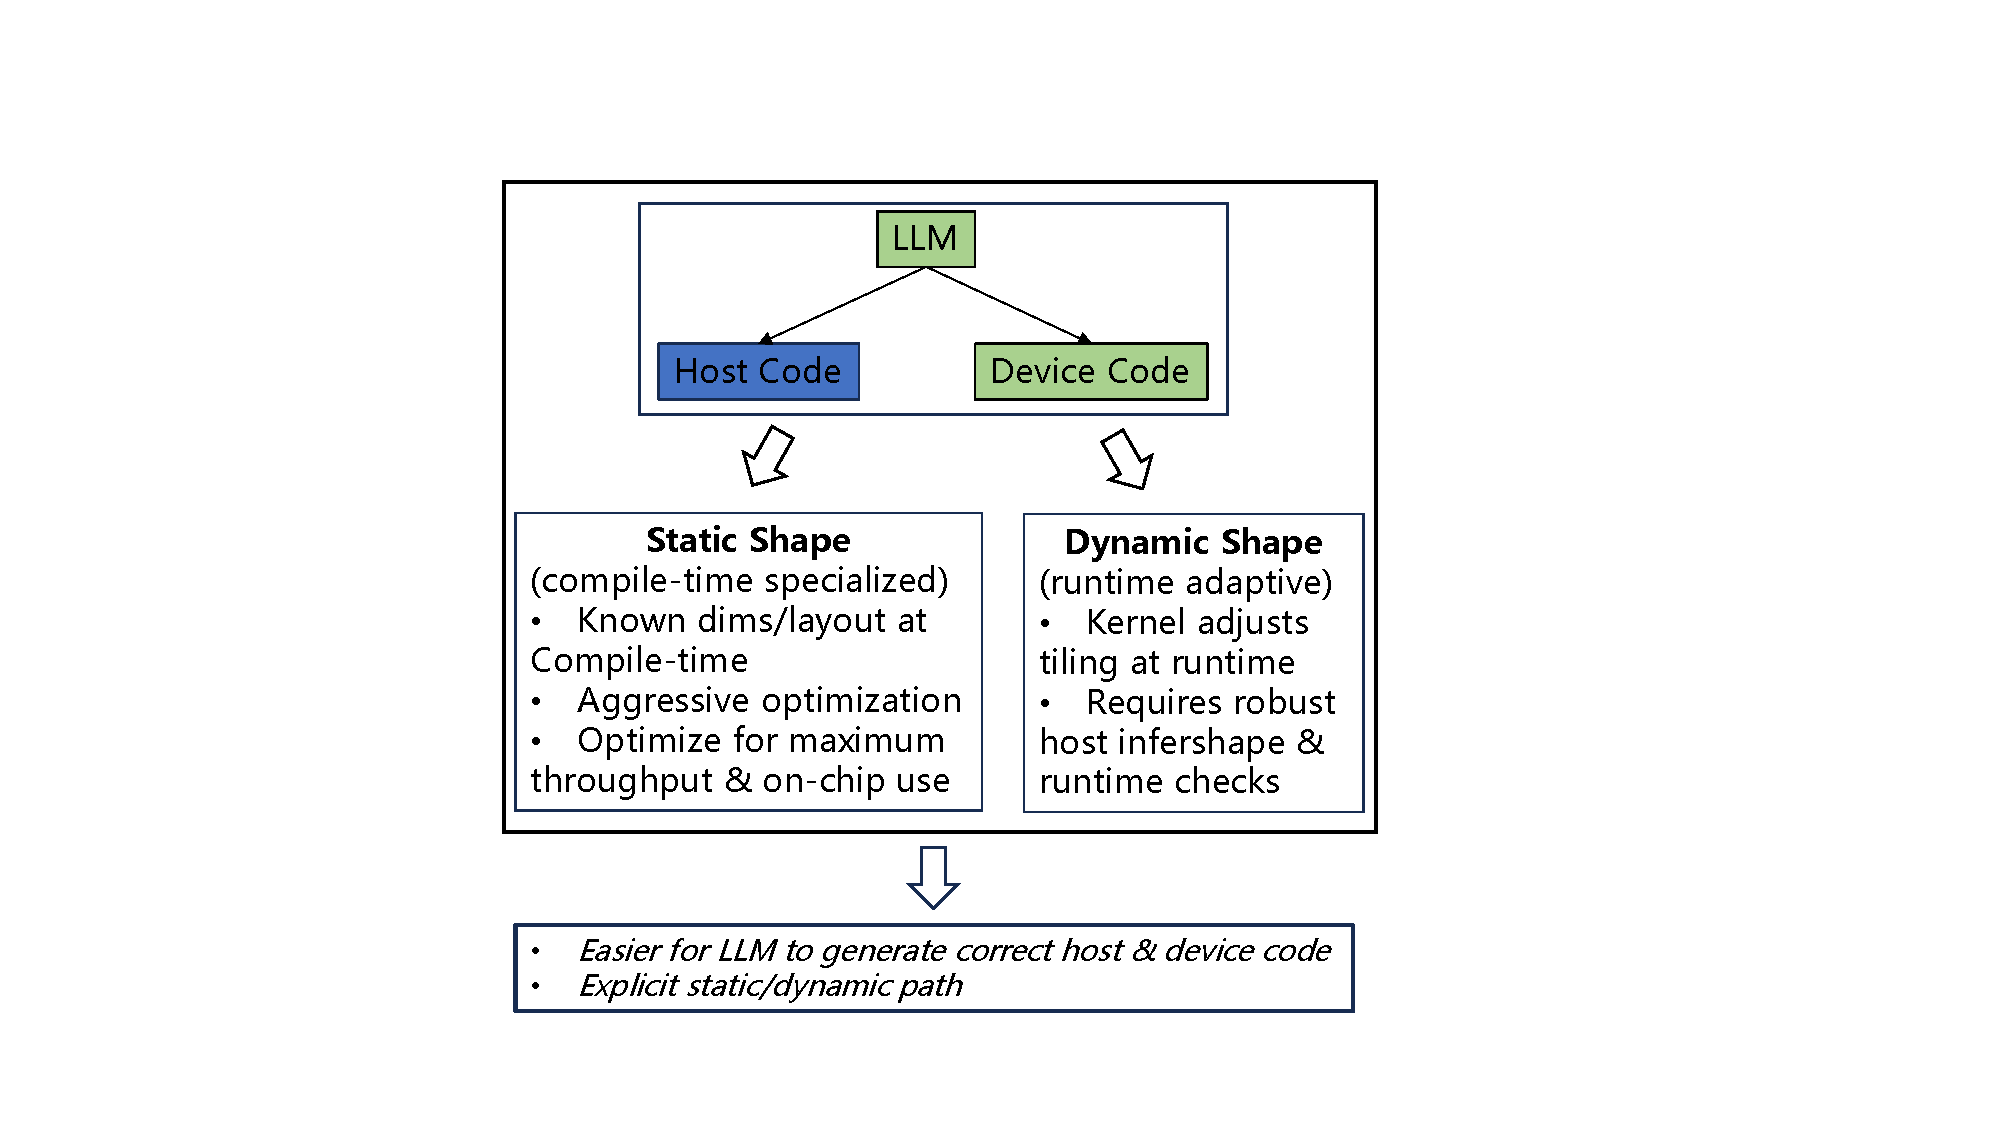
\includegraphics[
  width=\linewidth,
  trim=230pt 50pt 250pt 80pt,
  clip
]{pdfs/path.pdf}
    \vspace{-10pt}
    \caption{Dual-Path Evaluation Design.}
    \label{fig:dual_path}
    \vspace{-20pt}
\end{wrapfigure}
\paragraph{Interface Complexity.}
In addition to algorithmic difficulty, NPUKernelBench distinguishes between static-shape and dynamic-shape kernel tasks, shown in Figure~\ref{fig:dual_path}. Static-shape tasks assume compile-time known tensor dimensions and primarily evaluate specialization and optimization capability. Dynamic-shape tasks require kernels to adapt to runtime-determined dimensions, testing the model’s ability to generate robust host-side logic for shape inference, tiling computation, and control flow.




\subsection{Standardized Generation Interface}\label{sec_generate_kernel}
%The NPUKernelBench integrates a large language model (LLM) as a kernel generator to generate kernel code for the Ascend platform. Its workflow is structured around two key aspects: designing effective prompts to guide the LLM (\textit{Prompt Construction}) and specifying the precise content that the model should generate (\textit{What Content the Model Needs to Generate}). By combining carefully crafted prompts with clearly defined generation objectives, the module ensures that the LLM can understand operator requirements and produce well-structured code files.

To ensure fair and reproducible evaluation, NPUKernelBench defines a standardized generation interface that constrains both the input prompt and the structure of the generated code. This design bridges the gap between probabilistic LLM outputs and the deterministic requirements of the NPU compilation and execution pipeline.


%To ensure fair and reproducible evaluation, NPUKernelBench enforces a standardized generation interface that constrains both the input provided to the LLM and the structure of the generated output. This design bridges the gap between probabilistic text generation and the strict requirements of NPU compilation and execution.

\subsubsection{Prompt Formulation}
As illustrated in Tables~\ref{tab:prompt_ins} and \ref{tab:kernel_gen}, the prompt provided to the LLM integrates three complementary components: (1) task specification via API descriptions, (2) structural scaffolding through host and kernel code templates, and (3) role-based and formatting constraints. Together, these components provide sufficient semantic grounding and structural guidance for generating compilable Ascend C code.

%API description (\texttt{API\_Desc.md}) defines the kernel’s functionality and interface in a machine-readable markdown format. As show in Table~\ref{tab:kernel_gen}, it includes the mathematical formulation, computation process, input/output tensor specifications (names, data types, shapes, layouts, and attributes), and any constraints or hardware-specific notes. For instance, in the matrix multiplication example, the prompt explicitly describes the computational rule
%$C_{ij} = \sum_{p=1}^{k} A_{ip} B_{pj}$
%and details precision-handling strategies such as mixed-precision accumulation.
%\input{latex/tables/prompt_instructions}
%To ensure that the generated kernel code conforms to the expected software architecture and coding conventions, the framework provides pre-defined templates that serve as structural scaffolds for host and kernel implementations. These templates, located in the \texttt{tasks/.../question/} directory of each task within NPUKernelBench, specify the required code organization and interfaces. The host template defines kernel registration and tiling configuration, while the kernel template specifies the device computation entry point (e.g., \texttt{basic\_matmul\_kernel}). Table \ref{tab:kernel_gen} in Appendix show a whole template for generating Ascend kernel code.
%By leveraging these templates, the framework allows the LLM to focus on implementing computational logic rather than boilerplate, thereby enhancing generation consistency and reliability.
\textbf{Task Specification via API Description.} The core functional requirements are encapsulated in \texttt{API\_Desc.md}. As shown in Table~\ref{tab:kernel_gen}, this module translates the mathematical definition of the kernel into machine-readable specifications, detailing input/output tensor attributes (shapes, data types, layouts) and hardware constraints. For example, for a matrix multiplication kernel, the prompt explicitly formalizes the computation rule $C_{ij} = \sum_{p=1}^{k} A_{ip} B_{pj}$ and specifies precision modes, ensuring the model grounds its generation in accurate arithmetic logic.

\textbf{Structural Scaffolding via Code Templates.} To decouple algorithmic logic from boilerplate syntax, NPUKernelBench injects pre-defined code templates located in the \texttt{tasks/.../question/} directory. The prompt includes a host template (defining runtime registration and tiling interfaces) and a kernel template (specifying device-side entry points, e.g., \texttt{basic\_matmul\_kernel}). Table \ref{tab:kernel_gen} in the Appendix demonstrates a full template instance. This scaffolding forces the LLM to complete valid C++ structures rather than generating free-form text, significantly improving the compilability of the output.
\begin{wraptable}{l}{0.5\textwidth}
\vspace{-10pt}
\centering
\begin{tcolorbox}[
      sharp corners,
      colframe=reforange,
      colback=reforange!5,
      colbacktitle=reforange!15,
      coltitle=reforange,
      boxrule=0.4pt,
      title={\textbf{Instructions}},
      fonttitle=\bfseries\small,
      left=0.5pt,
      right=0.5pt,
      top=0.5pt,
      bottom=0.5pt
    ]
{\small
\begin{itemize}[leftmargin=*, itemsep=1pt, parsep=0pt, topsep=2pt]
    \item \textbf{Role:} "You are a professional Ascend kernel development engineer."
    \item \textbf{Target Language and API:} "Please use Ascend C for development."
    \item \textbf{Code Style Requirements:} "Ensure high code readability and include necessary comments."
    \item \textbf{Output Format Requirements:} "Generate separate Kernel and Host code: the Kernel defines <kernel\_name>\_kernel, and the Host declares Operator<OperatorName>Paras and implements the corresponding computation logic."
    \item \textbf{Key Information Reminder:} "Pay attention to handling the tensor data types, shapes, and layouts properly."
\end{itemize}
}
\end{tcolorbox}
\vspace{-10pt}
\captionof{table}{General instructions used in the prompt.}
\label{tab:prompt_ins}
\vspace{-10pt}
\end{wraptable}

At the beginning of a prompt, there are usually several general instructions, as illustrated in the left Table~\ref{tab:prompt_ins}. These instructions provide meta-level guidance that defines the model’s behavior, coding conventions, and output formatting. Specifically, they include explicit role prompts (e.g., adopting the perspective of a professional Ascend kernel engineer), target language and environment specifications (e.g., using Ascend C), code style requirements (e.g., ensuring readability and including necessary comments), and output format constraints (e.g., generating separate Kernel and Host code with clearly defined function and structure names). By providing sufficiently detailed instructions, the framework ensures that the LLM can follow consistent generation patterns and produce code that aligns with the target development standards.

\textbf{Role-Based Constraints.} The prompt begins with meta-instructions (Table~\ref{tab:prompt_ins}) that configure the model's persona (e.g., "Professional Ascend Kernel Development Engineer") and impose strict formatting rules. These instructions explicitly forbid conversational filler and mandate the separation of Host and Kernel code blocks. By formalizing these constraints, the framework ensures that the raw output from the LLM requires minimal post-processing before entering the compilation pipeline.

%Overall, the construction of a complete prompt follows a clear sequential process that integrates all necessary information for kernel generation. 
%First, the framework reads the task’s \texttt{api\_desc.md}, providing the model with a precise understanding of the kernel’s functionality and interface. 
%Next, the host and kernel code templates from the \texttt{question/} directory are incorporated, defining the expected structure and organization of the generated code. 
%Finally, general instructions specifying role, coding conventions, and output format are appended to guide the model’s behavior. 
%By integrating these elements in sequence, the framework ensures that the LLM receives all necessary information in a coherent and structured manner, enabling the generation of consistent and semantically correct kernel code.

Overall, the prompt formulation follows a deterministic sequence: ingesting the \texttt{api\_desc.md}, appending structural templates, and prepending constraint instructions. This creates a cohesive input context that maximizes the model's potential for generating compliant Ascend C code.

%On the input side, each prompt integrates three complementary components: (1) a formal API-based task specification, (2) structural code templates for host and kernel logic, and (3) explicit generation constraints that define coding conventions and output format. Together, these components provide sufficient context and structure while preventing unconstrained or ill-formed outputs.

\begin{comment}

The prompt provided to the LLM integrates three complementary components: (1) task specification via API descriptions, (2) structural scaffolding through host and kernel code templates, and (3) role-based and formatting constraints. Together, these components provide sufficient semantic grounding and structural guidance for generating compilable Ascend C code.

Task specifications are encoded in \texttt{API\_Desc.md}, which formalizes the mathematical definition of the kernel and specifies tensor attributes, precision modes, and hardware constraints. Structural scaffolding is provided through predefined host and kernel templates, which enforce valid C++ structure and isolate algorithmic logic from boilerplate syntax. Finally, role-based constraints define the model’s persona, coding conventions, and output format, ensuring consistency across generated samples.

\end{comment}

\subsubsection{Output Code Specification \& Dual-Path Evaluation}

NPUKernelBench enforces a strict output code specification to enable fully automated compilation and execution. Based on this specification, the framework supports a dual-path evaluation mechanism that assesses kernel generation capability under different system assumptions.

Specifically, NPUKernelBench supports two complementary evaluation paths. In the \emph{Device-Only Path}, the framework provides a fixed, pre-optimized host driver and evaluates the LLM solely on its ability to generate correct and efficient kernel-side code. This setting isolates the model’s fundamental capability in implementing core computational logic on the NPU and is particularly suitable for L1/L2 operators with minimal control flow. In contrast, the \emph{Host+Device Path} evaluates the model’s ability to generate complete, deployable operators. Under this setting, the LLM is required to produce both host-side control logic and kernel-side implementation, reflecting realistic deployment scenarios where runtime scheduling, shape inference, and dynamic memory management are essential.

\begin{comment}

In the \emph{Device-Only} path, a fixed host driver is provided and evaluation focuses exclusively on kernel-side code generation. In the \emph{Host+Device} path, the model is required to generate both host-side control logic and kernel-side implementation, reflecting realistic deployment scenarios involving shape inference, tiling computation, and runtime scheduling.

\end{comment}

%\textbf{a. Host-side code.}  This code runs on the CPU (host) and is responsible for preparing data, invoking the kernel, and processing results. The LLM is expected to:  
%\begin{itemize}
%    \item Define the parameter structure (\texttt{Operator<OperatorName>Paras}) for parsing and passing kernel attributes.  
%    \item Implement the \texttt{InferShape} function to derive output shapes from input tensors.  
%    \item Implement or invoke the Tiling function to compute kernel block information and parameters.  
%    \item Implement the logic for selecting kernel launch \texttt{BlockDim}.
%\end{itemize}

To support the Host+Device path, the output specification requires the generated code to instantiate three logically distinct but tightly coupled components within the provided templates (Table~\ref{tab:kernel_gen}). First, the host-side logic executes on the CPU and is responsible for orchestrating operator execution. This includes defining parameter structures for host–device communication, performing shape inference to derive output tensor dimensions at runtime, computing tiling parameters tailored to the target NPU architecture, and configuring kernel launch dimensions. Second, the kernel-side logic executes on the NPU AI Core and implements the parallel computation itself. The generated kernel must conform to the Ascend C programming model, correctly manage on-chip memory hierarchies, synchronize parallel execution, and employ SIMD-style computation with techniques such as double buffering to overlap data movement and computation. Finally, for operators with decoupled tiling logic, the framework expects an explicit tiling structure definition that bridges host-side tiling computation and kernel-side execution.

\begin{comment}

To support this comprehensive Host+Device path, the framework requires the LLM to instantiate three distinct logic components within the provided templates (Table~\ref{tab:kernel_gen}):

\textbf{a. Host-side Logic.} Executing on the CPU, this component manages the runtime environment. The framework requires the model to: \begin{itemize} \item Define the parameter structure (\texttt{Operator<Name>Paras}) for host-device communication. \item Implement \texttt{InferShape} logic to calculate output tensor dimensions dynamically. \item Compute Tiling parameters to optimize data block sizes for the specific NPU architecture. \item Configure the kernel launch dimensions (\texttt{BlockDim}). \end{itemize}

\textbf{b. Kernel-side Logic.} Executing on the NPU's AI Core, this component contains the parallel computational logic. The specification requires:  
\begin{itemize}
    \item Adherence to the Ascend C function signature (e.g., \texttt{extern ``C'' \_\_global\_\_ \_\_aicore\_\_ void <kernel\_name>(...)}).  
    \item Implementation of the Single Instruction Multiple Data (SIMD) logic, including double-buffering for data movement and vector/matrix computation instructions.
    \item Proper handling of synchronization barriers and memory hierarchies (Global Memory $\leftrightarrow$ Local Memory).
    \item Support different data types and shapes according to the specifications in \texttt{API\_Desc.md}.
\end{itemize}

\textbf{c. Tiling Structure Definition.}  
For complex operators requiring decoupled tiling logic, the framework expects a dedicated header definition that encapsulates the tiling data structure, ensuring it aligns with the host-side calculation.
% \begin{itemize}
%     \item Define the tiling structure or class used to organize and manage block-level computation parameters.
% \end{itemize}

\end{comment}

%In summary, we expect LLM to generate a complete Ascend operator C++ implementation—including Kernel, Host, and optionally Tiling logic, based on the semantic description in \texttt{API\_Desc.md} and the structural guidance of the code templates. The generating code must be functionally correct, syntactically compliant, and ready for compilation and execution within the framework. 
\begin{comment}

\vspace{1ex}
\noindent\textbf{Enabling Comprehensive Scenario Evaluation.}
The flexibility of this dual-path architecture and strict specification establishes NPUKernelBench as the first framework capable of comprehensively assessing kernels in two typical industrial scenarios:

\begin{enumerate}
    \item \textbf{Static Shape Optimization:} By analyzing the generated Kernel and Tiling logic, the framework evaluates the model's ability to produce extremely optimized code for fixed dimensions. Key assessment points include the design of tiling strategies, efficient management of on-chip memory (\texttt{LocalTensor}), and the optimization of computation/memory access pipelines.
    
    \item \textbf{Dynamic Shape Robustness:} Leveraging the \textbf{Host+Device Path}, the framework assesses the model's generalization ability. Since tensor shapes are unknown until runtime, the generated Host code must possess adaptive logic (e.g., dynamically calculating Tiling parameters and loop boundaries in \texttt{InferShape}). This effectively tests the robustness of the LLM-generated code in real-world, dynamic deployment environments.
\end{enumerate}

\end{comment}

This dual-path design enables NPUKernelBench to comprehensively evaluate kernel generation capability across two representative industrial scenarios, shown in Figure~\ref{fig:dual_path}. For \emph{static shape optimization}, the framework analyzes the generated kernel and tiling logic to assess whether the model can produce highly optimized code for fixed problem sizes, focusing on tiling strategy design, efficient use of on-chip memory, and compute–memory pipeline optimization. For \emph{dynamic shape robustness}, enabled by the Host+Device path, the framework evaluates the model’s ability to generalize to runtime-varying tensor shapes. In this setting, correctness and performance depend on adaptive host-side logic—such as dynamically computed tiling parameters and loop bounds—thereby testing the robustness of LLM-generated code in realistic deployment environments.


%On the output side, the framework requires the LLM to generate code that conforms to a fixed specification, enabling direct compilation and execution without manual intervention. Importantly, this specification supports two evaluation modes. In a \textit{device-only} mode, the LLM is evaluated on its ability to implement core kernel logic given a fixed host driver. In a \textit{host--device} mode, the model must generate a complete operator, including host-side control logic and kernel-side computation, reflecting realistic deployment scenarios.

By standardizing both prompt formulation and output structure, NPUKernelBench isolates model capability from prompt engineering artifacts and ensures that evaluation outcomes reflect genuine differences in kernel generation ability rather than formatting or interface inconsistencies.

\subsection{Automated Evaluation Pipeline}

NPUKernelBench is not merely a collection of test cases but a resilient, end-to-end automation framework designed to bridge the gap between model generation and rigorous hardware verification. As illustrated in Fig.~\ref{fig:framework}, the pipeline seamlessly integrates four traditionally isolated stages: \textit{Code Generation}, \textit{Compilation}, \textit{Correctness Verification}, and \textit{Performance Benchmarking}.

\begin{comment}

As illustrated in Fig.~\ref{fig:NPUKernelBench_framework}, NPUKernelBench implements a fully automated evaluation pipeline that integrates code generation, compilation, correctness verification, and performance benchmarking. The entire process is executed from a single entry point with unified configuration, enabling large-scale and reproducible evaluation.

To support high-throughput evaluation, the framework adopts a concurrent execution model with strict fault isolation. Each kernel is compiled and executed in an independent subprocess, preventing individual failures from disrupting the global pipeline. Timeout control, automatic retries, and resource cleanup further ensure robustness under long-running experiments.

\end{comment}

\subsubsection{End-to-End Architecture and Concurrency}
%To facilitate large-scale, reproducible experiments (e.g., $N=100$ samples per task), the framework adopts a "One-Click" design philosophy. Researchers can initiate the entire workflow through a single entry point (\texttt{run\_multi\_test.py}) configured via a unified definition file (\texttt{base\_config.yaml}), eliminating manual handovers between stages.

%To support the evaluation of thousands of samples across complex NPU operators, the pipeline incorporates a \textbf{Robust High-Concurrency Mechanism}:

To support large-scale and reproducible experiments (e.g., $N \geq 100$ samples per task), the framework follows a \emph{one-click} execution philosophy. The entire evaluation process is initiated from a single entry point (\texttt{run\_multi\_test.py}) and configured through a unified definition file (\texttt{base\_config.yaml}), eliminating manual intervention and reducing inconsistencies across experimental runs.

At scale, evaluating thousands of LLM-generated kernels across diverse NPU operators requires not only parallelism but also strong fault isolation. To this end, NPUKernelBench adopts a high-concurrency execution model based on Python \texttt{multiprocessing}, enabling parallel compilation and execution to maximize host CPU and NPU utilization. Each kernel evaluation is executed within a strictly isolated subprocess, ensuring that fatal errors—such as segmentation faults, illegal memory access, or NPU runtime exceptions—are contained locally and never propagate to disrupt the global pipeline.

Given the stochastic nature of LLM outputs and the complexity of hardware execution, the pipeline further incorporates native stability mechanisms to guarantee long-running robustness. Specifically, timeout control is used to proactively terminate non-terminating kernels or hardware hangs, while an automatic retry mechanism mitigates transient failures caused by network instability during API calls or temporary resource contention. In parallel, an active resource monitor enforces strict cleanup of host memory and NPU VRAM after each subprocess terminates, preventing resource leakage and ensuring consistent system behavior throughout extended batch evaluations.

Beyond execution robustness, NPUKernelBench is designed as a dedicated benchmarking suite with a structured, multi-level evaluation methodology tailored to custom NPU kernels. The framework evaluates generated operators along two primary dimensions: correctness and utilization, while adhering to three guiding principles. First, \emph{Correctness First} establishes functional validity as a prerequisite for any performance assessment. Second, \emph{Performance-Oriented Evaluation} emphasizes the effective utilization of NPU hardware resources once correctness is ensured. Third, \emph{Multi-Level Difficulty} introduces progressively more challenging tasks, enabling systematic assessment of optimization capability from basic implementations to highly tuned kernels.

These principles are realized through a fully automated evaluation pipeline comprising three tightly integrated stages: compilation evaluation, correctness evaluation, and performance evaluation. Generated kernels are first compiled to verify syntactic and build correctness, then executed on available NPU devices to validate numerical accuracy, and finally benchmarked to collect performance metrics such as execution latency and resource utilization. All stages are scheduled and executed in parallel whenever possible, with detailed logs and intermediate results recorded automatically. This design enables large-scale, objective, and reproducible evaluation of kernel generation quality with minimal human intervention.

\begin{comment}

\begin{itemize}
    \item \textbf{Parallelism \& Strict Isolation:} The framework leverages \texttt{multiprocessing} to parallelize compilation and execution, maximizing Host CPU and NPU utilization. Crucially, each evaluation task runs in a strictly isolated subprocess. This sandbox design ensures that a single kernel failure (e.g., a segmentation fault or NPU memory overflow) never propagates to crash the main pipeline.
    
    \item \textbf{Stability Assurance:} To handle the stochastic nature of LLMs and hardware interactions, the pipeline includes native \textbf{Timeout Handling} and \textbf{Auto-Retry} mechanisms. Transient failures caused by network fluctuations (during API calls) or resource contention trigger automatic retries, while infinite loops or hardware hangs are preemptively terminated to maintain overall progress.
    
    \item \textbf{Resource Recycling:} An active monitor tracks system resources, enforcing strict garbage collection of CPU memory and NPU VRAM after each subprocess terminates. This prevents resource leakage during long-running batch evaluations, ensuring consistent performance from the first sample to the last.
\end{itemize}

To comprehensively evaluate the capabilities of custom kernels on NPU, \textit{NPUKernelBench} is designed as a dedicated benchmarking suite featuring a structured and multi-level evaluation framework. Specifically, it assesses kernel implementations across two key dimensions, \textbf{correctness} and \textbf{efficiency}, while adhering to three core principles that ensure both scientific rigor and practical usability on the Ascend platform. Among them, \textit{Correctness First} underscores that functional accuracy serves as the foundation of all evaluations, \textit{Performance Goal} encourages developers to pursue maximal hardware efficiency once correctness is guaranteed, and \textit{Multi-level Difficulty} introduces progressively challenging tasks to assess optimization capability from basic to advanced levels.

Building on these principles, \textit{NPUKernelBench} employs a highly automated evaluation pipeline that ensures objectivity and reproducibility. The pipeline includes three stages: \textbf{compilation evaluation}, \textbf{correctness evaluation}, and \textbf{performance evaluation}. Each stage is executed in parallel whenever possible to improve efficiency. Generated kernels are compiled to check build correctness, tested for functional accuracy across available NPU, and subsequently benchmarked for performance metrics such as execution time and resource utilization. Throughout the process, the framework automatically manages task scheduling, logs detailed progress, and stores intermediate results, enabling large-scale, consistent, and transparent evaluation with minimal human intervention.

\end{comment}

\subsubsection{Compilation Evaluation}
In this stage, each generated kernel in Sec.~\ref{sec_generate_kernel} is first verified to ensure that it conforms to the Ascend C syntax and can be successfully compiled. To achieve this, the kernel is processed using the Ascend C compiler, and the compilation status is recorded as either success or failure. Meanwhile, detailed logs are stored in the \texttt{log/} directory of each kernel sample, which allows developers to inspect the corresponding \texttt{log\_file} in order to identify and diagnose any compilation errors. To illustrate this process, Table~\ref{tab:comp_log} presents a sample compilation log, highlighting the successful build of the \texttt{Sqrt} kernel from Level 1.

\begin{table}[H]
\vspace{-10pt}
\centering
\begin{tcolorbox}[
      sharp corners,
      colframe=refpurple,
      colback=refpurple!5,
      colbacktitle=refpurple!15,
      coltitle=refpurple,
      boxrule=0.4pt,
      title={\textbf{Compilation Log}},
      fonttitle=\bfseries\small,
      left=0.5pt,
      right=0.5pt,
      top=0.5pt,
      bottom=0.5pt
    ]
    \begin{lstlisting}[style=mystyle]
[INFO] Task lvl1_categoryMath_Sqrt_sample0 compile result:
==========================================================================================================
CompileResult:
success = True
log_file:
runs/msopgen/lvl1/Math/Sqrt/fixed_case_0/sample0/log/lvl1_categoryMath_Sqrt_sample0_compile.log
==========================================================================================================
\end{lstlisting}
\end{tcolorbox}
\captionof{table}{Compilation log of the \texttt{Sqrt} kernel using the Ascend C compiler. }
\label{tab:comp_log}
\vspace{-10pt}
\end{table}



\subsubsection{Correctness Evaluation}\label{kernelbench_correctness}

%In the correctness evaluation stage, multiple test cases are predefined for each keenel task to comprehensively cover various combinations of data types and tensor shapes. The evaluation framework then automatically compiles and executes each submitted kernel, comparing its output element-wise against the pre-generated \textit{golden reference}. A test case is considered passed only when its output satisfies the predefined accuracy tolerance. Building upon these results, the system computes the correctness score for each kernel task based on the proportion of passed test cases. This per-task score is subsequently integrated into a hierarchical scoring system that encompasses the \textbf{Task Level Score}, the \textbf{Difficulty Level Score}, and ultimately the \textbf{Total Score}.

The correctness evaluation stage assesses whether LLM-generated kernels produce numerically valid results across diverse input configurations. For each kernel task, NPUKernelBench defines a set of test cases that collectively cover relevant combinations of data types and tensor shapes. Each generated kernel is automatically compiled and executed, and correctness is determined by element-wise comparison against a pre-generated \textit{golden reference} under predefined numerical tolerances. These test outcomes form the basis of a unified and hierarchical correctness scoring scheme.

\begin{comment}

\textbf{Task-Level Score} is a unified metric that evaluates the overall correctness of a kernel across all associated test cases, serving as an indicator of both stability and robustness under diverse input conditions:
\begin{equation}
   Score_{task} = \frac{\text{Number of Passed Test Cases}}{\text{Total Number of Test Cases}} \times 100 
\end{equation}
Specifically, the task-level score directly reflects kernel correctness:
\begin{itemize}
\item A task receives a full score of \textbf{100} when all test cases pass successfully, indicating perfect correctness.
\item If only a portion of the test cases pass (e.g., a dynamic operator fails on certain input shapes), the score is proportional to the pass rate, such as \textbf{80} for 80\% accuracy.
\item If none of the test cases pass, the score drops to \textbf{0}, reflecting the principle that {correctness is prioritized over all other factors} in the evaluation process.
\end{itemize}

\end{comment}


At the task level, correctness is quantified using a single \textbf{Task-Level Score}, defined as the proportion of test cases that pass successfully:
\begin{equation}
   Score_{task} = \frac{\text{Number of Passed Test Cases}}{\text{Total Number of Test Cases}} \times 100.
\end{equation}
This abstraction intentionally treats all test cases within a task uniformly, providing a simple yet robust measure of functional validity. A kernel achieves a full score when it passes all test cases, while partial correctness is reflected by a proportionally reduced score. Kernels that fail all test cases receive a score of zero, reinforcing the principle that correctness is a strict prerequisite for any further evaluation.


\begin{comment}

This unified metric is consistently applied to all kernel tasks, which can be categorized as either \textit{static-shape} or \textit{dynamic-shape} tasks, as summarized in Table~\ref{tab:kernels}. In particular:

\begin{itemize}
\item \textbf{Static-shape tasks} correspond to a single, fixed input shape, and all test cases under such a task are dedicated to evaluating the correctness of the kernel for this specific shape.
\item \textbf{Dynamic-shape tasks} require a general-purpose kernel capable of handling multiple input shapes. Accordingly, the test cases include $M$ different shapes to comprehensively assess both the robustness and accuracy of the same kernel implementation.
\end{itemize}

\end{comment}

The same task-level metric is applied consistently to both static-shape and dynamic-shape tasks (Table~\ref{tab:kernels}). For static-shape tasks, all test cases correspond to a single fixed input configuration and jointly verify correctness for that shape. In contrast, dynamic-shape tasks require a single kernel implementation to handle multiple input shapes. As a result, multiple test cases are associated with each task, making shape generality an inherent requirement for achieving a high task-level score. Failure on any required shape directly reduces the score, naturally exposing limitations in robustness and adaptability.


%As a result, the task-level score not only measures correctness but also serves as a quantitative indicator of a dynamic operator’s generality: a kernel that fails to handle all required shapes receives a proportionally lower score, naturally reflecting its limitations in supporting multiple input configurations.

\begin{comment}

\textbf{Difficulty Level Score} for each difficulty level (L1, L2, L3) is defined as the arithmetic mean of all task scores within that level, providing a measure of overall performance at the corresponding difficulty.
\begin{equation}
   Score_{L1} = \operatorname{Average}_{i \in \text{L1 tasks}} (Score_{task_i})
\end{equation}

\end{comment}

To summarize correctness performance at higher levels of abstraction, NPUKernelBench further defines a \textbf{Difficulty-Level Score}. For each difficulty tier (L1, L2, and L3), this score is computed as the arithmetic mean of all task-level scores within that tier:
\begin{equation}
   Score_{Lk} = \operatorname{Average}_{i \in \text{Lk tasks}} (Score_{task_i}), \quad k \in \{1,2,3\}.
\end{equation}
This aggregation provides a stable estimate of correctness performance across tasks of similar complexity, mitigating variance introduced by individual operators.


\begin{comment}

\textbf{Total Score} is computed as the weighted sum of the scores for the three difficulty levels, with the weights reflecting the relative difficulty and importance of each level:

\begin{equation}
   Score_{final} = (Score_{L1} \times w_{L1}) + (Score_{L2} \times w_{L2}) + (Score_{L3} \times w_{L3})
\end{equation}

Recommended weights (configurable) are:

\[
w_{\text{L1}} = 0.2, \quad w_{\text{L2}} = 0.3, \quad w_{\text{L3}} = 0.5
\]

By assigning higher weights to more difficult levels, this scoring scheme encourages developers to tackle and solve complex tasks, thereby rewarding proficiency in challenging scenarios. Table~\ref{tab:kernel_correctness} illustrates the correctness evaluation under both default and custom criteria.

\end{comment}

Finally, an overall \textbf{Total Correctness Score} is computed as a weighted sum of the difficulty-level scores:
\begin{equation}
   Score_{final} = (Score_{L1} \times w_{L1}) + (Score_{L2} \times w_{L2}) + (Score_{L3} \times w_{L3}),
\end{equation}
where higher weights are assigned to more challenging tasks to emphasize correctness on complex operators. By default, the framework uses $w_{\text{L1}} = 0.2$, $w_{\text{L2}} = 0.3$, and $w_{\text{L3}} = 0.5$. This design encourages models to prioritize correctness on difficult tasks and serves as a gating signal for subsequent performance evaluation. Scoring criteria for kernel evaluation is given in Table~\ref{tab:level_correctness}. Representative evaluation criteria under both default and customized settings are also given in Table~\ref{tab:kernel_correctness}.


\begin{table}[t]
\centering
\caption{Scoring criteria for kernel evaluation.}
\resizebox{1\linewidth}{!}{
\begin{tabular}{lll}
\hline
\textbf{Scoring Item} & \textbf{Formula} & \textbf{Core Idea} \\
\hline
Task Score & $ \text{Score}_{\text{task}} = \frac{\text{Number of Passed Test Cases}}{\text{Total Number of Test Cases}} \times 100 $ & Measures correctness and serves as the foundation of the overall score. \\
Level Score & $ \text{Average}(\text{Score}_{\text{task}_j}) $ & Reflects the overall performance at a given difficulty level. \\
Total Score & $ \sum (\text{Score}_{\text{level}} \times w_{\text{level}}) $ & Weighted sum incentivizing completion of higher-difficulty tasks. \\
\hline
\end{tabular}}
\label{tab:level_correctness}
\end{table}

%\input{latex/tables/correctness_eva}

\begin{comment}

\subsubsection{Performance Evaluation}
The primary metric for performance evaluation is the execution latency of a kernel on the NPU. To ensure fairness and stability, each test case undergoes several warmup iterations, followed by $N$ consecutive runs, and the average execution time is taken as the final performance measurement for that test case.

Performance is assessed relative to an objective \textit{performance ceiling} benchmark, denoted as $T_{\text{roofline}}$. This benchmark represents the theoretically minimal execution time achievable for the given kernel and tensor shape on the current hardware. In practice, $T_{\text{roofline}}$ is typically approximated using highly optimized implementations from official NPU vendor libraries (e.g., \texttt{aclnn}), which serve as a reliable reference for comparison.

\end{comment}

\subsubsection{Performance Evaluation}

The performance evaluation stage measures the execution efficiency of LLM-generated kernels on the target NPU. The primary metric is kernel execution latency. To ensure stability and comparability, each test case is executed with a fixed number of warm-up iterations to mitigate cold-start effects, followed by $N$ consecutive runs. The average execution time across these runs is reported as the performance measurement for the test case.

Rather than reporting absolute latency alone, NPUKernelBench evaluates performance relative to a hardware-aware reference upper bound, denoted as $T_{\text{ref}}$. This reference time reflects the execution latency achieved by highly optimized vendor-provided kernels for the same operator and tensor configuration on the target NPU. $T_{\text{ref}}$ does not represent a strict theoretical lower bound on execution time. Instead, it serves as a strong and practically attainable performance reference, instantiated using mature and well-engineered implementations from official NPU libraries (e.g., \texttt{aclnn}). While such vendor kernels may not always achieve the absolute hardware limits, they provide a stable, reproducible, and hardware-aware baseline that reflects current best engineering practices.

By normalizing kernel latency against this reference, the evaluation emphasizes how effectively a generated kernel approaches the performance level of optimized production kernels, rather than relying on raw execution time alone. This relative formulation mitigates sensitivity to operator-specific scale, tensor shapes, and hardware characteristics, enabling fair comparison across heterogeneous workloads. As in the correctness evaluation, performance is measured only for kernels that pass functional validation, ensuring that efficiency is assessed exclusively for correct implementations.

\subsection{Optimization-Ready Fine-Grained Logging}
\label{sec:logging_system}

The logging system of NPUKernelBench is designed not merely for passive record-keeping, but as a feedback mechanism that bridges evaluation and model optimization. By systematically capturing detailed execution traces throughout the evaluation pipeline, the framework provides fine-grained, actionable signals that support iterative improvement of LLM-based code generation models.

At each stage of the pipeline, including code generation, compilation, and correctness verification, NPUKernelBench produces structured and stage-aware logs. Rather than reporting only coarse-grained outcomes (e.g., a binary build failure), the framework records precise diagnostic information such as compiler error codes, line numbers, and mismatch details. These logs are stored in a structured format (e.g., \texttt{compile.log}), ensuring that every failure mode is traceable, reproducible, and amenable to downstream analysis.

This design transforms evaluation outputs from sparse scalar signals into rich feedback representations. Instead of reducing kernel quality to a single pass/fail outcome, the logging system exposes intermediate failure modes and partial successes, enabling more informative supervision. Such feedback can directly support manual prompt refinement as well as automated optimization pipelines, including supervised fine-tuning (SFT), where structured error patterns can be leveraged as learning signals.

Beyond supervised settings, the fine-grained logging mechanism further enables reinforcement learning based optimization. By decomposing kernel generation into a sequence of verifiable milestones, such as syntactic validity, successful compilation, numerical correctness, and performance attainment, the framework can provide dense and interpretable reward signals. These signals can be naturally mapped to reward shaping strategies, allowing incremental credit assignment during training. As a result, NPUKernelBench extends beyond a static benchmarking suite and can function as an evaluation-driven training environment, supporting the development of self-improving kernel generation agents.

\begin{comment}

\begin{itemize}
    \item \textbf{Multi-Stage, Structured Logs:} 
    The framework generates detailed and structured logs at every stage of the pipeline (\textit{code\_gen}, \textit{compile}, \textit{precision}). Unlike traditional benchmarks that may only report a binary "Build Failed" status, our system captures specific compiler diagnostics (e.g., error codes, line numbers, and mismatch details) in the \texttt{compile.log}. This ensures that every failure is traceable and actionable.

    \item \textbf{From Scalar Scores to Rich Feedback Signals:} 
    This fine-grained logging transforms the evaluation result from a \textit{sparse scalar metric} (Pass/Fail) into a \textbf{Rich Feedback Signal}. This transformation is critical for enabling model optimization, providing clear debugging evidence that can guide both manual Prompt Engineering and automated Supervised Fine-Tuning (SFT).

    \item \textbf{Reward Source for Reinforcement Learning (RL):} 
    Crucially, these structured logs serve as a direct source for \textbf{Reward Shaping} in Reinforcement Learning workflows. By decomposing the kernel generation task into verifiable milestones, the framework can provide dense feedback signals—for example, assigning incremental rewards for successful code parsing (+0.1), successful compilation (+0.5), functional correctness (+1.0), and performance targets (+2.0). This capability elevates NPUKernelBench from a static benchmarking suite to a potential \textbf{Reinforcement Learning Training Environment}, facilitating the development of self-improving coding agents in the future.
\end{itemize}

\end{comment}

% \input{latex/tables/template}
\section{Experiments and Results}
\label{experiments}

  %测试的benchmark，使用什么样的LLM大模型，强化学习的模型，
%关于数据部分的模型，做SFT和RL的模型，不同系列的开源模型，同一模型的不同scale模型。做SFT的配置，强化学习的算法等配置
% 模型角度：
% 1. 语料库构造使用的模型
% 2. SFT和RL的模型
% 3. 消融实验的模型：不同系列的开源模型，同一模型的不同scale模型
% 实验配置角度
% 4. SFT 配置 
% 5. RL 配置 （不同的数据组合方式）
\subsection{Experimental Setups}

\begin{comment}

\textbf{Models.}
As summarized in Table~\ref{tab:models_training}, we employ different large language models at each stage according to their respective roles. 
For dataset construction, {DeepSeek-R1}~\cite{abs250112948} is used for document-based data generation and single-file Chain-of-Thought (CoT) construction (Secs.~\ref{document_dataset} and~\ref{single_file}). 
To support project-level CoT construction that requires reasoning over complete kernel projects with multiple mutually referenced source files, we adopt {Gemini 2.5 Pro}~\cite{google_gemini_2_5_pro} (Sec.~\ref{project_file}), which owing to its stronger support for multi-file code understanding and cross-file dependency reasoning. 
Within the data flywheel in SFT (Secs.~\ref{sft_api_correction} and~\ref{sft_kernel_correction}), {DeepSeek-Reasoner} is further leveraged to iteratively refine and correct the generated reasoning chains.

\end{comment}

\textbf{Models.}
As summarized in Table~\ref{tab:models_training}, we employ different large language models at distinct stages of the pipeline according to their functional roles. For dataset construction and document-level reasoning, we adopt DeepSeek-R1~\cite{abs250112948}, which is used to generate document-based data and single-file Chain-of-Thought (Secs.~\ref{document_dataset} and~\ref{kernel_dataset}). For project-level reasoning that requires understanding multi-file kernel implementations with cross-file dependencies, we employ Gemini~2.5~Pro~\cite{google_gemini_2_5_pro}, leveraging its stronger support for long-context and multi-file code reasoning (Sec.~\ref{kernel_dataset}). Within the supervised fine-tuning (SFT) data, DeepSeek-Reasoner is further used to iteratively refine and correct reasoning traces (Secs.~\ref{sft_api_correction} and~\ref{sft_kernel_correction}).

%For model training, we adopt \textbf{Qwen3-32B}~\cite{qwen3technicalreport} as the backbone model for supervised fine-tuning (SFT) and reinforcement learning (RL). 
%To study the effect of model scale and architecture, we additionally conduct SFT on multiple Qwen variants, including Qwen3-1.7B, 4B, 8B, 14B, and 32B, as well as the code-specialized Qwen3-Coder-30B-A3B-Instruct.

% \noindent\textbf{Training} 
% % SFT 
% % RL 
% To effectively inject kernel-specific knowledge into the LLM, we adopt a two-stage training strategy. 
% The first stage performs SFT on the AscendC dataset constructed as described in Sec.~\ref{data_construct}, which consists of three categories: AscendC document data, AscendC kernel data, and general reasoning chains. 
% To evaluate the contribution of each category, we conduct ablation studies by removing one component at a time. 
% We also assess the impact of data scale by performing SFT with 25\%, 50\%, and 75\% of the dataset.
% The second stage is reinforcement learning (RL), we adopt Direct Preference Optimization~(DPO) \cite{RafailovSMMEF23} with a learning rate of $1\times10^{-6}$, cosine learning rate decay, and a warm-up ratio of 0.1. The global batch size is set to 64, the training runs for 150 iterations, and the DPO loss uses a sigmoid formulation with $\beta=0.1$. We also analysis different positive/negative pairs for this training preference dataset.
% We further analyze the impact of different positive and negative sample selection strategies in constructing the preference dataset Sec. \ref{reinforcement_learning} for reinforcement learning.

\begin{comment}

\noindent\textbf{Training.}
We adopt a two-stage training strategy consisting of supervised fine-tuning~(SFT) followed by reinforcement learning~(RL). 
In the first stage, SFT is performed using {Qwen3-32B}~\cite{qwen3technicalreport} as the backbone model. 
To analyze the effect of model scale and architecture, we additionally conduct SFT on multiple Qwen variants, including Qwen3-1.7B, 4B, 8B, 14B, and 32B, as well as the code-specialized Qwen3-Coder-30B-A3B-Instruct. 
All SFT experiments are conducted under a unified training setup, with comparisons between full fine-tuning and LoRA-based tuning following the configurations summarized in Table~\ref{tab:models_training}.
In the second stage, RL is conducted using {Direct Preference Optimization} (DPO)~\cite{RafailovSMMEF23} under a fixed training configuration. 
Specifically, we use a learning rate of $1\times10^{-6}$ with cosine decay and a warm-up ratio of 0.1, a global batch size of 64, and train for 150 iterations. 
We further analyze the impact of different positive and negative sample selection strategies in constructing the preference dataset, as detailed in Sec.~\ref{reinforcement_learning}.

\end{comment}

\textbf{Training.}
We adopt a two-stage training strategy consisting of supervised fine-tuning followed by reinforcement learning. In the SFT stage, Qwen3-32B~\cite{qwen3technicalreport} serves as the primary backbone model. To analyze the impact of model scale and architecture, we additionally conduct SFT on multiple Qwen variants ranging from 1.7B to 32B parameters, as well as the code-specialized Qwen3-Coder-30B-A3B-Instruct. All SFT experiments share a unified training configuration, with both full fine-tuning and LoRA-based tuning evaluated under controlled settings (Table~\ref{tab:models_training}). In the second stage, reinforcement learning is performed using Direct Preference Optimization (DPO)~\cite{RafailovSMMEF23}, with detailed configurations and ablation studies reported in Sec.~\ref{reinforcement_learning}.

\begin{table}[t]
\centering
\caption{Overview of models and configurations used for dataset construction and two-stage training.}
\label{tab:models_training}
\resizebox{0.9\linewidth}{!}{
\begin{tabular}{p{3.7cm} p{3.9cm} p{3.9cm} p{5.5cm}}
\toprule
\textbf{Stage} & \textbf{Model / Method} & \textbf{Role} & \textbf{Description} \\
\midrule

\multirow{9}{*}{Dataset Construction} %9代表description有9个物理行
& DeepSeek-R1
& Document \& Single-file CoT 
& Document-based data generation and single-file Chain-of-Thought construction \\

& Gemini 2.5 Pro
& Project-level CoT 
& Reasoning over complete kernel projects with multiple mutually referenced source files \\

& DeepSeek-Reasoner 
& Data Flywheel Refinement
& Iterative correction and refinement of generated reasoning chains within the data flywheel \\
\midrule

\multirow{10}{*}{Supervised Fine-tuning}  %10代表description列有10个物理行
& Qwen3-32B
& Backbone Model 
& Backbone model for supervised fine-tuning \\

& Qwen3-1.7B / 4B / 8B / 14B / 32B / Coder-30B-A3B-Instruct 
& Scaling Study 
& Supervised fine-tuning across different model scales and architectures \\

& Training Configuration 
& Full FT / LoRA 
& Learning rate $1.25\times10^{-6}$ (Full FT) vs. $1.25\times10^{-5}$ (LoRA), cosine decay, warm-up ratio 0.01, micro/global batch size 1/128, weight decay $1\times10^{-1}$, gradient clipping 1.0. \\

\midrule

\multirow{7}{*}{Reinforcement Learning}  %7代表description列有7个物理行
& DPO
& Optimization Objective 
& Direct Preference Optimization with $\beta=0.1$ \\

& Training Configuration 
& Hyperparameters 
& Learning rate $1\times10^{-6}$, cosine decay, warm-up ratio 0.1, global batch size 64, 150 training iterations \\

& Preference Construction 
& Ablation Analysis 
& Analysis of different positive and negative sample selection strategies \\
\bottomrule
\end{tabular}}
\end{table}


\subsection{NPUKernelBench and Evaluation Metrics} % 测试的算子介绍，评价指标编译和精度

\begin{comment}

Our evaluation is conducted on \textbf{NPUKernelBench}, as introduced in Sec.~\ref{NPUKernelBench}. 
It consists of 158 representative CANN kernels organized into three levels of computational complexity, each accompanied by a reference Python implementation with standardized input/output specifications for automated evaluation.
For each kernel, we generate AscendC code using the evaluated LLM and subsequently compile and execute the generated kernels on the target NPU platform. To assess the robustness and scalability of the generated kernels, we evaluate each task under \textbf{multiple input data sizes}, as summarized in Table xxx. This setting allows us to examine the model's generalization ability across varying workload intensities and input scales.
% \paragraph{Evaluation Metrics.}
We adopt two complementary metrics to comprehensively evaluate the quality of generated kernels:

\begin{itemize}
    \item \textbf{Compilation Rate.}  
    This metric measures whether a generated AscendC kernel can be successfully compiled by the CANN toolchain without errors. 
    A kernel is considered \emph{successfully compiled} only if it passes the full compilation process, reflecting the model's ability to generate valid and API-compliant kernel code.

    \item \textbf{Execution Rate.} 
    For kernels that compile successfully, Execution Rate is evaluated by comparing their outputs with the reference Python implementations under a predefined numerical tolerance. We additionally report correctness for different kernel complexity levels, as described in Sec.~\ref{kernelbench_correctness}.

    \item \textbf{Performance Speedup.}  This metric evaluates the runtime efficiency of generated kernels by comparing their average execution time with expert-implemented kernels. For each kernel, we compute the \emph{Speedup} as $\text{Speedup} = T_{\text{expert}} / T_{\text{gen}}$, where $T_{\text{expert}}$ and $T_{\text{gen}}$ denote the average execution time of expert-implemented and generated kernels, respectively; values greater than $1.0$ indicate performance improvement, while values below $1.0$ imply a slowdown.

\end{itemize}

\end{comment}

All evaluations are conducted on NPUKernelBench (Sec.~\ref{NPUKernelBench}), which contains 158 representative kernels spanning three levels of computational complexity.
Each kernel is accompanied by a reference implementation with standardized input and output specifications, enabling automated correctness verification.

For each task, we generate kernel code using the evaluated LLM and execute the compiled kernels on the target NPU platform. To assess robustness and scalability, each kernel is evaluated under multiple input sizes, allowing us to examine generalization behavior across varying workload intensities.

We evaluate generated kernels along three complementary dimensions. First, the \emph{Compilation Rate} measures whether a kernel can be successfully compiled, reflecting syntactic validity and API compliance; this metric is reported as pass@$k$, indicating the fraction of tasks for which at least one of the top-$k$ generated candidates compiles successfully. Second, the \emph{Execution Rate} assesses functional correctness by comparing kernel outputs against reference implementations under predefined numerical tolerances (Sec.~\ref{kernelbench_correctness}), and is likewise measured under the pass@$k$ protocol. Finally, \emph{Performance Speedup} evaluates runtime efficiency by normalizing kernel latency against expert-implemented baselines, with values greater than one indicating performance improvements.


\subsection{Main Results} %实验结果比较，未经sft的，sft，强化学习的

We compare kernel generation performance across different training stages, including the base models, supervised fine-tuning, and reinforcement learning. Overall, performance improves consistently as training progresses, with increasingly robust behavior observed on more challenging kernels. Quantitative results under different sampling budgets are summarized in Table~\ref{tab:pass_k_results_speed} and analyzed in detail below.

% \begin{table}[t]
%     \centering
%     \small
%     \renewcommand{\arraystretch}{1.1} % 稍微调整行高
    
%     % 总标题
%     \caption{Evaluation results of kernel generation on NPUKernelBench across different sampling budgets ($k$). We report Compile Rate (CR), Execution Success Rate (ESR), and Speedup for Pass@1, Pass@10, and Pass@100.}
%     \label{tab:pass_k_results}

%     % --- 子表 (a): Pass@1 ---
%     \begin{subtable}{1\linewidth}
%         \centering
%         \caption{Results for \textbf{Pass@1}}
%         \begin{tabular}{l cc c c}
%             \toprule
%             \textbf{Model} & \textbf{Level} & \textbf{Compile Rate (\%)} & \textbf{Exec. Rate (\%)} & \textbf{Speedup ($\times$)} \\
%             \midrule
%             \multirow{2}{*}{QWen3-32B}      & Level 1    & 38.08 & 17.39 & 0.85 \\
%             & Level 2    & 0.0 & 0.0 &  - \\ 
%             & Mean       & 45.72 & 11.59 & - \\ 

%             \multirow{2}{*}{QWen3-32B + SFT}  & Level 1       & 60.5 & 28.1 & 0.95 \\
%             & Level 2    & 52.4 & 21.5 & 0.85 \\ 
%             & Mean       & 52.4 & 21.5 & 0.85 \\ 
%             \multirow{2}{*}{QWen3-32B + SFT + RL}   & Level 1      & 60.5 & 28.1 & 0.95 \\
%             & Level 2    & 52.4 & 21.5 & 0.85 \\ 
%             & Mean       & 52.4 & 21.5 & 0.85 \\ 
%             \bottomrule
%         \end{tabular}
%         \label{subtab:pass1}
%     \end{subtable}
    
%     \bigskip % 添加垂直间距

%     % --- 子表 (b): Pass@10 ---
%     \begin{subtable}{1\linewidth}
%         \centering
%         \caption{Results for \textbf{Pass@10}}
%         \begin{tabular}{l cc c c}
%             \toprule
%             \textbf{Model} & \textbf{Level} & \textbf{Compile Rate (\%)} & \textbf{Exec. Rate (\%)} & \textbf{Speedup ($\times$)} \\
%             \midrule
%              \multirow{2}{*}{QWen3-32B}      & Level 1    & 52.4 & 21.5 & 0.85 \\
%             & Level 2    & 52.4 & 21.5 & 0.85 \\ 
%             & Mean       & 52.4 & 21.5 & 0.85 \\ 
%             \multirow{2}{*}{QWen3-32B + SFT}  & Level 1       & 60.5 & 28.1 & 0.95 \\
%             & Level 2    & 52.4 & 21.5 & 0.85 \\ 
%             & Mean       & 52.4 & 21.5 & 0.85 \\ 
%             \multirow{2}{*}{QWen3-32B + SFT + RL}   & Level 1      & 60.5 & 28.1 & 0.95 \\
%             & Level 2    & 52.4 & 21.5 & 0.85 \\ 
%             & Mean       & 52.4 & 21.5 & 0.85 \\ 
%             \bottomrule
%         \end{tabular}
%         \label{subtab:pass10}
%     \end{subtable}

%     \bigskip % 添加垂直间距

%     % --- 子表 (c): Pass@100 ---
%     \begin{subtable}{1\linewidth}
%         \centering
%         \caption{Results for \textbf{Pass@100}}
%         \begin{tabular}{l cc c c}
%             \toprule
%             \textbf{Model} & \textbf{Level} & \textbf{Compile Rate (\%)} & \textbf{Exec. Rate (\%)} & \textbf{Speedup ($\times$)} \\
%             \midrule
%              \multirow{2}{*}{QWen3-32B}      & Level 1    & 52.4 & 21.5 & 0.85 \\
%             & Level 2    & 52.4 & 21.5 & 0.85 \\ 
%             & Mean       & 52.4 & 21.5 & 0.85 \\ 
%             \multirow{2}{*}{QWen3-32B + SFT}  & Level 1       & 60.5 & 28.1 & 0.95 \\
%             & Level 2    & 52.4 & 21.5 & 0.85 \\ 
%             & Mean       & 52.4 & 21.5 & 0.85 \\ 
%             \multirow{2}{*}{QWen3-32B + SFT + RL}   & Level 1      & 60.5 & 28.1 & 0.95 \\
%             & Level 2    & 52.4 & 21.5 & 0.85 \\ 
%             & Mean       & 52.4 & 21.5 & 0.85 \\ 
%             \bottomrule
%         \end{tabular}
%         \label{subtab:pass100}
%     \end{subtable}
% \end{table}
\begin{table}[t]
\centering
\small
\renewcommand{\arraystretch}{1.1}
\caption{Evaluation results of kernel generation on NPUKernelBench across different sampling budgets ($k$). We report Compilation Rate (CR), Execution Rate (ER), and overall Speedup for generated kernels.}
\label{tab:pass_k_results_speed}
\resizebox{1\linewidth}{!}{
\begin{tabular}{l c cc cc cc c}
\toprule
\multirow{2}{*}{\textbf{Model}} & \multirow{2}{*}{\textbf{Level}} & \multicolumn{2}{c}{\textbf{Pass@1}} & \multicolumn{2}{c}{\textbf{Pass@10}} & \multicolumn{2}{c}{\textbf{Pass@100}} & \multirow{2}{*}{\textbf{Speedup ($\times$)}} \\
\cmidrule(r){3-4} \cmidrule(r){5-6} \cmidrule(r){7-8}
 & & CR (\%) & ER (\%) & CR (\%) & ER (\%) & CR (\%) & ER (\%) &  \\
\midrule
\multirow{4}{*}{Qwen3-32B} & Level 1 & 38.08 & 17.39 &71.62  &48.84  &75.00  &66.67  & 0.60 \\
 & Level 2 & 0.0 & 0.0 & 0.0 & 0.0 & 0.0 & 0.0 & 0.0 \\
 & Level 3 & 1.83 & 0.0 & 15.43 & 0.0 & 50.00 & 0.0 & 0.0 \\
 \rowcolor{bggreen}
 & Mean & 25.59 &11.59  & 49.46 & 32.56 & 55.56 & 44.44 & 0.60 \\
\midrule
\multirow{4}{*}{Qwen3-32B + SFT} & Level 1 &84.83  &38.28  &99.97  &86.82  &100  &94.44  & 0.56 \\
 & Level 2 &60.5 &8  &96.54  &40.48  &100 &75  & 1.50 \\
 & Level 3 &17 &0.17  &63.75  &1.67  &100 &16.67  & 0.00 \\
 \rowcolor{bggreen}
 & Mean &\textbf{71.89}  &27.31  &\textbf{95.18}  &67.06 &\textbf{100} & 81.48 &  0.75 \\
\midrule
\multirow{4}{*}{Qwen3-32B + SFT + RL} & Level 1 &82.17 &43.28 &99.92 &93.89 &100 &100 & 0.61 \\
 & Level 2 &62.75 &14.25 &95.49 &64.28 &100 &91.67 & 1.86 \\
 & Level 3 &14.67 &0.17  &61.12  &1.67  &100 &16.67  & 0.00 \\
 \rowcolor{bggreen}
 & Mean &70.35 &\textbf{32.04} &94.62 &\textbf{77.06} &\textbf{100} &\textbf{88.89} & 0.87 \\

\bottomrule
\end{tabular}}
\end{table}



\begin{figure*}
    \centering
    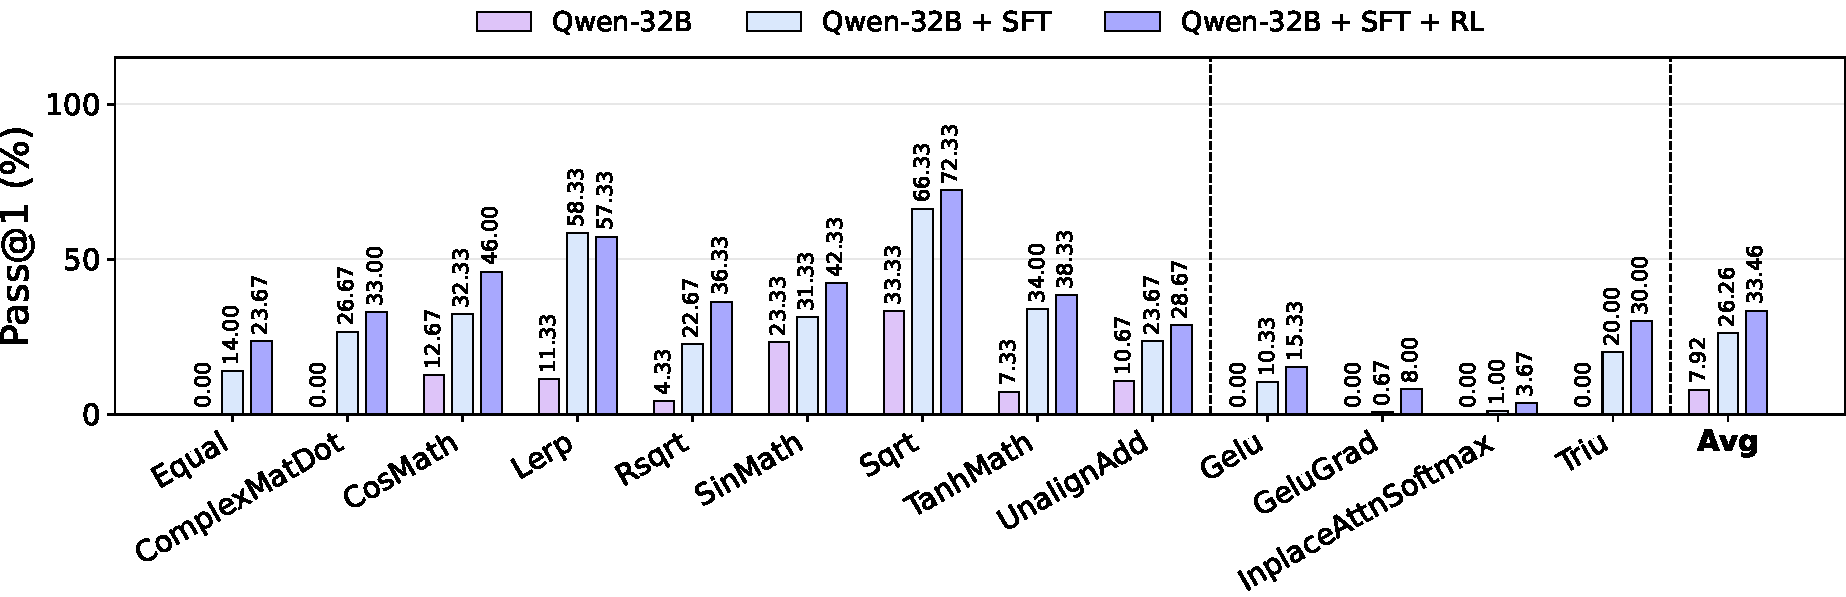
\includegraphics[width=0.98\linewidth]{pdfs/level1_level2_Avg_pass1.pdf}
    %\caption{Kernel-wise Pass@1 performance comparison of selected operators across training stages. This bar chart visualizes the accuracy of chosen kernels from Qwen-32B across Base, SFT, and RL stages. While all models show improved performance, RL particularly enhances accuracy for complex kernels, allowing for a comparative analysis of their effectiveness at each stage.}
    \caption{Pass@1 results for representative kernels across training stages.}
    \label{fig:Specific_kernel_acc}
\end{figure*}

\subsubsection{Compilation and Execution}

\begin{comment}

Table~\ref{tab:pass_k_results_speed} reports the evaluation results of kernel generation on NPUKernelBench under different sampling budgets ($k$) and difficulty levels. We observe a clear correlation between kernel difficulty and generation performance. For the base QWen3-32B model, Level 1 kernels achieve moderate Compile Rate (CR) and Execution Success Rate (ER), while Level 2 kernels are largely unsolved and Level 3 kernels show very low ER despite some improvements in CR at higher $k$. Incorporating supervised fine-tuning (SFT) substantially boosts both CR and ER across all levels, especially for Level 1 and Level 2 kernels, indicating that SFT helps the model better capture task-specific patterns. Further enhancement with reinforcement learning (RL) yields additional gains in ER, particularly for higher difficulty levels, suggesting that RL effectively guides the model toward more executable kernels. Overall, the mean performance demonstrates that hierarchical training strategies (SFT + RL) significantly improve kernel generation quality and robustness across varying kernel difficulty levels, while also achieving notable speedup in execution.

\end{comment}

Table~\ref{tab:pass_k_results_speed} summarizes kernel generation performance on NPUKernelBench across different sampling budgets ($k$) and difficulty levels.
A clear performance gap emerges as kernel complexity increases.
For the base Qwen3-32B model, Level~1 kernels achieve moderate compilation rates (CR) and execution success rates (ER), whereas Level~2 kernels remain largely unsolved.
For Level~3 kernels, although higher $k$ improves CR to some extent, ER remains consistently low, indicating that successful compilation alone does not guarantee correct execution for complex kernels.

Figure~\ref{fig:Specific_kernel_acc} presents the Pass@1 accuracy of Qwen-32B on a set of representative kernels across three training stages: the base model, supervised fine-tuning (SFT), and SFT followed by reinforcement learning (RL).
The base model exhibits limited kernel synthesis capability, achieving an average Pass@1 of only 7.92\%, which reflects the difficulty of directly transferring general-purpose code generation ability to low-level NPU kernel programming.

Supervised fine-tuning leads to a substantial improvement, increasing the average Pass@1 to 26.26\%.
This gain indicates that SFT effectively aligns the model with the structural and syntactic requirements of kernel generation, enabling it to produce compilable and partially correct implementations.
In particular, SFT equips the model with essential building blocks such as API usage patterns, memory object initialization, and canonical computation templates, which are prerequisites for valid kernel synthesis.

Building upon this foundation, reinforcement learning further improves the average Pass@1 accuracy to 33.46\%.
Unlike SFT, which primarily addresses coarse-grained correctness, RL provides execution-based preference signals that encourage the model to distinguish between multiple valid but semantically different implementations.
The resulting improvements are especially pronounced for complex kernels, where subtle errors in memory staging, accumulation order, or synchronization often determine execution success.

Overall, the progressive performance gains across training stages highlight the complementary roles of SFT and RL.
SFT establishes baseline kernel generation competence by enforcing hard compilation and correctness constraints, while RL refines fine-grained execution logic beyond syntactic validity.
This staged alignment strategy proves crucial for improving first-attempt accuracy on challenging NPU kernels, where even minor implementation errors can lead to execution failure.


\subsubsection{Performance Speedup}

Beyond functional correctness, Table~\ref{tab:pass_k_results_speed} further evaluates the runtime efficiency of the generated kernels on real Ascend NPU hardware. 
The base model exhibits limited optimization capability, achieving only a $0.60\times$ speedup on Level~1 tasks and failing entirely on Level~2 and Level~3 kernels. 
This behavior indicates that general-purpose code generation lacks the ability to reason about hardware-specific parallelism and memory hierarchies.

In contrast, the proposed training pipeline yields substantial and systematic performance improvements. 
After supervised fine-tuning, the model not only recovers executable kernels but also learns performance-oriented implementation strategies. 
In particular, SFT achieves a $1.50\times$ speedup on Level~2 tasks, surpassing expert-written baselines. 
This result suggests that exposure to kernel-centric reasoning patterns enables the model to internalize optimized tiling, memory reuse, and operator fusion strategies that are difficult to infer from generic code corpora alone.

Reinforcement learning further refines these implementations by incorporating execution-based preference signals. 
On Level~2 kernels, RL improves the average speedup to $1.86\times$, while maintaining stable performance on Level~1 tasks ($0.61\times$). 
These gains primarily stem from fine-grained adjustments to memory access ordering, synchronization placement, and accumulation structure, rather than large-scale structural changes introduced during SFT.

Performance improvements are most pronounced on Level~2 tasks, where structured computation and localized data dependencies provide sufficient flexibility for optimization while remaining amenable to model-driven reasoning. 
In contrast, Level~1 kernels offer limited optimization space, and Level~3 kernels remain challenging due to global dependencies and complex control flow. 
Overall, these results indicate that the proposed SFT+RL pipeline enables the model to generate not only syntactically valid kernel code, but also hardware-efficient parallelization patterns, achieving expert-level and even expert-surpassing performance on a broad class of practical NPU operators.


\subsection{Ablation Analysis of Supervised Fine-tuning}

\subsubsection{Model Scale Sensitivity} 
% 不同规模 Qwen 模型的 SFT 性能对比
\begin{figure}
    \centering
    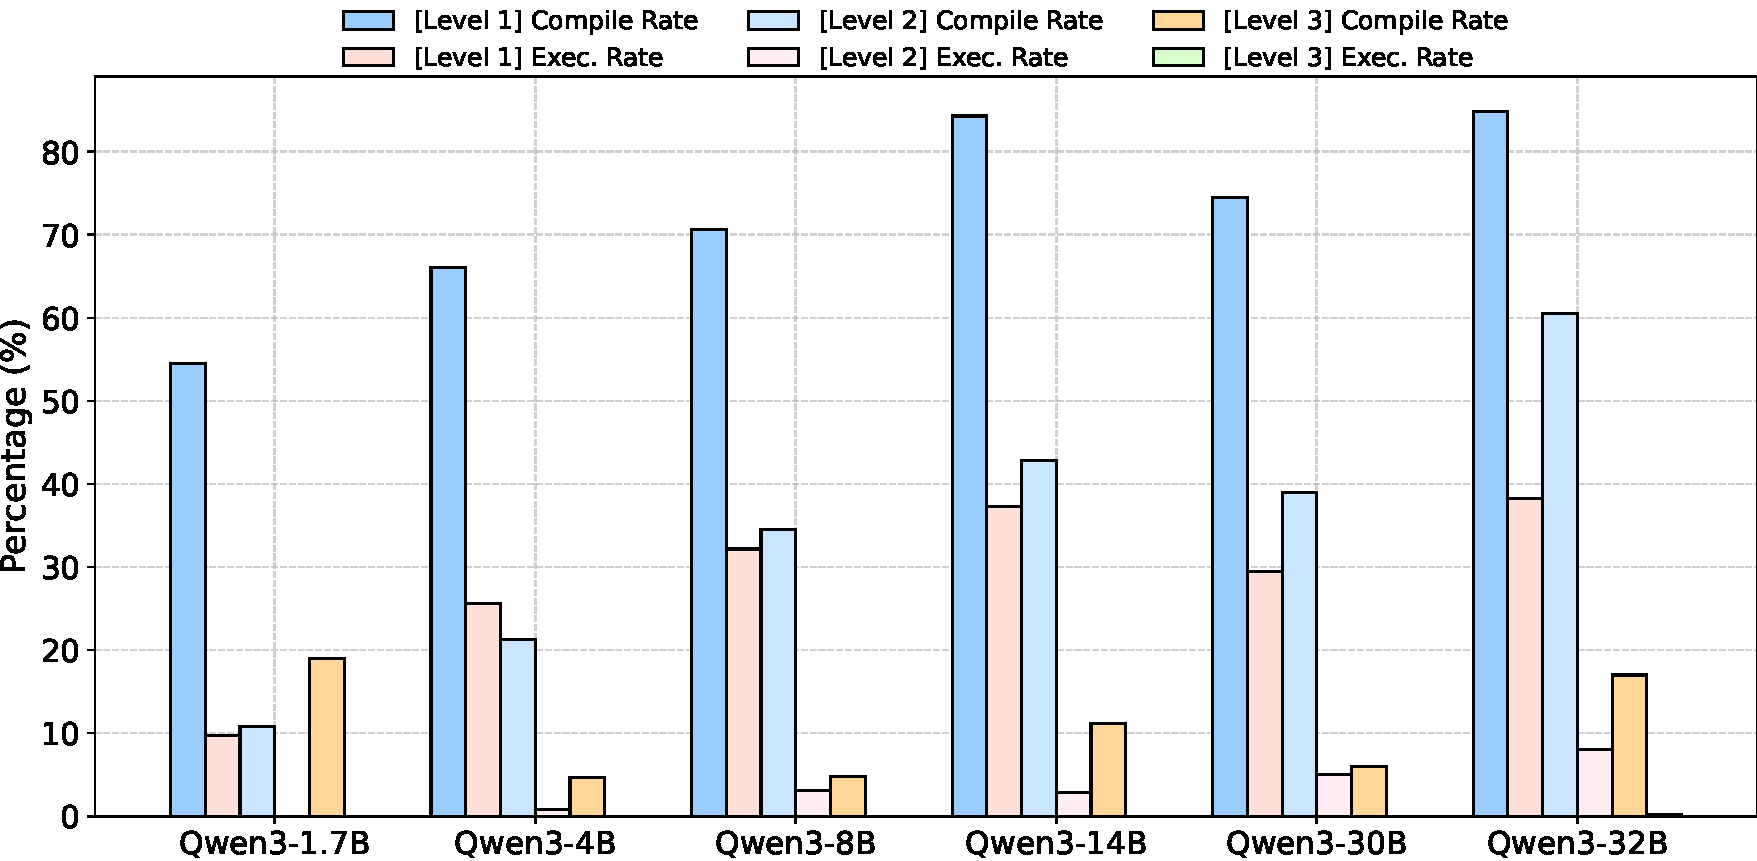
\includegraphics[width=1\linewidth]{pdfs/model_scale.pdf}
    \caption{Scaling behavior of KernelGen-LM on NPU kernel generation tasks with increasing difficulty.}
    \label{fig:model_scale}
\end{figure}

As shown in Figure~\ref{fig:model_scale}, increasing model scale leads to clear performance gains on Level~1 and Level~2 tasks, indicating that larger models better capture standard kernel patterns. In contrast, Level~3 tasks remain highly challenging, with most models failing to achieve non-trivial execution rates. However, 32B is the only scale that demonstrates measurable compilation success on Level~3, suggesting that sufficient parameter scale is a prerequisite for reasoning over the complex control flow and memory dependencies of complicated NPU kernels.

\subsubsection{Comparison of Fine-tuning Strategies}  
% 全量微调与 LoRA 微调策略对比
\begin{table}[t]
    \centering
    \caption{Full-tuning \textit{V.S.} LoRA-tuning in QWen3-8B model.}
    \resizebox{0.75\linewidth}{!}{
    \begin{tabular}{l cc c c}
            \toprule
            \textbf{Model} & \textbf{Level} & \textbf{Compile Rate (\%)} & \textbf{Exec. Rate (\%)} & \textbf{Speedup ($\times$)} \\
            \midrule
            \multirow{4}{*}{LoRA-tuning}  & Level 1   & 54.94 & 20.10  & 0.48 \\  
            & Level 2    & 14.58 & 0.67   & 0.52 \\  
            & Level 3    & 3.83  & 0.00   & - \\ 
            \rowcolor{bggreen}
            & Mean       & 40.29 & 13.55  & 0.48 \\ \hline
             \multirow{4}{*}{Full-tuning}      & Level 1    & 70.67 & 32.17 & 0.58 \\
            & Level 2    & 34.50 & 3.08  & 2.77 \\ 
            & Level 3    & 4.83  & 0.00  & - \\ 
            \rowcolor{bggreen}
            & Mean       & \textbf{55.32} & \textbf{22.13} & \textbf{0.95} \\ 
            \bottomrule
        \end{tabular}
    \label{tab:full_vs_lora}}
\end{table}


Table~\ref{tab:full_vs_lora} compares a comparative analysis between full fine-tuning and LoRA-based fine-tuning on Qwen3-8B.
Full fine-tuning consistently outperforms LoRA across all kernel complexity levels, with the mean compilation rate surging from 40.29\% to 55.32\% and the execution rate improving from 13.55\% to 22.13\%.
The performance gap widens significantly as kernel complexity increases.
We attribute this divergence to the nature of NPU kernel generation, which is a knowledge-intensive task involving strict hardware intrinsics and memory constraints, rather than a simple style transfer.
While LoRA is effective for format alignment, its low-rank decomposition limits the capacity to absorb such high-dimensional, domain-specific knowledge.
In contrast, full fine-tuning updates the entire parameter space, allowing for the deep injection of complex semantics and logical dependencies required for valid code generation.
Consequently, in terms of runtime efficiency, full fine-tuning achieves an average speedup of $0.95\times$, substantially surpassing the $0.48\times$ of LoRA.
These results suggest that for precision-critical tasks like hardware-aware code generation, the comprehensive parameter update of full fine-tuning is indispensable.

\subsubsection{Training Data Composition Analysis} 
% 不同语料来源及数据比例对性能的影响
\begin{figure}[t]
    \centering
    \begin{subfigure}{0.552\textwidth}
        \centering
        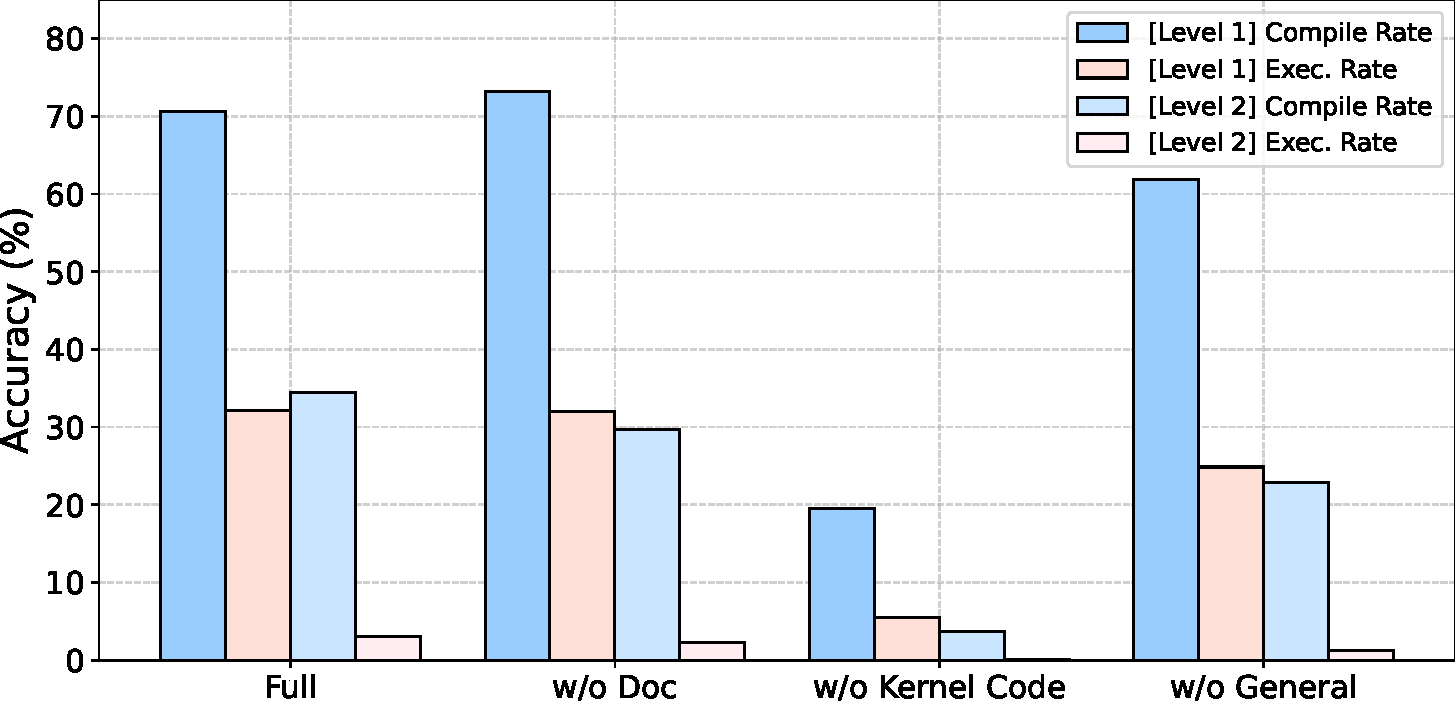
\includegraphics[width=\linewidth]{pdfs/ablation_data_compos.pdf}
        \caption{Pass@1 rates with different data compositions.}
        \label{fig:data_compos}
    \end{subfigure}
    \hfill
    \begin{subfigure}{0.438\textwidth}
        \centering
        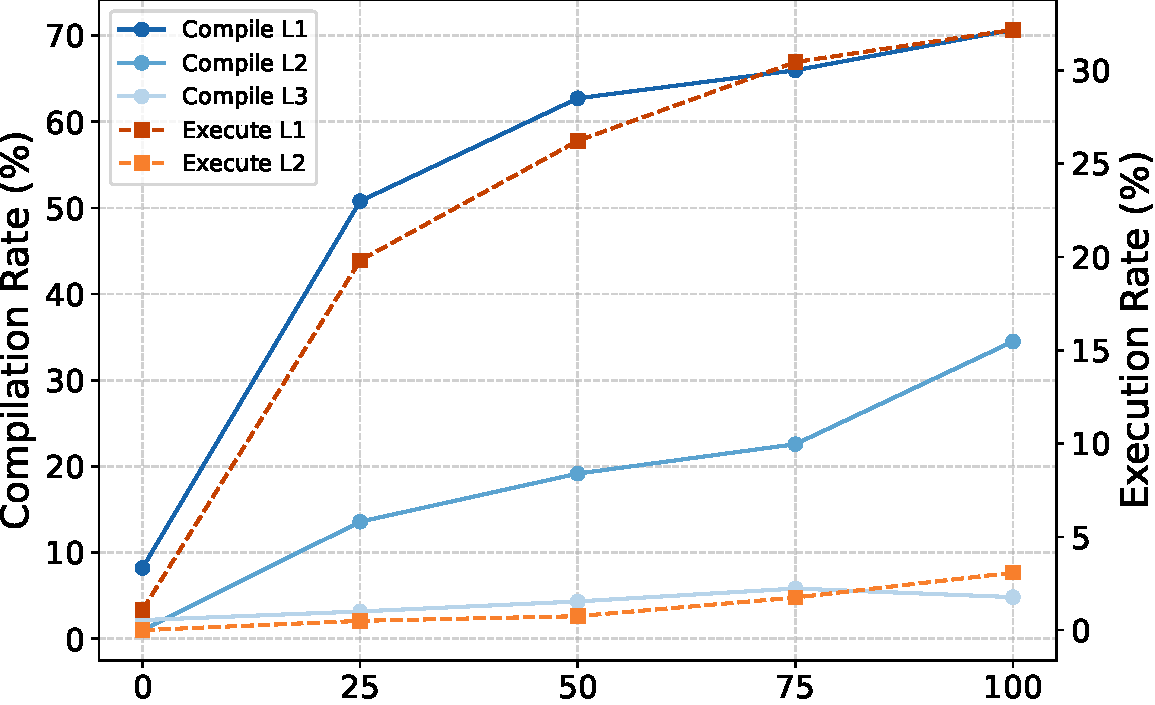
\includegraphics[width=\linewidth]{pdfs/ablation_acc_percent.pdf}
        \caption{Pass@1 rates with varying data ratios in Full setting.}
        \label{fig:data_percent}
    \end{subfigure}
    \caption{Ablation results on training data composition. 
(a) Pass@1 compilation and execution rates for Level~1 and Level~2 kernels on Qwen3-8B under different data composition settings. Removing kernel code leads to the most severe performance degradation, particularly for Level~2 kernels.
(b) Pass@1 compilation and execution rates under the full data setting with different data ratios. Increasing the training data consistently improves both compilation and execution performance.}
    \label{fig:ablation}
\end{figure}

Fig.~\ref{fig:data_compos} shows that removing kernel code from the training data results in a dramatic drop in Pass@1 performance, underscoring its critical role.
Documentation and general semantic data provide auxiliary benefits, particularly for higher-complexity kernels.
Fig.~\ref{fig:data_percent} further demonstrates that increasing the training data size yields consistent improvements, highlighting the importance of data scale.


\subsection{Ablation Analysis of Reinforcement Learning}

\begin{table}[t]
\centering
\caption{DPO hyperparameter ablation in QWen3-8B.}
\resizebox{1\linewidth}{!}{
\begin{tabular}{l c c c c c c}
\toprule
\textbf{Negative Strategy} & \textbf{LR} & \textbf{LR Decay} & \textbf{Batch Size} & \textbf{Training Steps} & \textbf{Compile Rate (\%)} & \textbf{Exec. Rate (\%)} \\
\midrule
 (SFT) & - & - & - & - & \textbf{60.97} & \textbf{5.18}  \\
 \multirow{2}{*}{Compile-pass but execution-fail} 
  &  1e-6 &  constant &  64 &  150 & \textbf{44.21} & \textbf{8.31} \\
  % &  5e-7 &  constant &  128 &  75  & \textbf{56.92}  & \textbf{9.10}  \\
  & 1e-6 &  cosine &  64 &  150  & \textbf{54.03}  & \textbf{9.49}  \\
 Compile-fail &  1e-6 &  constant &  64 &  150 & \textbf{32.00}  & \textbf{6.10} \\
\bottomrule
\end{tabular}
}
\label{tab:DPO_hyper}
\end{table}


Table~\ref{tab:DPO_hyper} presents an ablation study on RL training with different negative strategies and optimization settings, where the negative strategies follow the preference data construction introduced in Sec.~\ref{reinforcement_learning}. Comparing the second row (compile-pass but execution-fail) with the fourth row (compile-fail) shows that using execution-failed yet compilation-passed samples as negatives leads to markedly better compilation and execution performance, indicating that such preference data provides more informative supervision than compile-failed negatives. Under the same negative strategy, a further comparison between the second and third rows demonstrates that cosine learning rate decay consistently outperforms a constant schedule, especially in terms of execution success. These results jointly motivate our choice of execution-failed but compilation-passed samples as negative preferences and cosine decay as the default optimization setting for RL training.

\subsection{Error Analysis}

To better understand the limitations of LLM-based kernel generation, we conduct a systematic error analysis over approximately 4,000 failed kernel generations.
Figure~\ref{fig:placeholder} summarizes the distribution of observed failure types.


\begin{wrapfigure}{r}{0.45\linewidth}
    \centering
    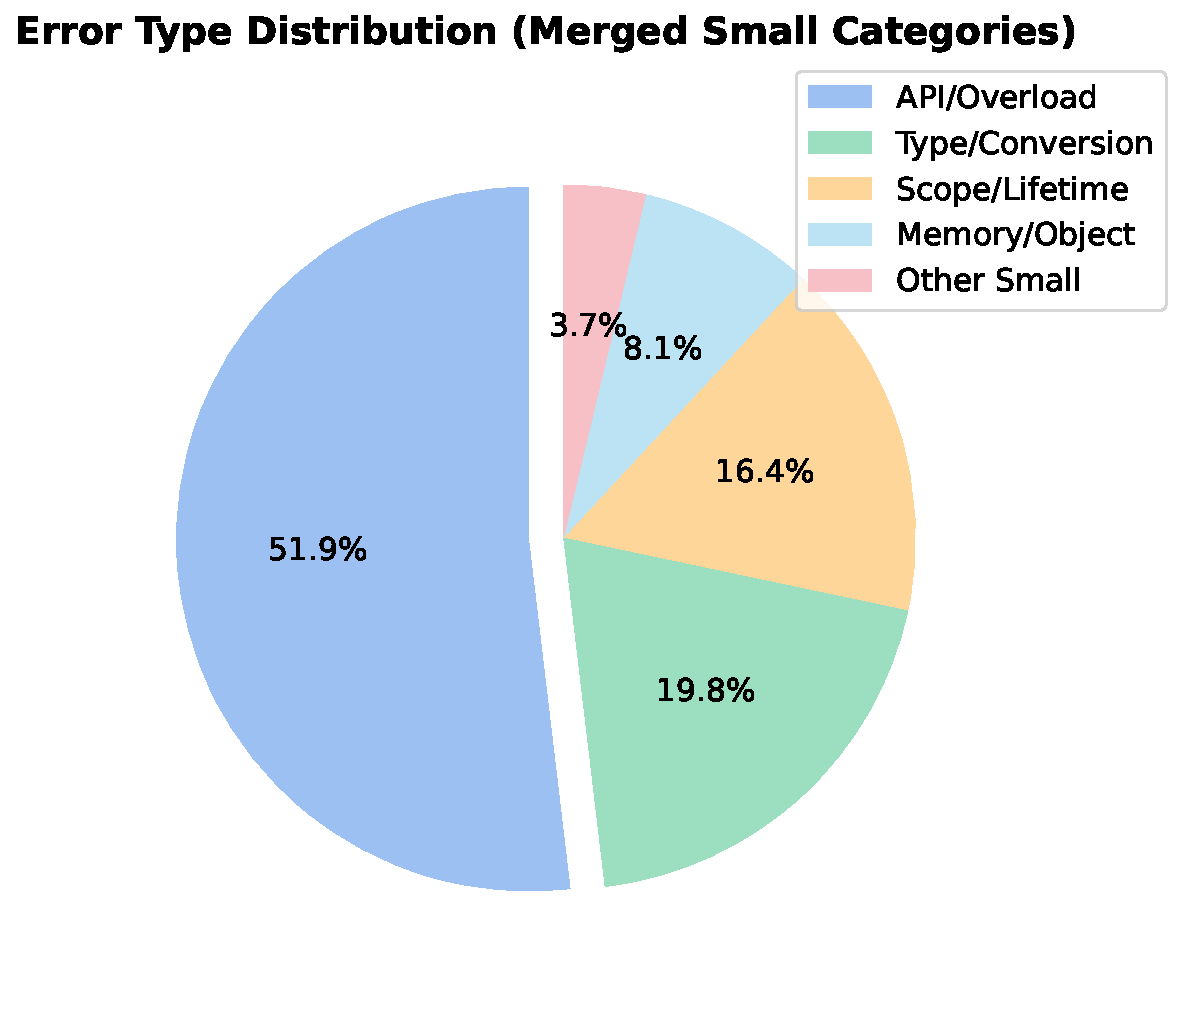
\includegraphics[width=\linewidth]{pdfs/ablation_error_type.pdf}
    \caption{Distribution of kernel generation errors.}
    \label{fig:placeholder}
\end{wrapfigure}

\begin{comment}

Data Type \& Conversion Errors follow, representing 19.8\% of failures and typically arising from type inconsistencies, invalid casting, or shape mismatches.
Variable Scope \& Lifetime Errors constitute 16.4\% of failures, reflecting challenges in correctly managing intermediate buffers, variable lifetimes, and temporary objects.
Finally, the remaining low-frequency errors, including memory \& object usage, syntax \& structure, and macro \& preprocessing errors (combined 3.7\%), are grouped as Other Errors.

\end{comment}

%API Signature and Overload Errors are the most frequent, accounting for 51.9\% of failures, followed by Data Type and Conversion Errors (19.8\%) and Variable Scope and Lifetime Errors (16.4\%). Lower-frequency errors, including memory usage, syntax, and macro-related issues, together account for 3.7\%. These results indicate that while structural and memory-related issues are relatively well handled, generating correct API calls and managing data types and variable scope remain significant challenges for current models.

As shown in the figure, API Signature and Overload Errors constitute the dominant failure mode, accounting for 51.9\% of all failed cases. These errors occur when generated function invocations fail to match any valid AscendC API signature or overload. The second most common category is Data Type and Conversion Errors (19.8\%), followed by Variable Scope and Lifetime Errors (16.4\%) and Memory and Object Usage Errors (8.1\%). Lower-frequency failures—including syntax and structural violations as well as macro and preprocessing errors—together account for only 3.7\% of all cases.

\begin{comment}

The most prevalent failure mode corresponds to API signature and overload errors, accounting for 51.9\% of all failures.
These errors arise when generated function invocations do not match any valid AscendC API signature.
The next most frequent categories include data type and conversion errors (19.8\%) and variable scope and lifetime errors (16.4\%).
In contrast, errors related to syntax, memory usage, and macro preprocessing are relatively rare, jointly contributing only 3.7\% of the total failures.

This distribution reveals a clear pattern: while current models are generally capable of producing syntactically valid kernel structures and managing basic memory operations, they struggle with semantically constrained reasoning, particularly in API invocation, type consistency, and program state management.

\end{comment}

%In the following, we analyze the major error categories to understand their underlying causes and implications for LLM-based kernel generation.
%Overall, the observed failures can be grouped into three high-level error modes, reflecting limitations in API reasoning, low-level type handling, and program state management.

This distribution indicates that current models are generally capable of producing syntactically well-formed kernel code, as purely syntactic and structural errors are relatively rare.
However, the majority of failures arise from semantically constrained aspects of low-level programming.
In particular, errors are dominated by cases that require precise reasoning about API contracts, hardware-specific data types, and variable visibility across different kernel components.

To further investigate the underlying causes of these failures, we analyze the major error categories in detail. Below, we describe each error category along with its typical causes and manifestations.

\begin{comment}

Based on these observations, we cluster the failures into three high-level error modes that reflect fundamental reasoning limitations in low-level kernel generation.
First, \emph{API reasoning errors} occur when the model fails to align function arguments with hardware-specific API contracts, leading to invalid overload resolution.
Second, \emph{type-level reasoning errors} stem from improper handling of low-level data types and implicit conversions, which are especially error-prone in performance-critical kernel code.
Third, \emph{program state management errors} arise from incorrect assumptions about variable scope, lifetime, or visibility across host–kernel boundaries.

Less frequent failure modes, including memory object misuse, syntactic inconsistencies, and macro-related issues, can be largely attributed to incomplete code generation or template misalignment rather than fundamental reasoning gaps.
Representative examples of each error category are provided in Table~\ref{tab:error_examples} in the Appendix.

\end{comment}

\begin{itemize}
    \item \textbf{API Signature \& Overload Errors}: These errors arise when a generated function call does not match any valid API signature or overload defined in the programming interface. Common causes include incorrect argument ordering, mismatched parameter types, missing required parameters, or confusion between similarly named APIs with subtle semantic differences. This category reflects the model’s difficulty in aligning high-level task intent with rigid, hardware-specific API contracts.
    
    \item \textbf{Data Type \& Conversion Errors}: This category includes the use of invalid or non-existent data types (e.g., \texttt{bool\_t}), as well as illegal or unsafe type conversions between incompatible types (e.g., mixing \texttt{float} and \texttt{double} constants). Such errors often stem from implicit assumptions carried over from high-level programming languages, which do not hold in low-level kernel development where type rules are strict and hardware-dependent.

    \item \textbf{Variable Scope \& Lifetime Errors}: These errors occur when variables are used outside their valid scope or before being properly defined. Typical examples include references to undeclared symbols (e.g., \texttt{M\_PI}) or misuse of variables that are not visible within the current compilation unit or kernel context. This category highlights challenges in consistently reasoning about variable visibility and lifetime across host-side logic, kernel code, and auxiliary configuration structures.
    
    \item \textbf{Memory \& Object Usage Errors}: Errors in this category are related to incorrect usage of core objects such as \texttt{TPipe}, \texttt{LocalTensor}, and \texttt{GlobalTensor}. They include invalid member function invocations and incorrect memory address computations. While less frequent, such errors can lead to severe runtime failures or undefined behavior.

    \item \textbf{Syntax \& Structure Errors}: These errors stem from violations of C++ syntax or incomplete kernel class definitions. Examples include missing required methods (e.g., improperly defined or absent \texttt{Init} functions), mismatched braces, or malformed template instantiations.
    These errors are typically associated with incomplete code generation rather than deeper semantic misunderstandings.

    \item \textbf{Macro \& Preprocessing Errors}: This category includes errors caused by incorrect macro definitions or improper usage of tiling-related preprocessing directives. These issues often arise from incorrect assumptions about compile-time constants or conditional compilation logic embedded in kernel templates.

\end{itemize}

\begin{comment}

\begin{itemize}
    \item \textbf{API-Level Reasoning Errors.}
    The most prevalent failures arise from incorrect API usage, including signature mismatches and overload resolution errors.
    Although the generated code often appears syntactically plausible, the arguments do not conform to any valid API signature.
    This indicates that current models struggle to precisely align function semantics with hardware-specific API contracts.

    \item \textbf{Type System and Data Representation Errors.}
    A substantial portion of failures are caused by invalid data types or illegal type conversions, such as the use of unsupported types (e.g., \texttt{bool\_t}) or inconsistent constant types (\texttt{float} vs.\ \texttt{double}).
    These errors suggest limited robustness in modeling low-level type systems and numeric constraints imposed by NPU kernels.

    \item \textbf{Program State and Structural Errors.}
    The remaining failures are related to incorrect management of program state, including variable scope and lifetime errors, improper memory or object usage involving \texttt{TPipe}, \texttt{LocalTensor}, and \texttt{GlobalTensor}, as well as syntax, class structure, and macro preprocessing issues.
    While individually less frequent, these errors highlight challenges in generating globally consistent and executable kernel programs.
\end{itemize}

\end{comment}

Representative examples for each error category are provided in Table~\ref{tab:error_examples} in the Appendix.
\section{Conclusion}
\label{conclusions}

In this work, we presented Ascend KernelGen, a unified framework designed to automate the generation of high-performance kernels for NPU architectures. We identified that the primary barrier for LLMs in this domain is not merely syntax familiarity, but the lack of structured reasoning capabilities regarding hardware constraints, memory hierarchy management, and asynchronous pipeline synchronization.

To overcome this, we constructed Ascend-CoT, a domain-specific dataset that explicitly models the reasoning process of expert developers, and developed NPUKernelBench, a rigorous evaluation suite that goes beyond static code analysis to verify compilation, numerical correctness, and runtime performance on actual hardware. Our extensive experiments show that while general-purpose models struggle with the specificity of AscendC, our domain-adaptive training strategy—combining reasoning-oriented supervised fine-tuning with execution-guided reinforcement learning—yields substantial improvements. We demonstrated that our model can successfully generate complex operators that were previously out of reach, achieving competitive performance metrics.

While this study focuses on kernel-level correctness and basic optimization, several promising directions remain. First, we plan to extend our framework to better support Level-3 kernels, which remain challenging for current models. Second, we aim to integrate performance-aware reward models into the reinforcement learning stage to prioritize not just functional correctness, but also latency minimization and resource utilization close to the hardware roofline. Finally, we intend to explore the generalizability of our methodology to other emerging accelerator platforms, fostering a more inclusive ecosystem for AI-driven hardware software co-design.
\clearpage
% !htbp
\begin{table}[t]
  \centering
  % ============================= Outer container (single prompt)
  \begin{tcolorbox}[
    rounded corners,
    arc=3pt,
    enhanced,
    width=1\textwidth,
    colframe=refpurple!15, % <----- CHANGED
    coltitle=refpurple,
    colback=white,
    title=\textbf{Evaluation Criteria},
    fonttitle=\bfseries\small,
    boxrule=0.6pt,
    left=2pt,
    right=2pt,
    top=0pt,
    bottom=1pt
  ]
% --------------- Part 2: Previous CUDA implement with scores
\begin{tcolorbox}[
      sharp corners,
      colframe=refgreen,
      colback=refgreen!5,
      colbacktitle=refgreen!15,
      coltitle=refgreen,
      boxrule=0.4pt,
      title={\textbf{Default evaluation criteria}},
      fonttitle=\bfseries\small,
      left=0pt,
      right=0pt,
      top=-4pt,
      bottom=-4pt
    ]
      \begin{center}
        \begin{lstlisting}[style=mystyle, frame=none,framerule=0pt, language=Python]
def check_precision(outputs, outputs_new, max_abs_error, max_rel_error):
    # outputs: list of tensors from reference model
    # outputs_new: list of tensors from LLM generated kernel
    outputs = [outputs] if not isinstance(outputs, list) else outputs
    outputs_new = [outputs_new] if not isinstance(outputs_new, list) else outputs_new
    
    all_abs_diff, all_rel_diff = [], []
    is_accurate = True
    
    # Process each output pair
    for out, out_new in zip(outputs, outputs_new):
      abs_diff = torch.abs(out - out_new)
      rel_diff = abs_diff / (torch.abs(out) + 1e-7) # Add epsilon to avoid division by zero
      all_abs_diff.append(abs_diff.view(-1))
      all_rel_diff.append(rel_diff.view(-1))
    
      # Check if any element exceeds both absolute and relative error thresholds
      if ((abs_diff > max_abs_error) & (rel_diff > max_rel_error)).any():
          is_accurate = False
    
    # Combine all differences
    all_abs_diff = torch.cat(all_abs_diff)
    all_rel_diff = torch.cat(all_rel_diff)
    
    return (1 if is_accurate else 0), all_abs_diff, all_rel_diff
\end{lstlisting}
\end{center}
\end{tcolorbox}

\begin{tcolorbox}[
      sharp corners,
      colframe=refgreen,
      colback=refgreen!5,
      colbacktitle=refgreen!15,
      coltitle=refgreen,
      boxrule=0.4pt,
      title={\textbf{Custom evaluation criteria}},
      fonttitle=\bfseries\small,
      left=0pt,
      right=0pt,
      top=-4pt,
      bottom=-5pt
    ]
      \begin{center}
        \begin{lstlisting}[style=mystyle, frame=none,framerule=0pt, language=Python,upquote=true]
def custom_check_precision(param, outputs, outputs_new):
    dtype_str = param.get(`dtype`, `float16`)
    dtype = getattr(torch, dtype_str)
    if dtype == torch.float32:
        return check_precision(outputs, outputs_new, max_abs_error=0.00001, max_rel_error=0.00001)
    else:
        return check_precision(outputs, outputs_new, max_abs_error=0.001, max_rel_error=0.001)
\end{lstlisting}
\end{center}
\end{tcolorbox}
\end{tcolorbox}
\vspace{-10pt}
\caption{Correctness evaluation criteria for LLM-generated kernels, covering both default and custom methods.}
\label{tab:kernel_correctness}
\end{table}




% !htbp
\begin{table}[H]

  \centering
  % ============================= Outer container (single prompt)
  \begin{tcolorbox}[
    rounded corners,
    arc=3pt,
    enhanced,
    width=1\textwidth,
    colframe=codegreen, % <----- CHANGED
    colback=white,
    title=\textbf{Prompts for Generating Kernel Code in NPUKernelBench},
    fonttitle=\bfseries\small,
    boxrule=0.6pt,
    left=2pt,
    right=2pt,
    top=0pt,
    bottom=1pt
  ]
    \begin{tcolorbox}[
      sharp corners,
      colframe=reforange,
      colback=reforange!5,
      colbacktitle=reforange!15,
      coltitle=reforange,
      boxrule=0.4pt,
      title={\textbf{Instructions}},
      fonttitle=\bfseries\small,
      left=0.5pt,
      right=0.5pt,
      top=0.5pt,
      bottom=0.5pt
    ]
{\small Please see Table~\ref{tab:prompt_ins}.}
\end{tcolorbox}

\begin{tcolorbox}[
      sharp corners,
      colframe=taskblue,
      colback=taskblue!5,
      colbacktitle=taskblue!15,
      coltitle=taskblue,
      boxrule=0.4pt,
      title={\textbf{API\_Desc.md}},
      fonttitle=\bfseries\small,
      left=0pt,
      right=0pt,
      top=0pt,
      bottom=0pt
    ]
\begin{lstlisting}[style=mdstyle]
# aclnnBasicMatmul 
## Function Description 
### Kernel Function 
This Ascend C kernel performs the multiplication of two 2D matrices, A and B. It is a core component in deep learning models, such as linear layers and attention mechanisms. It takes two 2D tensors that satisfy the matrix multiplication rule and outputs their product.
### Computational Formula 
Assume the input tensors are $A$ ($m \times k$) and $B$ ($k \times n$). The output tensor $C$ ($m \times n$) is computed as: $$C_{ij} = \sum_{p=1}^{k} A_{ip} B_{pj}$$, where $i$ ranges from $1$ to $m$, and $j$ ranges from $1$ to $n$. $C_{ij}$ denotes the element in the $i$-th row and $j$-th column of $C$.
### Computation Process and Type Conversion
To maintain high numerical precision during large-scale accumulation and effectively prevent data overflow, this kernel adopts a high-precision accumulation strategy during computation. The process is as follows: 
1. The kernel receives two input tensors  `a` and `b`, both of data type `float16`.
2. During the multiply-accumulate computation, the internal accumulator uses the `float32` data type. In other words, the product results of `float16` inputs are first converted to `float32` before accumulation.
3. After all accumulation operations are completed, a result tensor of type `float32` is obtained.
4. Finally, the `float32` result tensor is converted back to `float16` as the final output.
## Interface Definition
### Kernel Prototype Definition Interface
#### Input 
- a: Device-side aclTensor corresponding to A in the formula; supports float16, 2D, and ND format.
- b: Device-side aclTensor corresponding to B in the formula; supports float16, 2D, and ND format.
#### Output 
- c: Device-side aclTensor corresponding to C in the formula; supports float16, 2D, and ND format.
#### Attr 
- None
## Constraints and Limitations
* The input tensors `a` and `b` currently support only the `float16` data type.
* The input tensors `a` and `b` must both be two-dimensional matrices.
* The second dimension (number of columns) of `a` must be equal to the first dimension (number of rows) of `b`.
* The input tensors support only the ND data format.
\end{lstlisting}
 \end{tcolorbox}
 
% --------------- Part 2: Previous CUDA implement with scores
\begin{tcolorbox}[
      sharp corners,
      colframe=refgreen,
      colback=refgreen!5,
      colbacktitle=refgreen!15,
      coltitle=refgreen,
      boxrule=0.4pt,
      title={\textbf{Host template}},
      fonttitle=\bfseries\small,
      left=0pt,
      right=0pt,
      top=-4pt,
      bottom=-4pt
    ]
      \begin{center}
        \begin{lstlisting}[style=mystyle, frame=none,framerule=0pt, language=Python]
#include "register/op_def_registry.h" 
#include "tiling/platform/platform_ascendc.h" 
namespace optiling { 
static ge::graphStatus TilingFunc(gert::TilingContext *context) 
{ 
    context->SetBlockDim(platform_ascendc::PlatformAscendCManager::GetInstance()->GetCoreNumAic()); 
    return ge::GRAPH_SUCCESS; 
} 
} // namespace optiling 
namespace ops { 
class BasicMatmul : public OpDef { 
public: 
    explicit BasicMatmul(const char *name) : OpDef(name) 
{ 
        this->Input("a") 
            .ParamType(REQUIRED) 
            .DataType({ge::DT_FLOAT16}) 
            .Format({ge::FORMAT_ND}); 
        this->Input("b") 
            .ParamType(REQUIRED) 
            .DataType({ge::DT_FLOAT16}) 
            .Format({ge::FORMAT_ND}); 
        this->Output("c") 
            .ParamType(REQUIRED) 
            .DataType({ge::DT_FLOAT16}) 
            .Format({ge::FORMAT_ND}); 
        this->AICore() 
            .SetTiling(optiling::TilingFunc) 
            .AddConfig("ascend910_93") 
            .AddConfig("ascend910b"); 
    } 
}; 
OP_ADD(BasicMatmul); 
} // namespace ops
\end{lstlisting}
\end{center}
\end{tcolorbox}

\begin{tcolorbox}[
      sharp corners,
      colframe=refgreen,
      colback=refgreen!5,
      colbacktitle=refgreen!15,
      coltitle=refgreen,
      boxrule=0.4pt,
      title={\textbf{Kernel template}},
      fonttitle=\bfseries\small,
      left=0pt,
      right=0pt,
      top=-4pt,
      bottom=-5pt
    ]
      \begin{center}
        \begin{lstlisting}[style=mystyle, frame=none,framerule=0pt, language=Python]
#include <kernel_operator.h> 
using namespace AscendC; 
extern "C" __global__ __aicore__ void basic_matmul(GM_ADDR a, GM_ADDR b, GM_ADDR c, GM_ADDR workspace, GM_ADDR tiling) 
{ 
}
\end{lstlisting}
\end{center}
\end{tcolorbox}
\end{tcolorbox}
\vspace{-10pt}
\caption{An example of the structured prompt used for Ascend kernel generation, consisting of three components: API description, host/kernel-side template.}
\label{tab:kernel_gen}
\end{table}



\begin{table*}
\centering
    \begin{tcolorbox}[
    breakable,
      sharp corners,
      colframe=refpurple,
      colback=refpurple!5,
      colbacktitle=refpurple!15,
      coltitle=refpurple,
      boxrule=0.4pt,
      title={Kernel-level CoT}, 
      fonttitle=\bfseries\small,
      left=0.5pt,
      right=0.5pt,
      top=0.5pt,
      bottom=0.5pt
    ]

% 使用自定义样式
\begin{lstlisting}[language=json]
{
  "qus": "Please implement a utility function for computing the temporary buffer size required by the SwiGLU operator. The function should be able to determine the maximum and minimum buffer sizes based on the input shape and data type, as well as retrieve the buffer’s factor size. Some dependency code has already been provided; please complete the implementation based on the following summarized dependencies: [==========From swiglu\_tiling.h ==================...code...================== From /api\_check/host\_apicheck.h =======...code...==================== From impl/host\_log.h ======================...code...]",
  "cot": "To solve this problem, I need to implement a utility function that computes the temporary buffer size required by the SwiGLU operator. The function must determine the maximum and minimum buffer sizes based on the input shape and data type, as well as return the buffer-size factor. According to the provided dependency code, basic interfaces and parameter-validation utilities already exist, so my task is to implement the core logic. Since SwiGLU requires intermediate results, its temporary-space needs vary across data types, and the Ascend processor also imposes alignment constraints, motivating the use of a minimum repeat-unit size. My design sets different multipliers for half-precision and single-precision data, defines a 256-byte minimum repeat unit, and validates both shape and datatype. The maximum buffer size is computed as the multiplier times the larger of the input-tensor byte size and the repeat-unit size, while the minimum buffer size uses only the repeat-unit size. The factor-size interface simply returns the chosen multiplier, enabling callers to compute the exact temporary-space requirement dynamically.",
  "ans": "/* !\n * \\file swiglu_tiling.cpp\n * \\brief\n */\n# include \"lib/activation/swiglu_tiling.h\"\n\n#include <cstdint>\n#include <set>\n\n#include \"graph/tensor.h\"\n#include \"impl/host_log.h\"\n#include \"impl/api_check/host_apicheck.h\"\n\nnamespace AscendC {\nnamespace {\nconstexpr uint32_t SWIGLU_HALF_TMP_SIZE = 6;\nconstexpr uint32_t SWIGLU_FLOAT_TMP_SIZE = 0;\nconstexpr uint32_t SWIGLU_ONE_REPEAT_BYTE_SIZE = 256;\nstatic constexpr uint32_t SWI_GELU_HALF_SIEZ = 2;\nstatic constexpr uint32_t SWI_GELU_FLOAT_SIEZ = 4;\nstatic const std::set<uint32_t> SUPPORT_TYPESIZE = { SWI_GELU_HALF_SIEZ, SWI_GELU_FLOAT_SIEZ };\nstatic constexpr const char SWI_GELU_GET_MAX_MIN[] = \"GetSwiGLUMaxMinTmpSize\";\nstatic constexpr const char SWI_GELU_GET_TMP_BUFFER[] = \"GetSwiGLUTmpBufferFactorSize\";\n\ninline uint32_t GetSwiGLUMaxTmpSize(const uint32_t inputSize, const uint32_t typeSize)\n{\n    const uint32_t calcPro = (typeSize == sizeof(float)) ? SWIGLU_FLOAT_TMP_SIZE : SWIGLU_HALF_TMP_SIZE;\n    return calcPro * std::max(inputSize * typeSize, SWIGLU_ONE_REPEAT_BYTE_SIZE);\n}\n\ninline uint32_t GetSwiGLUMinTmpSize(const uint32_t typeSize)\n{\n    const uint32_t calcPro = (typeSize == sizeof(float)) ? SWIGLU_FLOAT_TMP_SIZE : SWIGLU_HALF_TMP_SIZE;\n    return calcPro * SWIGLU_ONE_REPEAT_BYTE_SIZE;\n}\n} // namespace\n\nvoid GetSwiGLUMaxMinTmpSize(const ge::Shape& srcShape, const uint32_t typeSize, uint32_t& maxValue,\n    uint32_t& minValue, const bool isReuseSource)\n{\n    HighLevelApiCheck::SrcShapeSizeVerifyingParameters<SWI_GELU_GET_MAX_MIN>(srcShape.GetShapeSize(), typeSize);\n    HighLevelApiCheck::TypeSizeVerifyingParameters<SWI_GELU_GET_MAX_MIN>(typeSize, SUPPORT_TYPESIZE);\n    HighLevelApiCheck::IsReuseSourceVerifyingParameters<SWI_GELU_GET_MAX_MIN>(isReuseSource);\n    const uint32_t inputSize = srcShape.GetShapeSize();\n    ASCENDC_HOST_ASSERT(inputSize > 0, return, \"Input Shape size must be greater than 0.\");\n\n    minValue = GetSwiGLUMinTmpSize(typeSize);\n    maxValue = GetSwiGLUMaxTmpSize(inputSize, typeSize);\n}\n\nvoid GetSwiGLUTmpBufferFactorSize(const uint32_t typeSize, uint32_t &maxLiveNodeCount, uint32_t &extraBuffer)\n{\n    HighLevelApiCheck::TypeSizeVerifyingParameters<SWI_GELU_GET_TMP_BUFFER>(typeSize, SUPPORT_TYPESIZE);\n    extraBuffer = 0;\n    maxLiveNodeCount = (typeSize == sizeof(float)) ? SWIGLU_FLOAT_TMP_SIZE : SWIGLU_HALF_TMP_SIZE;\n}\n} // namespace AscendC"
}
\end{lstlisting}
\end{tcolorbox}
\vspace{-10pt}
\caption{A SwiGLU kernel CoT example for Ascend kernel SFT, consisting of three parts: question, CoT, and answer.}
\label{tab:singel_example}
\end{table*}
\begin{tcolorbox}[
    breakable,
    rounded corners,
    arc=3pt,
    enhanced,
    width=1\textwidth,
    colframe=codegreen, % <----- CHANGED
    colback=white,
    title=\textbf{Prompt for generating project-level CoT},
    fonttitle=\bfseries\small,
    boxrule=0.6pt,
    left=2pt,
    right=2pt,
    top=0pt,
    bottom=1pt
  ]
    \begin{tcolorbox}[
      sharp corners,
      colframe=reforange,
      colback=reforange!5,
      colbacktitle=reforange!15,
      coltitle=reforange,
      boxrule=0.4pt,
      title={\textbf{Instructions}},
      fonttitle=\bfseries\small,
      left=0.5pt,
      right=0.5pt,
      top=0.5pt,
      bottom=0.5pt
    ]
{\small 
You are an AscendC programming expert for the Huawei Ascend processor. Based on the given problem, code content, and hardware specification documentation, please generate a detailed chain-of-thought process and a summary of all member variable values within the structures, as well as the value of the tilingKey.
The chain of thought should demonstrate the complete reasoning path from the problem to the final code outcome, including key thinking steps, logical analysis, and derivation.

Requirements:

Start reasoning from the problem itself, with reasoning details aligned with the implementation logic;

Present a clear solution path;

Include necessary analytical steps and intermediate reasoning;

Guide the reasoning process step by step toward the final answer;

Demonstrate your expertise and reasoning process as an AscendC specialist;

......

For the chain of thought, the following requirements apply:

1. Begin from the problem and reason in the first-person “I”.

2. Present yourself as a developer actively solving the problem, not as an AI that already knows the answer.

3. Show the natural thought process from problem analysis to solution design and then to implementation. Code snippets may only reproduce content from the given material and must not be invented. Avoid statements such as “based on the example”.

4. Include key decision points, technical considerations, and derivations.

......

11. Except for code and proper nouns, do not use English inside the internal reasoning process (chain of thought itself).

12. Tiling parameters mainly include the following components:

    - {BlockDim}: the value set by the \texttt{GetBlockDim()} function
    
    - {TilingKey}: the value set by the \texttt{SetTilingKey()} function (optional)
    
    - {Tiling structure member variables}: typically defined between
      \texttt{BEGIN\_TILING\_DATA\_DEF()} and \texttt{END\_TILING\_DATA\_DEF()} in \texttt{*\_tiling.h}
    
......


The chain of thought should be output in the following format:

\texttt{<think>chain-of-thought</think}
.}
\end{tcolorbox}

\begin{tcolorbox}[
      sharp corners,
      colframe=taskblue,
      colback=taskblue!5,
      colbacktitle=taskblue!15,
      coltitle=taskblue,
      boxrule=0.4pt,
      title={\textbf{Test cases}},
      fonttitle=\bfseries\small,
      left=0pt,
      right=0pt,
      top=0pt,
      bottom=0pt
    ]
\begin{lstlisting}[style=mdstyle]
## Function Description
### Operator Function
Returns a new tensor with the same shape as the input, where each element is the absolute value of the corresponding input element.
### Formula
$$
x = [x_0, x_1, \ldots, x_{n-1}] \\
y = [y_0, y_1, \ldots, y_{n-1}]
$$
$$
y_i = |x_i|,\quad i = 0, 1, \ldots, n-1
$$
## API Definition
### Python API
This operator is implemented in C++ and exposed to Python via PyBind11 as `kernel_gen_ops.abs_math()`:
```python
def abs_math(tensor):
    """
    Custom AbsMath operator.

    Args:
        tensor (Tensor): Device-side aclTensor (input x).
            Supported dtypes: bfloat16, float16, float32, int32, int64, DT_COMPLEX64.
            Supported format: ND.

    Returns:
        Tensor: Device-side aclTensor (output y).
            Same dtype/format as input. Output shape matches x.
    """
```
## Usage Example
```python
import torch
import kernel_gen_ops

tensor = torch.tensor([-1.0, 2.0, -3.0], dtype=torch.float)
result = kernel_gen_ops.abs_math(tensor)
```
## Constraints
- ND format only.
\end{lstlisting}
 \end{tcolorbox}
 
% --------------- Part 2: 
\begin{tcolorbox}[
      sharp corners,
      colframe=refgreen,
      colback=refgreen!5,
      colbacktitle=refgreen!15,
      coltitle=refgreen,
      boxrule=0.4pt,
      title={\textbf{NPUs hardware configuration}},
      fonttitle=\bfseries\small,
      left=0pt,
      right=0pt,
      top=-4pt,
      bottom=-4pt
    ]
      \begin{center}
        \begin{lstlisting}[style=mdstyle]
The introductory document for AscendC development includes the following sections:
1. Overview of the Decoupled Architecture and Hardware Structure
1.1 Features of the Decoupled Architecture
The decoupled architecture of Ascend AI processors (e.g., Atlas A2/A3 series) splits the AI Core into two independent units: AI Cube (AIC) and AI Vector (AIV).
AIC mainly handles matrix operations (Cube), while AIV is responsible for vector and scalar operations (Vector/Scalar).
The two types of cores have independent scalar units, instruction streams, and local storage. Data is exchanged through Global Memory (GM).
......
The hardware model and specifications we are using are: [Platform Info configuration begin]
#*************************************************************************************#
[
[version]
SoC_version=Ascend910_9392
Short_SoC_version=Ascend910_93   [PS: Ascend910_93 is the NPU's name.]
AIC_version=AIC-C-220
CCEC_AIC_version=dav-c220-cube
CCEC_AIV_version=dav-c220-vec
CCEC_CUBE_version=dav-c220-cube
CCEC_VECTOR_version=dav-c220-vec
......
]

\end{lstlisting}
\end{center}
\end{tcolorbox}

\begin{tcolorbox}[
      sharp corners,
      colframe=refgreen,
      colback=refgreen!5,
      colbacktitle=refgreen!15,
      coltitle=refgreen,
      boxrule=0.4pt,
      title={\textbf{Kernel source code}},
      fonttitle=\bfseries\small,
      left=0pt,
      right=0pt,
      top=-4pt,
      bottom=-5pt
    ]
      \begin{center}
        \begin{lstlisting}[style=mdstyle]
Please, using the input shapes and other relevant information and taking the actual code implementation into account, outline the detailed design logic for operator tiling and kernel pipelining, and compute the operator’s tiling parameter values during the intermediate steps. Below is the code, consisting of multiple files separated by
============================================================================================.
You may refer to these files to support your reasoning, but they are only supplementary. Your answer should be based on your own thinking and judgment as an AscendC expert, not a verbatim restatement of the code:
============================================================================================
```cpp
// op_host/abs_tiling.h
/**
 * @file abs_tiling.h
 */
#ifndef ABS_TILING_H
#define ABS_TILING_H
#include "register/tilingdata_base.h"
namespace optiling {
    ......
}
#endif // ADD_CUSTOM_TILING_H
```
==========================================================================================
```cpp
// op_host/abs_math.cpp
/**
 * @file abs.cpp
 */
#include "abs_tiling.h"
#include "register/op_def_registry.h"
#include "tiling/platform/platform_ascendc.h"
namespace optiling {      
    ......
}
namespace ops {
class AbsMath : public OpDef {
    ......
};OP_ADD(AbsMath);
}
```
==========================================================================================
```cpp
// op_kernel/abs_common.h
/**
 * @file abs_common.h
 */
#ifndef ABS_COMMON_H
#define ABS_COMMON_H
#include "kernel_operator.h"
constexpr int32_t BUFFER_NUM = 2; // tensor num for each queue
#endif // ABS_COMMON_H
    ......
```
==========================================================================================
\end{lstlisting}
\end{center}
\end{tcolorbox}
\end{tcolorbox}
\vspace{-10pt}
\captionof{table}{An example of an AbsMath kernel prompt for Ascend kernel generation, comprising four components: instruction text, test cases, NPU hardware configuration, and kernel source code.}
\label{tab:prompt_project_file}
\clearpage
% \clearpage
% !htbp
\begin{table}[t]
  \centering
  % ============================= Outer container (single prompt)
    \begin{tcolorbox}[
    breakable,
      sharp corners,
      colframe=refpurple,
      colback=refpurple!5,
      colbacktitle=refpurple!15,
      coltitle=refpurple,
      boxrule=0.4pt,
      title={Project-level CoT}, 
      fonttitle=\bfseries\small,
      left=0.5pt,
      right=0.5pt,
      top=0.5pt,
      bottom=0.5pt
    ]

% 使用自定义样式
\begin{lstlisting}[language=json]
{
 "input": "Prompt in Table 9.",
 "output": "<think>\n My task is to implement an `AbsMath` operator for the Ascend processor. The operator's function is simple: take the absolute value of each element of the input tensor, i.e., `y = |x|`.\n\n First, let's analyze its characteristics. It is a typical element-wise operation with simple logic, no complex dependencies, and no matrix multiplication. Therefore, it is vector-intensive, meaning on the Ascend processor, I should mainly use the AI Vector (AIV) units rather than AI Cube (AIC) units.\n\nThe hardware model is `Ascend910_93` with `vector_core_cnt=48` Vector cores. Each core has a Unified Buffer (UB) of 196,352 bytes. UB size limits the amount of data that can be processed at once. The input is `shape=[1]`, `dtype=float16`. Though very small, the implementation (especially tiling) must handle arbitrary sizes. Based on this, the implementation is divided into Host-side Tiling logic and Device-side Kernel.\n\n**I. Host-side Tiling Strategy Design**\n\nThe core goal of Tiling is to decompose the entire computation task into small tiles so that it can be processed in parallel on multiple cores and ensure that each data block can be loaded into UB. \n\n1. **Data Type and Computation Selection**:\n The `AbsMath` operator needs to support multiple data types, each with different methods for calculating its absolute value. To differentiate these cases on the kernel side, I need to design a `tilingKey`. The host side sets this `tilingKey` based on the input data type, and the kernel side uses it to call the corresponding processing logic. * For `float16`, `bfloat16`, and `float32` types, the `Abs` instruction can be used directly, and I have assigned a `tilingKey` for this. * For `int32`, the absolute value needs to be efficiently obtained using the bitwise operation `(x ^ (x >> 31)) - (x >> 31)`, which corresponds to a separate `tilingKey`. * For `int64`, the bitwise operation `(x ^ (x >> 63)) - (x >> 63)` is also used, and a `tilingKey` is also assigned ...
}
\end{lstlisting}
\end{tcolorbox}
\captionof{table}{A project-level CoT example for Ascend kernel SFT, comprising a question and its CoT.}
\label{tab:project_example}
\end{table}


\begin{table}[t]
\vspace{-10pt}
\centering
\begin{tcolorbox}[
      sharp corners,
      colframe=reforange,
      colback=reforange!5,
      colbacktitle=reforange!15,
      coltitle=reforange,
      boxrule=0.4pt,
      title={\textbf{Prompts to optimize CoT}},
      fonttitle=\bfseries\small,
      left=0.5pt,
      right=0.5pt,
      top=0.5pt,
      bottom=0.5pt
    ]
{\small
"System Prompt":
You are a top-tier AI chain-of-thought optimization expert. Your primary task is to review and restructure the content inside the \texttt{<think>} tags in Markdown documents. You must precisely preserve the core reasoning path from problem analysis to code implementation, while removing all redundant summarizing text, parameter recap lists, and any non-essential reasoning. Ultimately, you must output only the optimized, complete Markdown document.

"User Prompt":

\textbf{Optimization Goals}

Reconstruct the content inside the \texttt{<think>} tags to retain the core reasoning path from problem analysis to code implementation, while deleting all non-essential and redundant information.

\textbf{Content Editing Rules}

1. \textbf{Remove redundant summaries}: You must delete all retrospective or summarizing text about \textbf{Tiling}, such as:
    \begin{itemize}
    \setlength{\itemsep}{0pt}
    \setlength{\parskip}{0pt}
    \setlength{\topsep}{0pt}
        \item ``Tiling parameter summary''
        \item ``Organize all tiling parameters''
        \item  Any similar parameter recap or retrospective content.
    \end{itemize}

2. \textbf{Remove self-negation}: You must delete all expressions of doubt, alternative-scheme discussion, or self-correction. The chain of thought should present a clear and confident design path.

3. \textbf{Enhance pipeline design using the provided Kernel code}.

4. \textbf{Do not modify or add any content outside the above three items.}

\textbf{Structural Adjustment Rules}

1. \textbf{Keep the single best block}: If multiple \texttt{<think>...</think>} blocks exist, you must keep only the most complete and clear one, and remove all others.

\textbf{Input and Output}
\begin{itemize}
\setlength{\itemsep}{0pt}
    \setlength{\parskip}{0pt}
    \setlength{\topsep}{0pt}
    \item \textbf{Input-1 (Kernel Code)}: The Kernel code section below, used to assist your understanding for supplementing pipeline design.
    \item \textbf{Input-2 (Original Markdown)}: The CoT that must be processed.
    \item \textbf{Output}: Return the fully optimized Markdown document directly. Do not include any additional explanations or annotations.
\end{itemize}
}
\end{tcolorbox}
\captionof{table}{General instructions used in the prompt.}
\label{tab:optimization_prompt}
\end{table}
\clearpage
\begin{table}[t]
\centering
\caption{Representative examples of errors in generated kernels, grouped by error type.}
\label{tab:kernel_errors_full}
\begin{tabular}{p{5cm} p{2cm} p{8cm}}
\toprule
\textbf{Error Type} & \textbf{Example} & \textbf{Description} \\
\midrule
\multirow{5}{*}{API Signature and Overloading} 
& Equal & Muls: third argument LocalTensor<float> instead of scalar; Greater: function not declared; Mins: third argument minValLocal LocalTensor<float> instead of float; DataCopy: LocalTensor<float> vs GlobalTensor<half> type conflict; ReduceSum: missing required template parameter \texttt{pattern}. \\
& Arange & Add: 4 arguments including float16 scalar, but all overloads require LocalTensor and more parameters; Duplicate: 3 arguments (LocalTensor, int, int) provided, but all overloads require 6 arguments or have type conflicts (unsigned int vs int). \\
\midrule
\multirow{2}{*}{Data Type and Casting} 
& Equal & equal: float to bool conversion unsupported by CastIntrinsicsImpl; Duplicate: target yLocal type LocalTensor<bool> conflicts with template float; Sub: input tensors type inference conflict (bool vs float). \\
& Less & Duplicate used with uint8\_t/bool, unsupported types; int16\_t to bool conversion missing CastIntrinsicsImpl overload. \\
\midrule
\multirow{2}{*}{Memory and Object Misuse} 
& Icamax & TQue missing GetSize; undefined FLT\_MAX; undefined fabs; another TQue missing GetSize; DataCopy: parameter mismatch, expected (GlobalTensor, LocalTensor, int); Init: 4 arguments provided, 5 expected. \\
& Isamax & Dereferencing uint64\_t from LocalTensor::GetPhyAddr(); DataCopy: reinterpret\_cast int32\_t* to \_\_gm\_\_ int32\_t* invalid. \\
\midrule
\multirow{2}{*}{Variable Scope and Lifetime} 
& IsInf & Undeclared identifier 'IsInf'; Undeclared 'ToLocalTensor', likely meant 'LocalTensor', used in And function. \\
& Ccopy & Undeclared 'complex64' in GlobalTensor/LocalTensor templates and sizeof; Undeclared 'c10', causing template instantiation and sizeof errors. \\
\midrule
\multirow{2}{*}{Syntax and Structural} 
& Snrm2 & SyncAll() defined without parameters, called as template SyncAll<true>(); KernelSnrm2 missing member 'tailBlock'; tiling struct registration fails. \\
& FastGeluGrad & Variable name starting with digit ('1\_702\_x'), invalid in C++. \\
\midrule
\multirow{2}{*}{Macro and Preprocessing} 
& ClipByValue & TILING\_KEY\_IS macro misused; macro expansion may lack semicolon. \\
& Sasum & 'ALIGN\_SIZE' ambiguous (user-defined 8 vs AscendC 32); DataCopyPad parameter mismatch; TBuf missing SetFlag member function. \\
\bottomrule
\end{tabular}
\label{tab:error_examples}
\end{table}


\bibliography{anthology}

\end{document}
